\documentclass[11pt,a4paper]{article}
% Préambule de l'état de l'art de la base drone (drone.tex)
\usepackage[T1]{fontenc}
\usepackage[utf8]{inputenc}
\usepackage[french]{babel}
\usepackage{lmodern}
\usepackage[margin=2.3cm]{geometry}
\usepackage{microtype}
\usepackage{amsmath}
\usepackage{booktabs}
\usepackage{tabularx}
\usepackage{array}
\usepackage{longtable}
\usepackage{xcolor}
\usepackage{graphicx}
\usepackage[section]{placeins}
\usepackage{csquotes}
\usepackage{textcomp}
\usepackage[round,authoryear]{natbib}
\usepackage[hidelinks]{hyperref}

\DeclareUnicodeCharacter{00D7}{\ensuremath{\times}}
\DeclareUnicodeCharacter{2192}{\ensuremath{\rightarrow}}
\DeclareUnicodeCharacter{2248}{\ensuremath{\approx}}
\DeclareUnicodeCharacter{2265}{\ensuremath{\geq}}
\DeclareUnicodeCharacter{2264}{\ensuremath{\leq}}
\DeclareUnicodeCharacter{00B5}{\textmu}
\DeclareUnicodeCharacter{03BC}{\ensuremath{\mu}}
\DeclareUnicodeCharacter{03A6}{\ensuremath{\Phi}}
\DeclareUnicodeCharacter{2212}{\ensuremath{-}}
\DeclareUnicodeCharacter{2009}{\,}
\DeclareUnicodeCharacter{202F}{\,}

\definecolor{glcolor}{RGB}{0,95,115}
\newcommand{\gl}[2]{\hyperlink{gl:#1}{\textcolor{glcolor}{#2}}}   % lien vers le glossaire / lexique
\newcommand{\nr}{\gl{nr}{\texttt{n/r}}}
\newcommand{\deduit}{\textit{(\gl{deduit}{déduit})}}
\newcommand{\pp}{\textsuperscript{\gl{preprint}{\textsc{pp}}}}   % preprint non relu par les pairs
\newcommand{\src}[1]{{\footnotesize[#1]}}          % section source d'un chiffre
\newcommand{\gap}[1]{\paragraph{Gap : #1.}}
\newcolumntype{L}{>{\raggedright\arraybackslash}X}
\newcolumntype{P}[1]{>{\raggedright\arraybackslash}p{#1}}
\renewcommand{\arraystretch}{1.12}
\newcolumntype{R}[1]{>{\raggedleft\arraybackslash}p{#1}}

\setlength{\parskip}{0.35em}
\newcommand{\med}{\textsuperscript{m}}                % ligne benchmarks.csv en confiance medium

% Glossaires : plateformes, modèles, métriques et unités. Chaque apparition d'un terme dans le
% texte est un lien \glslink vers son entrée ; chaque entrée liste les sections où il apparaît.
% Les acronymes et le lexique restent dans sec-glossaire.tex (liens \gl).
\usepackage[toc,counter=section,nopostdot,nogroupskip,style=tree]{glossaries}
\newglossary[plg]{plateformes}{pls}{plo}{Glossaire des plateformes}
\newglossary[mog]{modeles}{mos}{moo}{Glossaire des modèles}
\newglossary[meg]{metriques}{mes}{meo}{Glossaire des métriques et unités}
\makeglossaries
\newcommand{\constr}{{\footnotesize[constructeur, hors corpus]}}
\newcommand{\horscorpus}{{\footnotesize[hors corpus]}}
% Glossaire des plateformes (type=plateformes), base drone.
% Valeurs chiffrées : \citep[§x]{paper_id} si elles viennent du corpus (fiche ou benchmarks.csv),
% \constr si elles viennent d'une fiche constructeur (hors corpus).
% Une entrée parente est définie avant ses enfants ; profondeur maximale : 3 niveaux.
% Gammes de puissance : nano (mW), FPGA (W), Jetson (~10 W), GPU de bureau ou de serveur
% (dizaines à centaines de W, non embarqué). La portée de la puissance (puce, carte, prise)
% est précisée chaque fois que le papier la donne.

% ---------------------------------------------------------------- IP d'accélération
\newglossaryentry{dpu}{type=plateformes, name={DPU (DPUCZDX8G)}, sort={DPU},
description={IP d'inférence CNN de Xilinx (AMD) livrée avec Vitis~AI : processeur programmable
en INT8, implanté dans la PL des Zynq UltraScale+, auquel le compilateur envoie un flot
d'instructions. Configurations B512 à B4096, où le nombre est le parallélisme crête en
opérations par cycle (B4096 : 4\,096 op./cycle, soit environ 1,2\,TOPS à 300\,MHz \deduit),
jusqu'à quatre c\oe urs par puce \constr. Sur ZCU104, une B4096 occupe 55,8\,k LUT, 710 DSP,
142 BRAM et 46 URAM, pour 8,76\,W estimés par Vivado (B512 : 4,79\,W)
\citep[Table~III]{arxiv-2607.13106-no-attention-no-problem-dpu}\pp. C'est le flot FPGA le plus
courant du corpus drone : YOLOv26n modifié à 34,05\,FPS sur un c\oe ur B4096
\citep[§IV-C]{arxiv-2607.13106-no-attention-no-problem-dpu}\pp, YOLOv4 sur deux c\oe urs
\citep{2024-nguyen-fpga-soc-implementation-yolov4-flying}, LCAM-YOLOX à 195\,FPS sur KV260
\citep[§V-D]{2025-elhence-fpga-accelerated-yolox-enhanced-attention}. Les ressources du DPU
ne sont pas rapportées par \citet{2024-nguyen-fpga-soc-implementation-yolov4-flying}.}}

% ---------------------------------------------------------------- SoC FPGA Xilinx (AMD)
\newglossaryentry{zynq}{type=plateformes, name={Zynq}, sort={Zynq},
description={Famille de SoC FPGA de Xilinx (AMD) : un processeur ARM durci (PS) et une logique
programmable (PL) sur la même puce, reliés par des bus AXI. Le corpus en utilise deux
générations, le Zynq-7000 et le Zynq UltraScale+ MPSoC (dont le module Kria K26). Le
panorama des calculateurs de drone de \citet[Table~2, §3.1.3]{2022-ahmed-survey-uav-computing-platforms-hardware}
range les SoC FPGA Xilinx parmi les cartes de vol les plus utilisées ; le prototype de
\citet[§III]{2021-guo-fpga-uav-heterogeneous-computing-platform} associe un Zynq-7020 à une
Jetson AGX Xavier. Gamme de puissance : FPGA (de 1 à 30\,W de carte selon le kit).}}

\newglossaryentry{zynq7000}{type=plateformes, name={Zynq-7000}, sort={Zynq-7000},
description={Première génération de Zynq, en 28\,nm
\citep[Table~1, §2.2]{2024-zhang-comprehensive-analysis-dac-sdc-fpga} ; PS double Cortex-A9,
à 750\,MHz sur Z-turn \citep[§3]{2025-cali-optimized-implementation-yolov3-tiny-real}. Le
Cortex-A9 traite 24,2\,Mpixels/s contre 5,68 pour le Cortex-M4 d'un Pixhawk
\citep[§I]{2021-guo-fpga-uav-heterogeneous-computing-platform}. Petite cible bas coût du
corpus drone : concours DAC-SDC 2018, FINN, YOLOv3-Tiny réduit à 208\,FPS pour 2,55\,W de
carte \citep[Tables~9 et~14]{2025-cali-optimized-implementation-yolov3-tiny-real}.}}

\newglossaryentry{xc7z020}{type=plateformes, name={XC7Z020 (Zynq-7020)}, sort={XC7Z020},
parent=zynq7000,
description={Puce Zynq-7000 la plus utilisée du corpus : 53\,200 LUT, 220 DSP, DDR3 de
512\,Mo sur PYNQ-Z1 \citep[§2.2]{2021-xu-dac-sdc-low-power-object}, 280 BRAM18
\citep[§5.1]{arxiv-1809.04570-finn-r-end-end-deep}. Les BRAM y font 630\,Ko selon
\citet[§2.2]{2021-xu-dac-sdc-low-power-object}, mais « 4,9\,Mo » selon
\citet[Table~1]{2024-zhang-comprehensive-analysis-dac-sdc-fpga}, qui confond probablement Mbit et
Mo \deduit. Cartes du corpus : PYNQ-Z1, Z-turn Board V2. Un design YOLOv3-Tiny réduit en occupe
41\,605 LUT (78,2\,\%), 204 DSP (92,7\,\%) et 138 BRAM18
\citep[Table~7]{2025-cali-optimized-implementation-yolov3-tiny-real}.}}

\newglossaryentry{pynq-z1}{type=plateformes, name={PYNQ-Z1}, sort={PYNQ-Z1}, parent=xc7z020,
description={Carte de développement Digilent \constr{} à XC7Z020-1CLG400C, « environ
1-4\,W » \citep[§2.2]{2021-xu-dac-sdc-low-power-object}. Carte FPGA imposée de DAC-SDC en 2018,
où les gagnants mesurés par l'organisateur à la carte atteignent 12,0\,FPS pour 4,2\,W (TGIIF, SSD)
et 26,0\,FPS pour 2,45\,W (SystemsETHZ)
\citep[Table~2, §3.1]{2024-zhang-comprehensive-analysis-dac-sdc-fpga}. FINN-R y mesure 2,25 à
2,5\,W de carte (Tincy YOLO : 133\,GOP/s à 100\,MHz)
\citep[Table~5]{arxiv-1809.04570-finn-r-end-end-deep}. Gamme FPGA, quelques W.}}

\newglossaryentry{z-turn}{type=plateformes, name={Z-turn Board V2}, sort={Z-turn}, parent=xc7z020,
description={Carte MYiR à XC7Z020CLG400-2, 1\,GiB de DDR3, PS à 750\,MHz, environ 150\,euros
\citep[§3, §5.2]{2025-cali-optimized-implementation-yolov3-tiny-real}. Cible d'un YOLOv3-Tiny
réduit (une tête, FINN) : 43,9 à 208,7\,FPS pour une PL de 50 à 200\,MHz, et 2,12 à 2,55\,W
de carte entière (PS et DDR compris) \citep[Tables~9 et~14, §4.3.2]{2025-cali-optimized-implementation-yolov3-tiny-real}.
Le système réel retombe à environ 30\,FPS en streaming caméra, le goulot étant sur le PS
\citep[§4.4]{2025-cali-optimized-implementation-yolov3-tiny-real}.}}

\newglossaryentry{zc706}{type=plateformes, name={ZC706 (XC7Z045)}, sort={ZC706}, parent=zynq7000,
description={Carte d'évaluation Xilinx à Zynq-7000 Z7045 : 2 Cortex-A9, 218\,600 LUT, 545 BRAM
\citep[§5.1]{arxiv-1612.07119-finn-framework-fast-scalable-binarized}, 900 DSP \constr. Carte du
premier FINN (200\,MHz) : de 8,1\,W (SFC-fix) à 28,5\,W (MFC-max) mesurés au mur (carte entière), pour
jusqu'à 12,4\,M images/s sur MNIST \citep[Tables~3 et~4]{arxiv-1612.07119-finn-framework-fast-scalable-binarized}.
Sert aussi d'hôte de test à l'ASIC Navion
\citep[§V-B]{2019-suleiman-navion-2-mw-fully-integrated}. Puissance de carte de laboratoire,
hors gamme drone.}}

% ---------------------------------------------------------------- Zynq UltraScale+
\newglossaryentry{zynqmp}{type=plateformes, name={Zynq UltraScale+ MPSoC}, sort={Zynq UltraScale+},
description={Seconde génération de Zynq, en 16\,nm
\citep[Table~1, §2.2]{2024-zhang-comprehensive-analysis-dac-sdc-fpga} ; PS quadri Cortex-A53
\citep[§4.3]{2024-nguyen-fpga-soc-implementation-yolov4-flying}, double Cortex-R5F et GPU
Mali-400 \constr ; PL à DSP48E2, BRAM et, sur les plus grosses puces, URAM \constr. Cible du
DPU de Vitis~AI. Dans le texte, « UltraScale » seul peut aussi désigner les FPGA Virtex
UltraScale(+) sans processeur (VCU110, VCU118). Gamme FPGA : 1,4 à 30\,W de carte selon le kit
(Ultra96 contre ZCU104 mesurée à la prise).}}

\newglossaryentry{xczu3eg}{type=plateformes, name={XCZU3EG}, sort={XCZU3EG}, parent=zynqmp,
description={Plus petite puce Zynq UltraScale+ du corpus : 71\,k LUT, 360 DSP, DDR4 de 2\,Go
sur la carte \citep[Table~1, §2.2]{2024-zhang-comprehensive-analysis-dac-sdc-fpga} ; 432 BRAM18
\citep[§5.1]{arxiv-1809.04570-finn-r-end-end-deep} ; précisément 70\,560 LUT, 141\,120 FF et
216 BRAM36, sans URAM \constr. Zhang et~al. indiquent « 7,6\,Mo » de BRAM, probablement des
Mbit \deduit. Puce de l'Ultra96, carte des éditions 2019 à 2022 de DAC-SDC.}}

\newglossaryentry{ultra96}{type=plateformes, name={Ultra96 (V1, V2)}, sort={Ultra96}, parent=xczu3eg,
description={Carte Avnet à XCZU3EG, 2\,Go de LPDDR4 \constr. Carte FPGA du concours DAC-SDC de 2019
(V1) puis de 2020 à 2022 (V2), puissance mesurée par l'organisateur à la carte
\citep[§2.3]{2024-zhang-comprehensive-analysis-dac-sdc-fpga}. V1 : SkyNet à 25,1\,FPS pour 7,26\,W
\citep[Table~3]{2024-zhang-comprehensive-analysis-dac-sdc-fpga} (pic théorique 144\,GOPS à
200\,MHz, \citealp[§6.4]{arxiv-1909.09709-skynet-hardware-efficient-method-object}\pp). V2 :
UltraNet à 212,7\,FPS pour 6,65\,W en 2020 (Table~4), puis jusqu'à 2\,020,6\,FPS pour 1,41\,W
en 2022 (Table~6) avec DSP packing \citep[§3.3, §3.5]{2024-zhang-comprehensive-analysis-dac-sdc-fpga}.
FINN-R y atteint 5,1\,TOP/s à 300\,MHz pour 11,8\,W de carte
\citep[Table~5]{arxiv-1809.04570-finn-r-end-end-deep}.}}

\newglossaryentry{xczu7ev}{type=plateformes, name={XCZU7EV}, sort={XCZU7EV}, parent=zynqmp,
description={Puce Zynq UltraScale+ EV : 230\,400 LUT et 1\,728 DSP
\citep[Table~V]{arxiv-2509.04153-real-time-fpga-cnns-detection}\pp ; 460\,800 FF, 312 BRAM36 et
96 URAM \constr. Référence de désignation : XCZU7EV-2FFVC1156E
\citep[§4.3]{2024-nguyen-fpga-soc-implementation-yolov4-flying}. Puce de la ZCU104.}}

\newglossaryentry{zcu104}{type=plateformes, name={ZCU104}, sort={ZCU104}, parent=xczu7ev,
description={Carte d'évaluation Xilinx à XCZU7EV, 4 Cortex-A53. Carte FPGA la plus utilisée du
corpus drone. DPU B512 à B4096 : YOLOv26n modifié à 34,05\,FPS (29,4\,ms) pour 8,76\,W estimés par
Vivado \citep[§IV-C, Table~III]{arxiv-2607.13106-no-attention-no-problem-dpu}\pp. YOLOv4 sur
deux c\oe urs DPU : 17,9\,FPS pour 30,1\,W et YOLOv4-tiny 125\,FPS pour 26,4\,W, mesurés à la
prise (16,1\,W au repos), donc un kit de développement et non un calculateur embarquable
\citep[Tables~12, 13, 15]{2024-nguyen-fpga-soc-implementation-yolov4-flying}. LCAM-YOLOX à
337\,FPS (deux c\oe urs) pour 13,2\,W de carte
\citep[§V-D]{2025-elhence-fpga-accelerated-yolox-enhanced-attention}. SATAY : YOLOv5n 640 en
21,4\,ms pour 14,5\,W (portée non précisée), 317\,mJ contre 277\,mJ sur TX2
\citep[Table~IV, §VI-B]{2023-montgomerie-corcoran-satay-streaming-architecture-toolflow-accelerating}.}}

\newglossaryentry{zcu102}{type=plateformes, name={ZCU102}, sort={ZCU102}, parent=zynqmp,
description={Carte d'évaluation Xilinx à XCZU9EG (274\,080 LUT, 2\,520 DSP \constr). LCAM-YOLOX
sur trois c\oe urs DPU : 481\,FPS pour 22,1\,W de carte
\citep[§V-D]{2025-elhence-fpga-accelerated-yolox-enhanced-attention}. Le survey de
\citet[§VI-C]{arxiv-2509.04153-real-time-fpga-cnns-detection}\pp{} y range un YOLOv8n 4~bits (FINN)
à 195,3\,FPS en détection seule et 24\,FPS de bout en bout avec suivi. Aucune puissance de puce
n'est rapportée ; 22\,W de carte, hors gamme drone légère.}}

\newglossaryentry{kv260}{type=plateformes, name={Kria KV260}, sort={KV260}, parent=zynqmp,
description={Kit de démarrage AMD Xilinx « Vision AI » à module Kria K26 (puce XCK26, non citée
par les papiers du corpus ; 117\,120 LUT et 1\,248 DSP \constr). Le survey de
\citet[Table~V]{arxiv-2509.04153-real-time-fpga-cnns-detection}\pp{} donne 70\,560 LUT, valeur
du XCZU3EG et non du K26 \deduit. Seule carte FPGA du corpus montée comme ordinateur compagnon
d'un drone (Pixhawk, caméra USB) : LCAM-YOLOX INT8 à 195\,FPS pour 9,72\,W de carte sur un c\oe ur
DPU, 387\,FPS pour 10,45\,W sur deux, soit 37,15\,FPS/W
\citep[§V-A, §V-D, §V-G]{2025-elhence-fpga-accelerated-yolox-enhanced-attention}. Les mêmes
auteurs placent ce travail sur ZCU102 dans le texte et sur KV260 dans la Table~VII
\citep[§VI-A]{arxiv-2509.04153-real-time-fpga-cnns-detection}\pp. SiamRPN++ : 6,37\,FPS pour
1,11\,W \citep[Table~IX]{arxiv-2509.04153-real-time-fpga-cnns-detection}\pp. Environ 10\,W de
carte : la gamme d'une Jetson, pas celle d'un FPGA nano.}}

% ---------------------------------------------------------------- FPGA sans processeur durci
\newglossaryentry{virtexus}{type=plateformes, name={Virtex UltraScale(+)}, sort={Virtex UltraScale},
description={FPGA de grande taille sans processeur durci, en 20\,nm (UltraScale) ou 16\,nm
(UltraScale+) \constr. Le corpus drone en retient trois cartes de laboratoire ou de cloud
(VCU110, VCU118, AWS F1) pour la recherche d'outils (SATAY, FINN-R), jamais pour un drone :
leur puissance mesurée va de 15 à 67\,W
\citep[Table~III]{2023-montgomerie-corcoran-satay-streaming-architecture-toolflow-accelerating}.
Gamme : bureau ou serveur, non embarquée.}}

\newglossaryentry{vcu110}{type=plateformes, name={VCU110}, sort={VCU110}, parent=virtexus,
description={Carte d'évaluation Xilinx à Virtex UltraScale (puce exacte non nommée par le papier).
SATAY : YOLOv3-Tiny 416 en 14,3\,ms pour 15,4\,W (419\,GOP/s), YOLOv5s 640 en 46,4\,ms pour
24,8\,W, YOLOv8s en 122,8\,ms pour 23,5\,W ; YOLOv5n 640 en 11,7\,ms pour 22,8\,W
\citep[Tables~III et~IV]{2023-montgomerie-corcoran-satay-streaming-architecture-toolflow-accelerating}.
Aucune méthode de mesure de la puissance n'est décrite (portée inconnue).}}

\newglossaryentry{vcu118}{type=plateformes, name={VCU118 (XCVU9P)}, sort={VCU118}, parent=virtexus,
description={Carte d'évaluation Xilinx à Virtex UltraScale+ XCVU9P (16\,nm) : 1\,182\,240 LUT et
6\,840 DSP \constr. SATAY y atteint 1\,244\,GOP/s sur YOLOv8s en 24,5\,ms mais pour 57,4\,W, et
YOLOv5s en 14,9\,ms pour 67,0\,W ; la puissance double par rapport à la VCU110 pour une latence
divisée par 2 à 5
\citep[Table~III]{2023-montgomerie-corcoran-satay-streaming-architecture-toolflow-accelerating}.
Reprise comme comparaison de FPS/W (3,43) par
\citet[Table~16]{2025-cali-optimized-implementation-yolov3-tiny-real}. Puissance de portée
inconnue ; hors gamme drone.}}

\newglossaryentry{awsf1}{type=plateformes, name={AWS F1 (XCVU9P)}, sort={AWS F1}, parent=virtexus,
description={Instance FPGA de cloud d'Amazon à XCVU9P (16\,nm, 1\,180\,k LUT, 4\,320 BRAM)
\citep[§5.1]{arxiv-1809.04570-finn-r-end-end-deep}. Cible la plus performante de FINN-R
(150 à 250\,MHz) : de 5,3\,TOP/s (Tincy YOLO) à 50,8\,TOP/s (MLP-4) sur les réseaux
dataflow \citep[Table~5]{arxiv-1809.04570-finn-r-end-end-deep}. Puissance \texttt{n/r}.
Hors gamme drone : plateforme de cloud, citée comme borne haute de débit.}}

\newglossaryentry{u250}{type=plateformes, name={Alveo U250}, sort={Alveo U250},
description={Carte accélératrice PCIe de centre de données d'AMD, jusqu'à 225\,W \constr. SATAY :
YOLOv5n en 3,7\,ms (320) et 5,2\,ms (640), pour 116 et 106\,W (portée non précisée)
\citep[Table~IV]{2023-montgomerie-corcoran-satay-streaming-architecture-toolflow-accelerating}.
La plus gourmande des cartes FPGA du corpus : gamme serveur, sans rapport avec l'embarqué
drone.}}

% ---------------------------------------------------------------- Jetson
\newglossaryentry{jetson}{type=plateformes, name={Jetson}, sort={Jetson},
description={Gamme NVIDIA de modules embarqués (SoC ARM + GPU CUDA, mémoire LPDDR partagée) et
de kits de développement ; logiciel JetPack et TensorRT (FP32, FP16, INT8), modes de
puissance réglables \constr. Référence de la gamme « Jetson » (autour de 10\,W) et ordinateur
de bord de la plupart des drones agiles et de navigation du corpus (TX2, Xavier NX, Orin).
Les puissances rapportées sont rarement des mesures à l'entrée de la carte : télémétrie
tegrastats ou jtop de portée mal définie.}}

\newglossaryentry{jetson-nano}{type=plateformes, name={Jetson Nano}, sort={Jetson Nano}, parent=jetson,
description={GPU Maxwell 128 c\oe urs (0,5\,TFLOPS), 4\,Go de LPDDR4, 5 à 10\,W
\citep[Table~2]{2022-feng-benchmark-analysis-yolo-performance-edge}. YOLOv3-tiny 416 à
6,8\,FPS pour 7,2\,W, YOLOv3 à 1,7\,FPS pour 7,9\,W (portée non précisée,
\citealp[Table~3]{2022-feng-benchmark-analysis-yolo-performance-edge}) ; YOLOv4-tiny à
15\,FPS (Table~6). LCAM-YOLOX à 65\,FPS contre 195 sur KV260
\citep[§V-D]{2025-elhence-fpga-accelerated-yolox-enhanced-attention}. Latence de 104 à 509\,ms
pour YOLOv8 n/s/m \citep[§IV]{arxiv-2409.16808-comprehensive-evaluation-deep-learning-object}\pp.
Baseline de l'énergie des réseaux à impulsions sur Loihi (modes 5 et 10\,W)
\citep[§Energy benchmark]{arxiv-2303.08778-fully-neuromorphic-vision-control-autonomous}\pp.}}

\newglossaryentry{tx2}{type=plateformes, name={Jetson TX2}, sort={Jetson TX2}, parent=jetson,
description={GPU Pascal 256 c\oe urs (1,33\,TFLOPS crête), 8\,Go, JetPack~4.4.1
\citep[§4.1]{2023-zhang-drone-yolo-efficient-neural-network}. Plateforme GPU imposée de DAC-SDC
\citep[§2.2]{2021-xu-dac-sdc-low-power-object} : SkyNet à 67,3\,FPS pour 13,5\,W (mesure de
l'organisateur, portée non précisée)
\citep[Table~5]{arxiv-1909.09709-skynet-hardware-efficient-method-object}\pp. Ordinateur de
bord du drone gagnant de la course Swift : détecteur de portes de 40\,ms (TensorRT FP16) sur
GPU et politique de 8\,ms sur CPU \citep[Methods]{2023-kaufmann-champion-level-drone-racing-deep} ;
réseau de vol à 24,3\,FPS (41,6\,ms)
\citep[Table~1]{arxiv-2110.05113-learning-high-speed-flight-wild}. Drone-YOLO nano et tiny en
127 et 190\,ms \citep[Table~6]{2023-zhang-drone-yolo-efficient-neural-network}. Baseline de
SATAY : YOLOv5n 640 en 32,3\,ms pour 8,58\,W
\citep[Table~IV]{2023-montgomerie-corcoran-satay-streaming-architecture-toolflow-accelerating}.
VGG-16 de contrôle à 10\,Hz \citep[§4]{2020-krishnan-sky-not-limit-visual-performance}.}}

\newglossaryentry{xavier-nx}{type=plateformes, name={Jetson Xavier NX}, sort={Jetson Xavier NX},
parent=jetson,
description={GPU Volta 384 c\oe urs + 48 Tensor Cores (1,3\,TFLOPS), 8\,Go de LPDDR4x, 10 à 15\,W,
mode 15\,W à 6 c\oe urs \citep[Table~2]{2022-feng-benchmark-analysis-yolo-performance-edge} ;
21\,TOPS INT8 \constr. YOLOv3-tiny 416 à 41,1\,FPS pour 13,5\,W, YOLOv3 à 6,1\,FPS pour 15,2\,W
(portée non précisée, \citealp[Table~3]{2022-feng-benchmark-analysis-yolo-performance-edge}).
Détecteur de MAV GLAD à 23,6\,FPS
\citep[Table~VIII]{arxiv-2312.11008-global-local-mav-detection-challenging}\pp, GL-YOMO à
21,6\,FPS en 640\,$\times$\,640 \citep[§IV-E]{arxiv-2411.02582-real-time-detection-small-uavs}\pp.}}

\newglossaryentry{agx-xavier}{type=plateformes, name={Jetson AGX Xavier}, sort={Jetson AGX Xavier},
parent=jetson,
description={Module haut de gamme de la génération Volta, 10 à 30\,W et 32\,TOPS INT8 \constr ;
TDP « de l'ordre de 30\,W » \citep[§4]{2020-krishnan-sky-not-limit-visual-performance}.
Ordinateur de bord des suiveurs aériens : HiFT à 31,2\,FPS sans TensorRT
\citep[§5]{arxiv-2108.00202-hift-hierarchical-feature-transformer-aerial}\pp, TCTrack à 27\,FPS
contre 125,6 sur PC \citep[§5]{arxiv-2203.01885-tctrack-temporal-contexts-aerial-tracking}\pp,
SiamAPN++ à 34,9\,FPS \citep[§V]{arxiv-2106.08816-siamapn-siamese-attentional-aggregation-network}\pp.
VGG-16 de contrôle à 28\,Hz \citep[§4]{2020-krishnan-sky-not-limit-visual-performance}.
Mode de puissance non précisé dans ces papiers.}}

\newglossaryentry{orin}{type=plateformes, name={Jetson Orin}, sort={Jetson Orin}, parent=jetson,
description={Génération Jetson à GPU Ampere et CPU Cortex-A78AE \constr : Orin Nano, Orin NX,
AGX Orin. La plus récente du corpus et la plus utilisée par les papiers de 2025-2026 sur la
navigation et les modèles vision-langage embarqués.}}

\newglossaryentry{orin-nano}{type=plateformes, name={Jetson Orin Nano}, sort={Jetson Orin Nano},
parent=orin,
description={6 $\times$ Cortex-A78AE, GPU Ampere 1\,024 c\oe urs + 32 Tensor Cores, 8\,Go, 7 à
15\,W \citep[Table~2]{arxiv-2502.15737-performance-analysis-you-only-look} ; 40\,TOPS INT8
annoncés pour la version 8\,Go \constr. YOLOv8n INT8 à 44,9\,FPS pour 7,48\,W, en FP32 à 37,0\,FPS
pour 8,35\,W, puissance de portée \emph{puce} par télémétrie
\citep[Table~4]{arxiv-2502.15737-performance-analysis-you-only-look}. Version 4\,Go :
YOLOv8n en 16\,ms, YOLOv8m en 50\,ms, énergie au repos de 362\,mWh sur 5\,min, la plus haute du
banc \citep[§IV, Fig.~2a]{arxiv-2409.16808-comprehensive-evaluation-deep-learning-object}\pp.
Version 8\,Go de SINGER : CLIPSeg de 3 à 12\,Hz avec ONNX CUDA
\citep[§V, §VI-C]{arxiv-2509.18610-singer-onboard-generalist-vision-language}\pp.}}

\newglossaryentry{orin-nx}{type=plateformes, name={Jetson Orin NX}, sort={Jetson Orin NX},
parent=orin,
description={8 $\times$ Cortex-A78AE, 16\,Go, 10 à 25\,W
\citep[Table~2]{arxiv-2502.15737-performance-analysis-you-only-look}. La même table donne un GPU
Ampere de 2\,048 c\oe urs + 64 Tensor Cores, alors que la fiche constructeur annonce 1\,024 c\oe urs
+ 32 Tensor Cores et 100\,TOPS INT8 pour la version 16\,Go \constr. YOLOv8n INT8 : 65,8\,FPS
pour 10,3\,W de puce, YOLOv8s INT8 56,3\,FPS pour 11,0\,W
\citep[Table~4]{arxiv-2502.15737-performance-analysis-you-only-look}. Ordinateur de bord le plus
fréquent des drones agiles de 2025-2026 : YOLOv11-small à 92\,Hz (TensorRT FP16) et complétion de
profondeur en 31,6\,ms \citep[§IV-B, §IV-C]{arxiv-2506.18689-nova-navigation-object-centric-visual}\pp,
YOPOv2-Tracker en 8,2\,ms \citep[§IV-B-3]{arxiv-2505.06923-yopov2-tracker-end-end-agile}\pp,
YOLO26n + ByteTrack à 48\,FPS (20,8\,ms) sur le drone intercepteur de SCOUT
\citep[Table~IV]{arxiv-2609.21005-project-scout-interceptor-drone-perimeter}\pp,
géolocalisation NGPS à 2,6\,Hz sur GPU contre 0,5\,Hz sur CPU
\citep[§IV-D]{arxiv-2607.18936-ngps-gps-denied-aerial-geo}\pp. Puissance non rapportée dans ces
quatre derniers papiers.}}

\newglossaryentry{agx-orin}{type=plateformes, name={Jetson AGX Orin}, sort={Jetson AGX Orin},
parent=orin,
description={Module haut de gamme Orin : jusqu'à 275\,TOPS INT8 et 15 à 60\,W pour la version
64\,Go \constr. Cible de LiteVLA-H, un modèle vision-langage-action de 256\,M de paramètres en
FP16 : 19,7\,Hz (50,7\,ms) en mode action et 6,1 à 6,7\,Hz en mode sémantique
\citep[Table~2, §6.1]{arxiv-2605.00884-litevla-h-dual-rate-vision}\pp, avec un surcoût de 3,6\,W
sans méthode de mesure (puissance absolue et mode de puissance \texttt{n/r}). Gamme Jetson haute,
dizaines de W.}}

\newglossaryentry{n100}{type=plateformes, name={Intel N100 (Radxa X4)}, sort={Intel N100},
description={Processeur x86 basse consommation d'Intel, 4 c\oe urs et TDP de 6\,W \constr, sur
la carte Radxa X4. Ordinateur de bord (avec RealSense D435i) du drone VIS-R de 750\,g d'E2E-Fly :
la boucle perception-contrôle y a une latence inférieure à 30\,ms contre environ 90\,ms avec un
calcul déporté \citep[§VI-A, §VI-C2]{arxiv-2604.12916-e2e-fly-integrated-training-deployment}\pp.
Puissance, latence d'inférence et taille de la politique \texttt{n/r} ; gamme intermédiaire entre
FPGA et Jetson (quelques W à environ 10\,W, ordre de grandeur \deduit, non mesuré).}}

% ---------------------------------------------------------------- GPU de bureau et de serveur
\newglossaryentry{gpu-bureau}{type=plateformes, name={GPU de bureau ou de serveur}, sort={GPU de bureau},
description={Cartes graphiques GeForce, Titan, Tesla et A-series de NVIDIA, de 120 à 450\,W
\constr. Elles servent dans le corpus drone à l'entraînement ou à des mesures de FPS « non
embarquées » : aucune n'est montée à bord, et aucune puissance mesurée n'accompagne les FPS (sauf
\citealp[Tables~5 et~14]{2024-nguyen-fpga-soc-implementation-yolov4-flying}). Ces
chiffres ne sont donc comparables ni aux Jetson ni aux FPGA, et un FPS sur RTX ne prouve pas la
faisabilité embarquée. Gamme : bureau ou serveur, centaines de W.}}

\newglossaryentry{rtx2060}{type=plateformes, name={GeForce RTX 2060}, sort={RTX 2060},
parent=gpu-bureau,
description={GPU Turing de milieu de gamme. Station d'évaluation de SF-YOLOv5 : 11,0 à 12,2\,ms par
image pour la version légère contre 49,4\,ms pour SF-YOLOv5L
\citep[Tables~3 et~4]{2022-liu-sf-yolov5-lightweight-small-object}. Aucune puissance rapportée.}}

\newglossaryentry{rtx2080ti}{type=plateformes, name={GeForce RTX 2080 Ti}, sort={RTX 2080 Ti},
parent=gpu-bureau,
description={GPU Turing haut de gamme, référence de bureau du détecteur aérien : temps
d'inférence de 32\,ms (YOLOv3), 84\,ms (SSD512) et 157\,ms (Grid R-CNN) sur Det-Fly
\citep[§V-A, Table~II]{2021-zheng-air-air-visual-detection-micro}, QueryDet à 14,9\,FPS
\citep[Table~1]{arxiv-2103.09136-querydet-cascaded-sparse-query-accelerating}\pp. Baseline GPU
du ZCU104 : YOLOv4 à 66,9\,FPS pour 255,4\,W, soit un FPS/W deux à trois fois plus faible que le
FPGA \citep[§5.3, Tables~5 et~14]{2024-nguyen-fpga-soc-implementation-yolov4-flying}. La RTX 2080
non Ti de bureau mesure 2,6\,ms pour un réseau de vol
\citep[Table~1]{arxiv-2110.05113-learning-high-speed-flight-wild}.}}

\newglossaryentry{rtx30mid}{type=plateformes, name={GeForce RTX 3060, 3070 et 3080 Ti}, sort={RTX 3060},
parent=gpu-bureau,
description={GPU Ampere de milieu à haut de gamme. RTX 3060 : entraînement de GCL-YOLO sur deux
cartes, 42 à 58\,FPS sans plateforme de test précisée
\citep[Table~3]{2023-cao-gcl-yolo-ghostconv-lightweight-yolo}, simulation d'YOPOv2-Tracker en
3\,ms \citep[§IV-B-1]{arxiv-2505.06923-yopov2-tracker-end-end-agile}\pp. RTX 3070 : GLAD à
146,5\,FPS \citep[Table~IV]{arxiv-2312.11008-global-local-mav-detection-challenging}\pp contre
23,6\,FPS sur Xavier NX, et détection de MAV à 9\,FPS (97,8\,ms)
\citep[§VII-B3]{2023-zheng-detection-localization-tracking-multiple-mavs}. RTX 3080 Ti :
entraînement de Drone-YOLO \citep[§4.1, Table~4]{2023-zhang-drone-yolo-efficient-neural-network},
porté ensuite sur TX2.}}

\newglossaryentry{rtx3090}{type=plateformes, name={GeForce RTX 3090 et 3090 Ti}, sort={RTX 3090},
parent=gpu-bureau,
description={GPU Ampere haut de gamme, environ 450\,W de TDP pour la 3090 Ti \deduit. Entraînement
et test de TPH-YOLOv5 \citep[§4.1]{arxiv-2108.11539-tph-yolov5-improved-yolov5-transformer}\pp, puis
TPH-YOLOv5 de Zhao et~al. sur 3090~Ti : 7,4\,FPS (TPH-YOLOv5) et 11,9\,FPS (TPH-YOLOv5++) en Table~5,
25,1 et 42,2\,FPS en Tables~4 et~6
\citep{2023-zhao-tph-yolov5-boosting-object-detection}, Efficient YOLOv7-Drone à
89,3\,FPS \citep[Tables~2 et~5]{2023-fu-efficient-yolov7-drone-enhanced-object}. Exemple type
de résultat non embarqué, sans puissance ni transposition à un calculateur de bord.}}

\newglossaryentry{rtx4090}{type=plateformes, name={GeForce RTX 4090}, sort={RTX 4090},
parent=gpu-bureau,
description={GPU Ada Lovelace de 24\,Go, le plus puissant du corpus. F-YOLOv7 : 169\,FPS en
débit sur GPU \citep[Table~2, §5.2]{2025-du-f-yolov7-fast-robust-real} ; entraînement de la
politique E2E-Fly \citep[§VII-B]{arxiv-2604.12916-e2e-fly-integrated-training-deployment}\pp.
Les versions portables servent à DroneScan-YOLO (96,7\,FPS sur RTX 4090 Laptop,
\citealp[Table~4]{arxiv-2604.13278-dronescan-yolo-redundancy-aware-lightweight}\pp) et à
DotD-YOLOv9 (RTX 4060 Laptop, \citealp[Table~5]{2024-gao-dataset-detection-method-unmanned-aerial}).
Aucune de ces valeurs n'est une mesure embarquée ni accompagnée d'une puissance.}}

\newglossaryentry{gtx1080ti}{type=plateformes, name={GeForce GTX 1080 Ti}, sort={GTX 1080 Ti},
parent=gpu-bureau,
description={GPU Pascal de 2017, plateforme des mesures de vitesse d'avant 2022. ClusDet : 273\,ms
par image \citep[Table~1]{arxiv-1904.08008-clustered-object-detection-aerial-images}\pp ;
UFPMP-Det \citep[Table~3]{arxiv-2112.10415-ufpmp-det-accurate-efficient-object}\pp ; SiamRPN++ sur
backbone SkyNet à 41,2\,FPS \citep[Table~8]{arxiv-1909.09709-skynet-hardware-efficient-method-object}\pp.
Entraînement de Dogfight \citep[Table~1]{arxiv-2103.17242-dogfight-detecting-drones-drones-videos}\pp.
Portable : une GTX 1070 Max-Q sert à NanoFlowNet (141\,FPS, TensorRT 7.2.2, lot de~1,
\citealp[Table~IV]{arxiv-2209.06918-nanoflownet-real-time-dense-optical}\pp) et une MX150 au
détecteur multi-capteurs sol~$\to$~air de
\citet[§III-B]{arxiv-2007.07396-real-time-drone-detection-tracking}.}}

\newglossaryentry{p100}{type=plateformes, name={Tesla P100}, sort={Tesla P100}, parent=gpu-bureau,
description={GPU de serveur NVIDIA (Pascal). Seule plateforme d'inférence de
\citet[§4.2, Table~4]{2021-liu-real-time-small-drones-detection} : YOLOv4 de référence à 43\,FPS,
YOLOv4 élagué (canaux 0,9) à 79\,FPS. Les auteurs n'ont mesuré aucune cible embarquée, et les
FPS sur P100 ne disent rien de la latence sur Jetson, FPGA ou MCU.}}

\newglossaryentry{gpu-cloud}{type=plateformes, name={GPU de cloud (T4, A10, A6000, Titan RTX)}, sort={GPU de cloud},
parent=gpu-bureau,
description={Cartes de serveur ou de service de cloud. Tesla T4 de Google Colab :
YOLO-Drone en 1,8\,ms \citep[Table~2]{arxiv-2511.10905-yolo-drone-efficient-object-detection}.
A10 de 24\,Go : évaluation de YOLO-GCOF \citep[§IV-D7]{2025-yu-yolo-gcof-lightweight-low-altitude}.
RTX A6000 sur serveur Xeon Gold : SmolVLM-256M en 720\,ms entièrement dans le cloud contre
2\,760\,ms entièrement à bord et 2\,090\,ms en découpage cloud-bord
\citep[§V-A1]{arxiv-2609.25415-cloud-edge-split-profiling-onboard}\pp. Deux Titan RTX pour
l'entraînement de SiamAPN++ \citep[Fig.~4a]{arxiv-2106.08816-siamapn-siamese-attentional-aggregation-network}\pp.
Gamme : serveur.}}

% ---------------------------------------------------------------- Nano-drones : RISC-V ultra-basse consommation
\newglossaryentry{crazyflie}{type=plateformes, name={Crazyflie}, sort={Crazyflie},
description={Nano-quadrirotor de Bitcraze, 27\,g et 10\,cm d'envergure
\citep[§III-A]{arxiv-2301.12175-bio-inspired-autonomous-exploration-policies}\pp ; contrôleur de
vol STM32F405 à 168\,MHz \citep[§III]{arxiv-2103.10873-fully-onboard-ai-powered-human}\pp. Le
Crazyflie 2.1 Brushless embarque une LiPo de 350\,mAh
\citep[§III-B]{arxiv-2603.01850-tiny-dronerf-tiny-neural-radiance}\pp. Porteur de l'AI-deck (GAP8)
et du GAP9Shield (GAP9). Gamme nano : le budget de la plateforme est d'environ 1\,W au total, dont
quelques centaines de mW de calcul
\citep[Abstract, §1]{arxiv-2603.28149-blankskip-early-exit-object-detection}\pp.}}

\newglossaryentry{pulp}{type=plateformes, name={PULP}, sort={PULP},
description={Parallel Ultra-Low Power : plateforme matérielle open source de l'ETH Zürich et de
l'université de Bologne, à cluster de c\oe urs RISC-V partageant une mémoire L1
\citep[§I]{2018-flamand-gap-8-risc-v-soc}. Base des puces GAP8 et GAP9, et des réseaux
Tiny-PULP-Dronets \citep{arxiv-2407.02405-tiny-pulp-dronets-squeezing-neural}\pp. Gamme nano :
quelques dizaines de mW.}}

\newglossaryentry{gap8}{type=plateformes, name={GAP8}, sort={GAP8}, parent=pulp,
description={SoC RISC-V de GreenWaves (TSMC 55\,nm LP), un fabric controller et un cluster de
8 c\oe urs, 512\,ko de L2 et 64\,ko de L1
\citep[§III]{arxiv-2103.10873-fully-onboard-ai-powered-human}\pp, avec un accélérateur de convolution (HWCE)
\citep[§IV]{2018-flamand-gap-8-risc-v-soc} : 27\,mW pour le FC seul, 75\,mW au pire cas à 1,2\,V
(Table~II ; méthode de mesure non décrite). Sur PULP-Shield, DroNet atteint 6\,FPS pour 64\,mW
de shield (1,0\,V, FC 50\,MHz, cluster 100\,MHz) et 18\,FPS pour 284\,mW (1,2\,V, 250\,MHz)
\citep[§VI-A, §VII]{arxiv-1805.01831-64mw-dnn-visual-navigation-engine}\pp. PULP-Frontnet :
134,7\,FPS pour 86,6\,mW de puce, ou 18,5\,FPS pour 8,6\,mW
\citep[§V-B]{arxiv-2103.10873-fully-onboard-ai-powered-human}\pp. Tiny-PULP-Dronet : 89\,FPS pour 34\,mW
de puce \citep[§III-A]{arxiv-2407.02405-tiny-pulp-dronets-squeezing-neural}\pp.}}

\newglossaryentry{aideck}{type=plateformes, name={AI-deck}, sort={AI-deck}, parent=gap8,
description={Carte Bitcraze de 4,4\,g à GAP8, caméra monochrome Himax HM01B0 QVGA, HyperRAM de
64\,Mbit et HyperFlash de 512\,Mbit \citep[§III]{arxiv-2103.10873-fully-onboard-ai-powered-human}\pp,
montée sur Crazyflie. L'AI-deck consomme 134,5\,mW de carte avec SSD-MobileNetV2 1,0$\times$ à
1,6\,FPS, et 143,5\,mW à 2,3\,FPS avec la version 0,75$\times$
\citep[Table~II]{arxiv-2301.12175-bio-inspired-autonomous-exploration-policies}\pp ; BlankSkip :
1,86\,FPS (537\,ms) contre 1,50\,FPS (667\,ms) pour le réseau statique
\citep[Table~2]{arxiv-2603.28149-blankskip-early-exit-object-detection}\pp ; NanoFlowNet :
5,6\,FPS \citep[Table~IV]{arxiv-2209.06918-nanoflownet-real-time-dense-optical}\pp, contre
141\,FPS sur une GPU de portable. Aucun détecteur type YOLO ne tourne à plus de quelques FPS.}}

\newglossaryentry{gap9}{type=plateformes, name={GAP9 (NE16)}, sort={GAP9}, parent=pulp,
description={MCU RISC-V de GreenWaves, dérivé de PULP, avec accélérateur NE16 : 15,6\,GOPS en DSP,
32,2\,GMAC/s en apprentissage automatique à 330\,$\mu$W/GOP, jusqu'à 370\,MHz, 1,6\,Mo de L2 et
2\,Mo de mémoire non volatile \citep[§2.1]{arxiv-2407.13706-gap9shield-150gops-ai-capable-ultra}\pp.
Les papiers divergent sur le nombre de c\oe urs de cluster (8 selon
\citealp[§IV-A]{arxiv-2603.02936-self-supervised-domain-adaptation-visual}\pp, 9 selon
\citealp[§2.1]{arxiv-2407.13706-gap9shield-150gops-ai-capable-ultra}\pp) \deduit : 8 c\oe urs de
cluster et un fabric controller. NE16 : CNN de 6\,M de paramètres (318\,MMAC) en 30,4\,ms soit
32,8\,FPS \citep[§V]{arxiv-2603.02936-self-supervised-domain-adaptation-visual}\pp, puissance
\texttt{n/r} (le « moins de 100\,mW » est un chiffre constructeur cité par les auteurs). Tiny-DroNeRF
(apprentissage embarqué d'un NeRF) : pas d'entraînement de 73\,ms à 60\,mW, estimé par simulation
cycle-exact et non mesuré sur le matériel \citep[§III-B, §V-C]{arxiv-2603.01850-tiny-dronerf-tiny-neural-radiance}\pp ;
NE16 n'y est pas utilisé (propagation arrière en virgule flottante).}}

\newglossaryentry{gap9shield}{type=plateformes, name={GAP9Shield}, sort={GAP9Shield}, parent=gap9,
description={Carte de 6\,g (4\,050\,mm$^3$) à GAP9 pour Crazyflie, avec PSRAM de 256\,Mbit, flash de
512\,Mbit, caméra OV5647, module Wi-Fi et télémètre VL53L1
\citep[§2.1, §3.1]{arxiv-2407.13706-gap9shield-150gops-ai-capable-ultra}\pp. Mesures du shield (sans
méthode de puissance décrite) : caméra à 80\,mW (QVGA, 15\,fps) et 120\,mW (VGA, 45\,fps), Wi-Fi à
environ 250\,mW, télémètre jusqu'à 150\,mW ; aucun chiffre de détection mesuré par les auteurs
(YOLO modifié à 38\,ms et 2,5\,mJ rapporté d'un travail antérieur, §3.2). Plateforme de
Tiny-DroNeRF et de l'adaptation de domaine auto-supervisée.}}

% ---------------------------------------------------------------- Microcontrôleurs
\newglossaryentry{stm32h7a3}{type=plateformes, name={STM32H7A3}, sort={STM32H7A3},
description={MCU STMicroelectronics à Cortex-M7 (3,3\,V, 192\,MHz dans le banc de
\citealp[§III]{arxiv-2306.00001-tinyissimoyolo-quantized-low-memory-footprint}) : TinyissimoYOLO en
359\,ms par inférence, soit environ 65 fois le MAX78000 (§III, Fig.~2a ; rapport calculé \deduit). Le tableau de
\citet[§V-D]{2025-elhence-fpga-accelerated-yolox-enhanced-attention} annonce 15\,FPS pour un
modèle de 6,7 à 9,6\,M de paramètres, valeur invraisemblable pour un Cortex-M7 \deduit. Le pic
théorique d'un STM32H7 à 400\,MHz, 276\,MMAC/s pour 346\,mW, est celui de la comparaison de
\citet[§VI-B]{arxiv-1805.01831-64mw-dnn-visual-navigation-engine}\pp{} avec GAP8 (non mesuré).
Gamme nano à centaines de mW.}}

\newglossaryentry{apollo4b}{type=plateformes, name={Apollo4b}, sort={Apollo4b},
description={MCU Ambiq à Cortex-M4F (1,8\,V, 192\,MHz), le plus sobre en puissance du banc de
TinyissimoYOLO : 59\,$\mu$W/MHz mais 6,1\,mJ par inférence, soit environ 31 fois l'énergie du
MAX78000 \deduit, \citep[§III]{arxiv-2306.00001-tinyissimoyolo-quantized-low-memory-footprint}. Puissance du
MCU seul (portée puce), sans watts absolus. Gamme nano.}}

\newglossaryentry{max78000}{type=plateformes, name={MAX78000}, sort={MAX78000},
description={MCU de Maxim (Analog Devices) à accélérateur CNN intégré (1,2\,V, 50\,MHz) : entrée
limitée à 88$\times$88 et 442\,ko de poids. TinyissimoYOLO y tourne en 5,5\,ms (180\,FPS) pour
196\,$\mu$J par inférence, à 107\,MAC/cycle, soit le meilleur point du banc devant STM32H7A3,
STM32L4R9 et Apollo4b
\citep[Abstract, §II-C, §III]{arxiv-2306.00001-tinyissimoyolo-quantized-low-memory-footprint}.
Puissance du MCU seul. Gamme nano, mais sans cible drone testée.}}

% ---------------------------------------------------------------- NPU, VPU, ASIC et neuromorphique
\newglossaryentry{hailo8}{type=plateformes, name={Hailo-8}, sort={Hailo-8},
description={NPU dataflow de la société Hailo, 26\,TOPS INT8 pour environ 2,5\,W typiques \constr ;
utilisée via la carte Raspberry Pi AI HAT+ et HailoRT
\citep[§III-B2]{arxiv-2409.16808-comprehensive-evaluation-deep-learning-object}\pp. Seul NPU du
corpus drone : YOLOv8n, mAP COCO 32 en 76\,ms (jusqu'à 240\,ms), 0,20 à 0,36\,mWh par requête hors
repos ; SSD MobileNet V1 en 89\,ms \citep[§IV]{arxiv-2409.16808-comprehensive-evaluation-deep-learning-object}\pp.
Précision numérique \texttt{n/r}.}}

\newglossaryentry{ncs2}{type=plateformes, name={Intel NCS et NCS2 (Myriad)}, sort={NCS2},
description={Neural Compute Stick : clé USB~3.0 d'Intel à VPU Movidius Myriad, utilisée avec un
Raspberry Pi. Le NCS2 (Myriad~X, environ 1\,TFLOPS) ajoute 1\,W à la carte, 0,64\,W au repos
\citep[Tables~2 et~4]{2022-feng-benchmark-analysis-yolo-performance-edge} : YOLOv3-tiny 416 à
18,8\,FPS pour 6,5\,W (portée non précisée), YOLOv3 à 2,5\,FPS (Table~3), mais confiance moyenne
nulle sur une des vidéos. Le NCS de première génération exécute le VGG-16 de contrôle à 1,3\,Hz,
et DroNet y suffit à une vitesse de vol maximale supérieure à celle de Xavier + VGG-16
\citep[§4]{2020-krishnan-sky-not-limit-visual-performance}.}}

\newglossaryentry{edgetpu}{type=plateformes, name={Google Edge TPU (Coral)}, sort={Edge TPU},
description={ASIC d'inférence INT8 de Google, 4\,TOPS pour 2\,W \constr, en clé USB ou module.
Sur Raspberry Pi 5 + Coral USB, YOLOv8 doit passer en 320$\times$320 (mAP COCO 16 à 32) pour 21 à
97\,ms et 0,47 à 0,62\,mWh par requête
\citep[§III-B2, §IV]{arxiv-2409.16808-comprehensive-evaluation-deep-learning-object}\pp. Comparé à
un FPGA Zynq-7020 : 103 à 149\,FPS pour 1,2 à 2,4\,W, mais puissance tirée de la datasheet puis
extrapolée, contre une mesure de carte entière côté FPGA
\citep[Table~15]{2025-cali-optimized-implementation-yolov3-tiny-real}.}}

\newglossaryentry{navion}{type=plateformes, name={Navion}, sort={Navion},
description={ASIC de VIO stéréo visuelle-inertielle du MIT en CMOS 65\,nm : 2\,M de portes NAND2,
854\,ko de SRAM, images 752$\times$480, 62,5 et 83,3\,MHz
\citep[§V-A]{2019-suleiman-navion-2-mw-fully-integrated}. 171\,fps maximum pour 24\,mW moyens
de puce à 1\,V, 20\,fps pour 2\,mW avec une configuration réglée a posteriori sur la séquence
(\citealp[§V-A, §V-C, §V-D]{2019-suleiman-navion-2-mw-fully-integrated}). Testé sur ZC706, sans vol réel.
Plus bas budget de puissance du corpus pour un noyau de navigation : gamme nano.}}

\newglossaryentry{loihi}{type=plateformes, name={Intel Loihi (Kapoho Bay)}, sort={Loihi},
description={Puce neuromorphique d'Intel à réseaux de neurones impulsionnels. La clé Kapoho Bay
embarque 2 puces, 256 neuro-cores, 262\,144 neurones, 260\,M de synapses et 3 c\oe urs x86
\citep[§II-A]{arxiv-2108.03694-event-driven-vision-control-uavs}\pp. Transformée de Hough en 250\,$\mu$s
(20\,kHz contre 1\,kHz sur CPU) à partir d'une caméra événementielle, hôte Atom x5-Z8350
\citep[Fig.~2, §II-B]{arxiv-2108.03694-event-driven-vision-control-uavs}\pp. Atterrissage
entièrement neuromorphique à 200\,Hz, à 27\,$\mu$J par inférence mesurés non pas sur la Kapoho Bay
mais sur une carte Nahuku, sans entrées-sorties, contre trois à quatre ordres de grandeur de plus
sur Jetson Nano \citep[Abstract, §Energy benchmark]{arxiv-2303.08778-fully-neuromorphic-vision-control-autonomous}\pp.
La puissance du système embarqué (UP Squared + USB) n'est pas rapportée.}}

% ---------------------------------------------------------------- Raspberry Pi
\newglossaryentry{rpi}{type=plateformes, name={Raspberry Pi}, sort={Raspberry Pi},
description={Ordinateur monocarte ARM, utilisé comme CPU de référence ou comme hôte d'un
accélérateur (NCS2, Coral, Hailo). Raspberry Pi~4B de 4\,Go de LPDDR4, 3 à 6,25\,W
\citep[Table~2]{2022-feng-benchmark-analysis-yolo-performance-edge}. Le Raspberry Pi~3B manque de
mémoire pour le VGG-16 de contrôle et sature sur DroNet
\citep[§4]{2020-krishnan-sky-not-limit-visual-performance}. Sur RPi~5 en CPU, YOLOv8 coûte de 316 à
1\,348\,ms et de 1,0 à 3,6\,mWh par requête
\citep[§IV]{arxiv-2409.16808-comprehensive-evaluation-deep-learning-object}\pp. Gamme : quelques W.}}

\newglossaryentry{rpi5}{type=plateformes, name={Raspberry Pi 5}, sort={Raspberry Pi 5}, parent=rpi,
description={4 $\times$ Cortex-A76 à 2,4\,GHz, 8\,Go, 5 à 7\,W
\citep[Table~2]{arxiv-2502.15737-performance-analysis-you-only-look}. En CPU seul : YOLOv8n FP32
à 8,5\,FPS (118\,ms) pour 5,44\,W de puce, YOLOv8s à 7,3\,FPS (211\,ms)
\citep[Table~4]{arxiv-2502.15737-performance-analysis-you-only-look} ; le pipeline en temps réel n'a
pas pu être tenu (§5.1). Avec la carte AI HAT+ (Hailo-8), YOLOv8n passe à 76\,ms
\citep[§IV]{arxiv-2409.16808-comprehensive-evaluation-deep-learning-object}\pp. Hôte courant des
accélérateurs USB ou M.2 de comparaison, jamais embarqué sur un drone dans le corpus.}}

% Glossaire des modèles (type=modeles) de la base drone : détecteurs YOLO et variantes drone,
% autres détecteurs, backbones, suivi, navigation, vision-langage, early-exit, opérateurs.
% Chiffres : \citep[§]{paper_id} s'ils viennent d'une fiche ou de benchmarks.csv (+ \pp si
% preprint), sinon \horscorpus. Les parents sont définis avant leurs enfants.

% ---------------------------------------------------------------- Famille YOLO
\newglossaryentry{yolo}{type=modeles, name={YOLO}, sort={YOLO},
  description={\emph{You Only Look Once} : famille de détecteurs en une étape, qui prédisent en
  une seule passe, sur une grille, des boîtes, un score d'objet et des scores de classe, puis
  filtrent les doublons par NMS. Depuis YOLOv3, l'architecture se découpe en backbone, neck
  (fusion multi-échelle) et tête de détection. C'est le détecteur dominant du corpus drone :
  du Tiny YOLO quantifié sur Zynq (Tincy YOLO) aux YOLOv5 à YOLO26 sur Jetson, FPGA ou
  GPU de bureau, et la base de presque toutes les variantes \enquote{petits objets} (têtes P2,
  Transformers, convolutions Ghost).}}

\newglossaryentry{yolov2}{type=modeles, name={YOLOv2}, sort={YOLO 02}, parent=yolo,
  description={Deuxième version : backbone Darknet-19, boîtes d'ancrage (\emph{anchors}),
  normalisation par lot, couche \emph{passthrough}, une seule échelle de sortie
  \horscorpus. Dans le corpus drone, c'est le détecteur visuel du système multi-capteurs de
  \citet{arxiv-2007.07396-real-time-drone-detection-tracking} (caméras visible 416$\times$416 et
  infrarouge 256$\times$256) : F1 de 78,49 en visible et 76,01 en infrarouge
  \citep[§VI]{arxiv-2007.07396-real-time-drone-detection-tracking}, sur GPU de portable. Tiny
  YOLOv2 est cité par la revue de \citet{2022-ahmed-survey-uav-computing-platforms-hardware}
  pour son efficacité sur FPGA.}}

\newglossaryentry{yolov3}{type=modeles, name={YOLOv3}, sort={YOLO 03}, parent=yolo,
  description={Troisième version : backbone Darknet-53 (blocs résiduels), prédiction à trois
  échelles par un neck de type FPN, trois ancres par échelle, classes en sigmoïdes
  indépendantes. Face à YOLOv2 : multi-échelle et backbone plus profond, donc meilleurs petits
  objets. Dans le corpus : référence de détection de drone sur GPU, avec 72,3 d'AP sur Det-Fly
  pour 32\,ms sur RTX 2080\,Ti \citep[Table~II]{2021-zheng-air-air-visual-detection-micro} et
  97,7 d'AP50 sur Anti-UAV à 36\,FPS (plateforme n/r)
  \citep[Table~1]{arxiv-2103.13933-unmanned-aerial-vehicle-visual-detection}\pp ; mesuré sur
  Jetson Nano, Jetson Xavier NX et Raspberry Pi avec NCS2 par
  \citet{2022-feng-benchmark-analysis-yolo-performance-edge} : 1,7\,FPS sur Nano à 416, 6,1 sur
  Xavier NX \citep[Table~3]{2022-feng-benchmark-analysis-yolo-performance-edge}.}}

\newglossaryentry{yolov3-tiny}{type=modeles, name={YOLOv3-tiny}, sort={YOLO 03 tiny},
  parent=yolov3,
  description={Version réduite de YOLOv3 : suite de convolutions 3$\times$3 et de max-pooling,
  deux échelles de sortie au lieu de trois. Sur Jetson Xavier NX elle atteint 41,1\,FPS à 416
  pour 13,5\,W, contre 6,8\,FPS sur Nano \citep[Table~3]{2022-feng-benchmark-analysis-yolo-performance-edge}.
  Sur FPGA, \citet{2025-cali-optimized-implementation-yolov3-tiny-real} la réduisent encore (une
  seule tête 13$\times$13, filtres divisés par 5, W4/A4 par FINN) : 17,68 de mAP@0,5 sur la seule
  classe \enquote{car} de VisDrone-DET, 164,79\,FPS et 2,55\,W de carte à 200\,MHz sur XC7Z020
  \citep[Tables~9 et 14]{2025-cali-optimized-implementation-yolov3-tiny-real}. SATAY la porte
  en W8A16 sur Virtex UltraScale \citep[Table~III]{2023-montgomerie-corcoran-satay-streaming-architecture-toolflow-accelerating}.}}

\newglossaryentry{slimyolov3}{type=modeles, name={SlimYOLOv3}, sort={YOLO 03 z Slim},
  parent=yolov3,
  description={YOLOv3-SPP3 élagué par \emph{network slimming} : régularisation L1 sur les
  facteurs d'échelle des BatchNorm puis suppression des canaux sous un seuil global et un
  seuil local. À 832$\times$832, la variante -SPP3-90 retire 85,9\,\% des FLOPs et 87,5\,\% des
  paramètres pour 42,6\,\% de temps d'inférence en moins sur GTX\,1080\,Ti seulement
  \citep[§5]{arxiv-1907.11093-slimyolov3-narrower-faster-better-real}\pp : l'élagage de canaux
  ne suit pas les FLOPs en latence. Son principe est repris par
  \citet{2021-liu-real-time-small-drones-detection} pour YOLOv4.}}

\newglossaryentry{yolov4}{type=modeles, name={YOLOv4}, sort={YOLO 04}, parent=yolo,
  description={Quatrième version : backbone CSPDarknet53, module SPP et neck PANet, tête de
  YOLOv3 à ancres, activation Mish, augmentations Mosaic. Dans le corpus, deux usages. Détection
  de petits drones : \citet{2021-liu-real-time-small-drones-detection} l'élaguent
  (canaux, couches, \emph{shortcut}) : 90,5 de mAP@0,5 à 69\,FPS contre 93,6 à 43\,FPS pour le
  modèle complet, sur Tesla P100 \citep[Table~4]{2021-liu-real-time-small-drones-detection}.
  Portage FPGA : \citet{2024-nguyen-fpga-soc-implementation-yolov4-flying} l'adaptent au DPU
  (Mish vers LeakyReLU, SPP 5/6/8) et l'élaguent à 0,6 sur ZCU104 : 82,41 de mAP@0,25 à
  29,0\,FPS contre 83,70 à 17,9\,FPS, et 27,9 contre 30,1\,W à la prise
  \citep[Tables~11 et 13]{2024-nguyen-fpga-soc-implementation-yolov4-flying}.}}

\newglossaryentry{yolov4-tiny}{type=modeles, name={YOLOv4-tiny}, sort={YOLO 04 tiny},
  parent=yolov4,
  description={Version réduite de YOLOv4 (backbone CSPDarknet53-tiny, deux têtes). Nguyen et al.
  y ajoutent une troisième tête pour les petits objets (variante \enquote{3L}) : 72,24 de
  mAP@0,25 à 125\,FPS sur ZCU104 (DPU, 4 threads), contre 83,70 à 17,9\,FPS pour YOLOv4 complet
  \citep[Table~11]{2024-nguyen-fpga-soc-implementation-yolov4-flying}. Sur Jetson Nano à 416,
  \citet{2022-feng-benchmark-analysis-yolo-performance-edge} mesurent 15,0\,FPS contre 1,6 pour
  YOLOv4 \citep[Table~6]{2022-feng-benchmark-analysis-yolo-performance-edge}.}}

\newglossaryentry{yolov5}{type=modeles, name={YOLOv5}, sort={YOLO 05}, parent=yolo,
  description={Version d'Ultralytics, sans article : réimplémentation PyTorch à ancres, backbone
  CSP, neck PANet, activation SiLU, tailles n à x par multiplicateurs de profondeur et de
  largeur \horscorpus. C'est la base la plus utilisée des YOLO drone du corpus : TPH-YOLOv5,
  SF-YOLOv5, GCL-YOLO, GLAD, GL-YOMO. \citet{2022-jung-improved-yolov5-efficient-object-detection}
  y remplacent SiLU par ELU (\enquote{ConvELU}) : 95,5 contre 94,6 de mAP@0,5 sur un jeu
  propre \citep[Tables~2--3]{2022-jung-improved-yolov5-efficient-object-detection}.
  \citet{2023-zheng-detection-localization-tracking-multiple-mavs} l'emploient pour exclure les
  objets courants (RTX 3070).}}

\newglossaryentry{yolov5n}{type=modeles, name={YOLOv5n}, sort={YOLO 05 1n}, parent=yolov5,
  description={Taille \emph{nano}. SATAY la déploie sur ZCU104 en 640$\times$640 : 26,7 de mAP50
  COCO, 21,41\,ms et 14,5\,W (méthode de mesure n/r), contre 32,28\,ms et 8,58\,W pour le
  Jetson TX2 \citep[Table~IV]{2023-montgomerie-corcoran-satay-streaming-architecture-toolflow-accelerating}.}}

\newglossaryentry{yolov5s}{type=modeles, name={YOLOv5s}, sort={YOLO 05 2s}, parent=yolov5,
  description={Taille \emph{small}. SATAY la couvre sur Virtex UltraScale en W8A16 (VCU110 :
  46,4\,ms, 24,8\,W) \citep[Table~III]{2023-montgomerie-corcoran-satay-streaming-architecture-toolflow-accelerating}.
  Elle sert de détecteur de base à GLAD et à la variante ConvELU de Jung et al.}}

\newglossaryentry{sf-yolov5}{type=modeles, name={SF-YOLOv5}, sort={YOLO 05 z SF},
  parent=yolov5,
  description={\emph{Small-Fast} : YOLOv5s sans la couche C5 ni la sortie P5, avec un neck
  PB-FPN (chemin supplémentaire haut vers bas) et un SPPF devant chaque tête
  \citep[§3]{2022-liu-sf-yolov5-lightweight-small-object}. À l'inverse des variantes à tête P2,
  l'allègement vient du retrait de la tête des grands objets : 2,24\,M paramètres, 13,8\,GFLOPs,
  34,3 de mAP@0,5 sur VisDrone, 11,5\,ms sur RTX 2060
  \citep[Table~4]{2022-liu-sf-yolov5-lightweight-small-object}. Aucun test embarqué.}}

\newglossaryentry{tph-yolov5}{type=modeles, name={TPH-YOLOv5}, sort={YOLO 05 z TPH},
  parent=yolov5,
  description={\emph{Transformer Prediction Head} : YOLOv5x à quatre têtes (ajout d'une tête
  P2 \enquote{tiny}), blocs Transformer (puis Swin) dans les têtes, module CBAM,
  multi-scale testing fusionné par WBF et ensemble de modèles. Au challenge VisDrone 2021, un
  ensemble atteint 39,18 d'AP \citep[§4.2]{arxiv-2108.11539-tph-yolov5-improved-yolov5-transformer}\pp,
  mais le modèle seul fait 7,36\,FPS (34,0 d'AP, VisDrone test-dev) sur RTX 3090 Ti
  \citep[Table~5]{2023-zhao-tph-yolov5-boosting-object-detection}. Référence de précision
  \enquote{YOLO drone SOTA}, jamais portée sur un accélérateur dans le corpus.}}

\newglossaryentry{tph-yolov5pp}{type=modeles, name={TPH-YOLOv5++}, sort={YOLO 05 z TPH2},
  parent=tph-yolov5,
  description={Extension de TPH-YOLOv5 : la tête P2 est supprimée et un module CA-Trans
  (\emph{cross-layer asymmetric transformer}, attention locale éparse limitée à un voisinage
  2$\times$2) transfère son information vers le niveau P3
  \citep[§3.3]{2023-zhao-tph-yolov5-boosting-object-detection}. Sur VisDrone test-dev : 33,1
  d'AP à 11,86\,FPS contre 34,0 à 7,36 ; sur UAVDT : 30,1 d'AP à 42,19\,FPS contre 26,9 à 25,12
  \citep[Tables~5--6]{2023-zhao-tph-yolov5-boosting-object-detection}.}}

\newglossaryentry{gcl-yolo}{type=modeles, name={GCL-YOLO}, sort={YOLO 05 z GCL},
  parent=yolov5,
  description={YOLOv5 allégé pour petits objets : backbone à convolutions Ghost (modules ELAG3,
  GSPPF), neck avec tête P2 et suppression de la tête P5, perte Focal-EIOU
  \citep[§3]{2023-cao-gcl-yolo-ghostconv-lightweight-yolo}. Quatre tailles N/S/M/L ; la version
  S fait 1,64\,M paramètres, 39,6 de mAP50 sur VisDrone à 53\,FPS (GPU de mesure n/r), contre
  32,7 pour YOLOv5-S \citep[Table~3]{2023-cao-gcl-yolo-ghostconv-lightweight-yolo}. Aucune
  mesure sur plateforme drone.}}

\newglossaryentry{glad}{type=modeles, name={GLAD}, sort={YOLO 05 z GLAD}, parent=yolov5s,
  description={\emph{Global-Local MAV Detector} : un YOLOv5s global sur l'image entière, un
  YOLOv5s local sur une fenêtre 300$\times$300 centrée par un filtre de Kalman, et un module de
  mouvement (homographie, différence d'images) en cas d'échec
  \citep[§III]{arxiv-2312.11008-global-local-mav-detection-challenging}\pp. Sur ARD-MAV
  (objets de 0,02\,\% de l'image en moyenne) : 80 d'AP@0,5 à 146,5\,FPS sur RTX 3070 et
  23,6\,FPS sur Jetson Xavier NX
  \citep[Tables~IV et VIII]{arxiv-2312.11008-global-local-mav-detection-challenging}\pp.}}

\newglossaryentry{gl-yomo}{type=modeles, name={GL-YOMO}, sort={YOLO 05 z GLYOMO},
  parent=yolov5,
  description={Suite de GLAD : YOLOv5 à quatre têtes P3--P6 (la tête ajoutée est P6, pas P2),
  C3Ghost, modules d'ASF-YOLO, plus détecteur de mouvement (Lucas-Kanade, template matching) et
  validation par filtre de Kalman, en pipeline global puis local
  \citep[§III]{arxiv-2411.02582-real-time-detection-small-uavs}\pp. Sur Drone-vs-Bird : 76,3
  d'AP (IoU 0,1) \citep[Table~II]{arxiv-2411.02582-real-time-detection-small-uavs}\pp, soit moins
  que RT-DETR (0,773) ; 21,6\,FPS sur Jetson Xavier NX
  \citep[§IV-E]{arxiv-2411.02582-real-time-detection-small-uavs}\pp.}}

\newglossaryentry{yolov7}{type=modeles, name={YOLOv7}, sort={YOLO 07}, parent=yolo,
  description={Septième version : blocs ELAN, re-paramétrisation (RepConv), têtes auxiliaires
  à étiquetage guidé \horscorpus. Base de deux variantes drone du corpus. Dans l'étude de
  \citet{2022-liu-sf-yolov5-lightweight-small-object}, YOLOv7 atteint 76,1 de mAP@0,5 en
  18,0\,ms sur RTX 2060 (jeu WIDER FACE) \citep[Table~3]{2022-liu-sf-yolov5-lightweight-small-object}.
  YOLOv7-tiny est le détecteur de Bo et al. cité par la revue d'\citet{arxiv-2504.11967-securing-skies-comprehensive-survey-anti}\pp.}}

\newglossaryentry{efficient-yolov7-drone}{type=modeles, name={Efficient YOLOv7-Drone},
  sort={YOLO 07 z Efficient}, parent=yolov7,
  description={YOLOv7 avec tête P2 ajoutée, tête P5 et stage 5 supprimés (moins 56,29\,\% de
  paramètres), convolution creuse à masque (TGM-CESC) et fusion descendante P2--P3--P4
  \citep[§3.2--3.4]{2023-fu-efficient-yolov7-drone-enhanced-object}. À 640$\times$640 sur VisDrone :
  32,1 de mAP@0,5:0,95 à 89,29\,FPS (RTX 3090) contre 28,6 à 212,76\,FPS pour YOLOv7
  \citep[Table~5]{2023-fu-efficient-yolov7-drone-enhanced-object} ; 39,9 à 1280
  \citep[Table~3]{2023-fu-efficient-yolov7-drone-enhanced-object}. \enquote{Efficient} vaut face aux
  méthodes coarse-to-fine, pas face à YOLOv7.}}

\newglossaryentry{f-yolov7}{type=modeles, name={F-YOLOv7}, sort={YOLO 07 z F}, parent=yolov7,
  description={YOLOv7 dont les blocs ELAN sont remplacés par un module \emph{Faster}
  (convolution partielle de FasterNet) et dont la perte CIoU devient FIoU (sigmoïde au lieu de
  l'arctan) \citep[§4]{2025-du-f-yolov7-fast-robust-real}. Sur DUT Anti-UAV : 92,80 d'AP@0,5 à
  169\,FPS (RTX 4090) ; avec soustraction de fond en prétraitement (Pre-F-YOLOv7, caméra
  supposée fixe) 98,80 à 159\,FPS \citep[Table~2]{2025-du-f-yolov7-fast-robust-real}. GPU de
  bureau seulement.}}

\newglossaryentry{yolov8}{type=modeles, name={YOLOv8}, sort={YOLO 08}, parent=yolo,
  description={Version d'Ultralytics : tête découplée et \emph{sans ancres}, blocs C2f
  (avec opération \emph{split}), SiLU, régression par Distribution Focal Loss, tailles n à x
  \horscorpus. Base des variantes drone Drone-YOLO, DEAL-YOLO, YOLO-GCOF et DroneScan-YOLO, et
  détecteur le plus comparé sur plateformes embarquées : Jetson Orin et Raspberry Pi 5 chez
  \citet{arxiv-2502.15737-performance-analysis-you-only-look} et
  \citet{arxiv-2409.16808-comprehensive-evaluation-deep-learning-object}\pp, DPU de ZCU104 chez
  Karki et al., SATAY sur Virtex.}}

\newglossaryentry{yolov8n}{type=modeles, name={YOLOv8n}, sort={YOLO 08 1n}, parent=yolov8,
  description={Taille \emph{nano}. Sur Jetson Orin NX (jeu propre de drones Tello), TensorRT INT8
  donne 65,83\,FPS à 71,9 de mAP50-95 contre 58,82\,FPS à 84,4 en FP16, pour 10,3 à 10,9\,W
  \citep[Table~4]{arxiv-2502.15737-performance-analysis-you-only-look} : la PTQ INT8 coûte 12,5
  points. Sur le DPU de ZCU104, la variante \enquote{DPU-aware} (SiLU vers ReLU, split vers
  convolutions 1$\times$1) perd 30 points sur KITTI après INT8 (0,64 vers 0,34 de mAP50-95)
  \citep[Table~II]{arxiv-2607.13106-no-attention-no-problem-dpu}\pp.}}

\newglossaryentry{yolov8s}{type=modeles, name={YOLOv8s}, sort={YOLO 08 2s}, parent=yolov8,
  description={Taille \emph{small}. Orin NX : 56,32\,FPS en INT8 contre 48,24 en FP16, 11,0 à
  12,8\,W \citep[Table~4]{arxiv-2502.15737-performance-analysis-you-only-look} ; Raspberry Pi 5
  (NCNN FP32) : 7,32\,FPS. SATAY la déploie sur Virtex UltraScale (VCU110 : 122,8\,ms)
  \citep[Table~III]{2023-montgomerie-corcoran-satay-streaming-architecture-toolflow-accelerating}.
  Base de DroneScan-YOLO.}}

\newglossaryentry{yolov8m}{type=modeles, name={YOLOv8m}, sort={YOLO 08 3m}, parent=yolov8,
  description={Taille \emph{medium} (44 de mAP COCO) évaluée avec n et s sur Jetson Nano,
  Orin Nano et Raspberry Pi 5 avec accélérateur Hailo-8
  \citep[§IV-C]{arxiv-2409.16808-comprehensive-evaluation-deep-learning-object}\pp.}}

\newglossaryentry{yolo-obb}{type=modeles, name={YOLO-OBB}, sort={YOLO 08 z OBB},
  parent=yolov8,
  description={Variantes à boîtes orientées (\emph{oriented bounding boxes}) de YOLOv8n,
  YOLO11n et YOLO26n, qui ajoutent un angle à la régression de boîte, pour les images
  aériennes. Karki et al. les compilent aussi pour le DPU de ZCU104 : 56 de mAP50-95 sur DIOR-R
  et 31 sur DOTA pour YOLOv8n-OBB après INT8
  \citep[Table~II]{arxiv-2607.13106-no-attention-no-problem-dpu}\pp ; YOLO26n-OBB tient
  29,55\,FPS de bout en bout \citep[§IV-C]{arxiv-2607.13106-no-attention-no-problem-dpu}\pp.}}

\newglossaryentry{drone-yolo}{type=modeles, name={Drone-YOLO}, sort={YOLO 08 z Drone},
  parent=yolov8,
  description={Famille de cinq modèles (nano à large) dérivés de YOLOv8 : tête P2 (PAFPN à quatre
  niveaux), fusion \enquote{sandwich} et sous-échantillonnage RepVGG
  \citep[§3]{2023-zhang-drone-yolo-efficient-neural-network}. La tête P2 apporte l'essentiel du
  gain (mAP50 de 43,7 à 50,5 sur VisDrone val) mais coûte cher : sur Jetson TX2, la version
  nano met 127,4\,ms contre 30,8\,ms pour YOLOv8n à nombre de paramètres égal
  \citep[Tables~6--7]{2023-zhang-drone-yolo-efficient-neural-network}. Large : 40,7 de mAP50 sur
  VisDrone test \citep[Table~4]{2023-zhang-drone-yolo-efficient-neural-network}.}}

\newglossaryentry{deal-yolo}{type=modeles, name={DEAL-YOLO}, sort={YOLO 08 z DEAL},
  parent=yolov8n,
  description={YOLOv8n (0,994\,M paramètres) pour la détection d'animaux par drone : pertes
  Wise-IoU et NWD, P5 remplacée par P2, module SSFF, optimiseur SOAP, inférence en deux passes
  sur les détections peu confiantes \citep[§2]{arxiv-2503.04698-deal-yolo-drone-efficient-animal}\pp.
  93,3 de mAP@0,5 sur WAID \citep[Table~2]{arxiv-2503.04698-deal-yolo-drone-efficient-animal}\pp.
  Plateforme d'inférence n/r.}}

\newglossaryentry{yolo-gcof}{type=modeles, name={YOLO-GCOF}, sort={YOLO 08 z GCOF},
  parent=yolov8n,
  description={YOLOv8n pour le contre-drone à basse altitude : bloc GI-DGCST à la place de C2f,
  neck CSA-HSFPN, tête partagée Detect-OGCH, perte Focaler-SIoU
  \citep[§III]{2025-yu-yolo-gcof-lightweight-low-altitude}. 1,2\,M paramètres, 4,1\,GFLOPs ;
  92,6 de mAP@0,5 sur A\&T et 91,5 sur DUT Anti-UAV, évalués sur GPU
  \citep[§IV-D7]{2025-yu-yolo-gcof-lightweight-low-altitude}. Pas de tête P2.}}

\newglossaryentry{dronescan-yolo}{type=modeles, name={DroneScan-YOLO}, sort={YOLO 08 z Scan},
  parent=yolov8s,
  description={YOLOv8s à 1280\,px (10,23\,M paramètres) avec élagage dynamique de filtres
  (RPA-Block, masque non structuré), branche P2 légère (MSFD) et perte SAL-NWD
  \citep[§3]{arxiv-2604.13278-dronescan-yolo-redundancy-aware-lightweight}\pp. 55,3 de mAP@0,5
  sur VisDrone à 96,7\,FPS sur GPU de portable
  \citep[Table~4]{arxiv-2604.13278-dronescan-yolo-redundancy-aware-lightweight}\pp ; les
  paramètres élagués ne sont pas retirés physiquement
  \citep[§5]{arxiv-2604.13278-dronescan-yolo-redundancy-aware-lightweight}\pp.}}

\newglossaryentry{yolov9}{type=modeles, name={YOLOv9}, sort={YOLO 09}, parent=yolo,
  description={Neuvième version : backbone GELAN et information de gradient programmable (PGI),
  dont la branche auxiliaire est retirée à l'inférence \horscorpus. Dans le corpus, seulement
  dans \citet{2024-gao-dataset-detection-method-unmanned-aerial} : DotD-YOLOv9-C, avec une perte
  fondée sur la \emph{Normalized Distance} (DotD), atteint 92,6 de mAP@0,5 sur le jeu Anti2 de
  l'article \citep[Table~5]{2024-gao-dataset-detection-method-unmanned-aerial}, sans mesure de
  vitesse.}}

\newglossaryentry{yolov11}{type=modeles, name={YOLO11}, sort={YOLO 11}, parent=yolo,
  description={Version d'Ultralytics qui succède à YOLOv8 : blocs C3k2 et module d'attention
  C2PSA dans le backbone, tête sans ancres \horscorpus. L'attention et SiLU ne passent pas sur la
  DPU : Karki et al. approchent C2PSA par des convolutions 1$\times$1 et un hard-sigmoid
  \citep[§III-B]{arxiv-2607.13106-no-attention-no-problem-dpu}\pp.}}

\newglossaryentry{yolov11n}{type=modeles, name={YOLOv11n}, sort={YOLO 11 1n}, parent=yolov11,
  description={Taille \emph{nano}. La variante DPU-aware perd peu après INT8 sur ZCU104 : 0,59 vers
  0,57 de mAP50-95 sur VOC, 0,60 vers 0,59 sur KITTI
  \citep[Table~II]{arxiv-2607.13106-no-attention-no-problem-dpu}\pp, nettement mieux que YOLOv8n.
  Base de YOLO-Drone.}}

\newglossaryentry{yolov11s}{type=modeles, name={YOLOv11-small}, sort={YOLO 11 2s},
  parent=yolov11,
  description={Taille \emph{small}. NOVA l'entraîne sur COCO avec un zoom adaptatif autour de la
  boîte précédente (entrée 320$\times$256) : 92\,Hz sous TensorRT FP16 sur Jetson Orin NX
  \citep[§IV-B]{arxiv-2506.18689-nova-navigation-object-centric-visual}\pp, détecteur du suivi de
  cible en vol.}}

\newglossaryentry{yolo-drone}{type=modeles, name={YOLO-Drone}, sort={YOLO 11 z Drone},
  parent=yolov11n,
  description={YOLOv11n dont la tête utilise des GhostConv et des blocs C2f à la place de C3k2
  (\emph{GhostHead}) ; le backbone est inchangé, pas de tête P2
  \citep[Fig.~4]{arxiv-2511.10905-yolo-drone-efficient-object-detection}. 30,4 de mAP@0,5 sur
  VisDrone, 1,8\,ms sur GPU Tesla T4 \citep[Table~2]{arxiv-2511.10905-yolo-drone-efficient-object-detection}.
  Aucun test embarqué.}}

\newglossaryentry{yolo26n}{type=modeles, name={YOLO26n}, sort={YOLO 26n}, parent=yolo,
  description={Taille \emph{nano} de YOLO26 (écrit aussi YOLOv26n), présentée comme détecteur
  de bout en bout sans NMS ni DFL \citep[§III-B3]{arxiv-2607.13106-no-attention-no-problem-dpu}\pp.
  Deux usages dans le corpus. Sur le drone intercepteur SCOUT, affiné sur 3\,931 images du drone
  cible puis couplé à ByteTrack : TensorRT FP16 sur Jetson Orin NX, 48\,FPS (20,8\,ms) contre
  22,5\,FPS sous PyTorch \citep[Table~IV]{arxiv-2609.21005-project-scout-interceptor-drone-perimeter}\pp,
  31,82\,FPS en vol avec 92,2\,\% de détections valides
  \citep[Table~III]{arxiv-2609.21005-project-scout-interceptor-drone-perimeter}\pp. Sur ZCU104,
  Karki et al. la compilent pour le DPU : 34,05\,FPS de bout en bout, le NMS étant conservé
  \citep[§IV-C]{arxiv-2607.13106-no-attention-no-problem-dpu}\pp.}}

\newglossaryentry{yolox}{type=modeles, name={YOLOX}, sort={YOLO X}, parent=yolo,
  description={Variante sans ancres, à tête découplée et affectation dynamique des positifs
  (SimOTA) \horscorpus. Dans le corpus, base de LCAM-YOLOX (détection de feux de forêt).}}

\newglossaryentry{lcam-yolox}{type=modeles, name={LCAM-YOLOX}, sort={YOLO X z LCAM},
  parent=yolox,
  description={YOLOX (neck FPN+PAN, trois têtes, 640$\times$640) avec attention de canal et
  spatiale par couche (LCAM, type CBAM) et Soft-NMS, pour la détection de feux de forêt par
  drone \citep[§III]{2025-elhence-fpga-accelerated-yolox-enhanced-attention}. Élagué à 30\,\% puis
  PTQ INT8 pour le DPU : sur Kria KV260, 195\,FPS et 9,72\,W (carte) à 78,11 de mAP, 387\,FPS à
  2 cœurs ; Jetson Nano 65\,FPS, STM32H7A3 15\,FPS (précisions n/r)
  \citep[§V-A, §V-D]{2025-elhence-fpga-accelerated-yolox-enhanced-attention}. Tableaux absents de
  l'extraction : chiffres lus dans le texte.}}

\newglossaryentry{tincy-yolo}{type=modeles, name={Tincy YOLO}, sort={YOLO z Tincy},
  parent=yolo,
  description={Tiny YOLO modifié par FINN-R : poids binaires et activations 3~bits (W1A3) sauf
  première et dernière couches (8~bits). 50,1 de mAP sur PASCAL VOC contre 57,1 pour le
  modèle de départ \citep[§5.1]{arxiv-1809.04570-finn-r-end-end-deep}. Premier YOLO quantifié sur
  SoC Zynq du corpus, rapporté en GOp/s : 133 sur PYNQ-Z1 (2,5\,W) et 288 sur Ultra96 (9,7\,W),
  sans FPS ni latence \citep[Table~5]{arxiv-1809.04570-finn-r-end-end-deep}.}}

\newglossaryentry{tinyissimoyolo}{type=modeles, name={TinyissimoYOLO}, sort={YOLO z Tinyissimo},
  parent=yolo,
  description={Détecteur pour microcontrôleur inspiré de YOLOv1 : entrée 88$\times$88,
  convolutions 3$\times$3 uniquement, grille de sortie 4$\times$4, INT8 par QAT, dimensionné
  pour les 442\,kB de poids du MAX78000. 58,5 de mAP sur un VOC réduit à 3 classes ; sur
  MAX78000, 5,5\,ms et 196\,µJ par inférence (MCU seul), contre 359\,ms sur STM32H7A3
  \citep[§III, Table~II]{arxiv-2306.00001-tinyissimoyolo-quantized-low-memory-footprint}. Seul
  détecteur de type YOLO sur MCU du corpus.}}

\newglossaryentry{skynet}{type=modeles, name={SkyNet}, sort={SkyNet},
  description={Réseau de détection mono-objet conçu de bas en haut pour DAC-SDC : un
  \enquote{Bundle} (convolutions depthwise 3$\times$3 et pointwise 1$\times$1, BN, ReLU6)
  empilé 6 fois, choisi par recherche sous contrainte de latence GPU et FPGA, avec bypass et
  tête YOLO à deux ancres \citep[§4--5]{arxiv-1909.09709-skynet-hardware-efficient-method-object}\pp.
  Vainqueur de DAC-SDC'19 : IoU 0,716, 25,05\,FPS et 7,26\,W sur Ultra96, 67,33\,FPS et
  13,5\,W sur TX2 \citep[Tables~5--6]{arxiv-1909.09709-skynet-hardware-efficient-method-object}\pp.
  Sert aussi de backbone à SiamRPN++ et SiamMask. Repris par plusieurs équipes DAC-SDC
  2020--2021, dont une version en streaming à 299,3\,FPS \citep[Table~5]{2024-zhang-comprehensive-analysis-dac-sdc-fpga}.}}

\newglossaryentry{ultranet}{type=modeles, name={UltraNet}, sort={UltraNet},
  description={Réseau de détection mono-objet de huit couches de convolution, quantifié en
  W4/A4, qui domine DAC-SDC à partir de 2020 avec SkyNet. Les équipes 2021--2022 le portent en
  architecture streaming avec \emph{DSP packing} : la version SEUer 2022 atteint 70,3 d'IoU,
  2\,020,6\,FPS et 1,41\,W sur ZU3EG \citep[Table~6]{2024-zhang-comprehensive-analysis-dac-sdc-fpga}.
  IoU mono-objet, non comparable au mAP multi-classe de VisDrone.}}

% ---------------------------------------------------------- Autres détecteurs
\newglossaryentry{ssd}{type=modeles, name={SSD}, sort={SSD},
  description={\emph{Single Shot MultiBox Detector} : détecteur en une étape à ancres
  (\emph{default boxes}) sur plusieurs cartes de résolutions décroissantes, suivi d'un NMS.
  Dans le corpus : TGIIF, un SSD élagué en 8~bits, gagne le volet FPGA de DAC-SDC'18 (IoU 0,62
  à 11,96\,FPS sur XC7Z020) \citep[§5.2.1]{2021-xu-dac-sdc-low-power-object} ; SSD512 est évalué
  sur MAV-VID (96,7 d'AP50 à 32,4\,FPS)
  \citep[Table~1]{arxiv-2103.13933-unmanned-aerial-vehicle-visual-detection}\pp et sur Det-Fly
  (78,7 d'AP en 84\,ms avec ResNet-50, 68,8 en 53\,ms avec MobileNetV2)
  \citep[Table~II, §V-B]{2021-zheng-air-air-visual-detection-micro}.}}

\newglossaryentry{ssd-mobilenetv2}{type=modeles, name={SSD-MobileNetV2}, sort={SSD 1 MbV2},
  parent=ssd,
  description={SSD à backbone MobileNetV2, décliné en trois largeurs (1,0$\times$, 0,75$\times$,
  0,5$\times$). Sur nano-drone (AI-deck GAP8, 160\,MHz, INT8), la version 1,0$\times$ tient
  1,6\,FPS pour 134,5\,mW à la carte \citep[Table~II]{arxiv-2301.12175-bio-inspired-autonomous-exploration-policies}\pp ;
  BlankSkip la mesure à 1,50\,FPS pour 55,5 de mAP (version 0,5$\times$ : 3,50\,FPS, 41,5)
  \citep[Table~2]{arxiv-2603.28149-blankskip-early-exit-object-detection}\pp. Détecteurs
  multi-objets du corpus sur GAP8.}}

\newglossaryentry{ssdlite-mobiledet}{type=modeles, name={SSDLite MobileDet},
  sort={SSD 2 MobileDet}, parent=ssd,
  description={Détecteur mobile à têtes SSDLite (convolutions séparables) et backbone MobileDet,
  recherché pour les accélérateurs mobiles \horscorpus. Alqahtani et al. mesurent 27 de mAP COCO
  contre 16 à 17 pour SSD MobileNet V1 sur Jetson Orin Nano, Jetson Nano et Raspberry Pi 5 avec
  Hailo-8 \citep[§IV-C]{arxiv-2409.16808-comprehensive-evaluation-deep-learning-object}\pp.}}

\newglossaryentry{retinanet}{type=modeles, name={RetinaNet}, sort={RetinaNet},
  description={Détecteur en une étape à ancres sur pyramide de caractéristiques, entraîné avec
  la \emph{focal loss} \horscorpus. Dans le corpus : 77,9 d'AP sur Det-Fly avec ResNet-50
  \citep[Table~II]{2021-zheng-air-air-visual-detection-micro}, 78,21\,\% de mAP en baseline de
  la détection de feu \citep[§V-A1]{2025-elhence-fpga-accelerated-yolox-enhanced-attention}, et
  base de QueryDet.}}

\newglossaryentry{querydet}{type=modeles, name={QueryDet}, sort={RetinaNet z QueryDet},
  parent=retinanet,
  description={RetinaNet à tête P2 dont les niveaux fins ne sont évalués qu'aux positions
  proposées par une carte de présence de petits objets (\emph{Cascade Sparse Query}, convolution
  éparse) \citep[§3.2]{arxiv-2103.09136-querydet-cascaded-sparse-query-accelerating}\pp. Sur
  VisDrone : 28,32 d'AP à 2,75\,FPS avec CSQ contre 28,35 à 1,16\,FPS sans
  \citep[Table~2]{arxiv-2103.09136-querydet-cascaded-sparse-query-accelerating}\pp. Il réduit le
  coût de la tête P2, au prix d'une convolution éparse peu adaptée au FPGA \deduit.}}

\newglossaryentry{faster-rcnn}{type=modeles, name={Faster R-CNN}, sort={Faster R-CNN},
  description={Détecteur en deux étapes : un réseau de propositions (RPN) génère des régions,
  puis une tête les classe et affine les boîtes \horscorpus. Plus précis mais plus lent que les
  détecteurs en une étape : 18,0\,FPS contre 32,4 pour SSD512 sur MAV-VID
  \citep[Table~1]{arxiv-2103.13933-unmanned-aerial-vehicle-visual-detection}\pp, 70,5 d'AP sur
  Det-Fly \citep[Table~II]{2021-zheng-air-air-visual-detection-micro}. Base de ClusDet.}}

\newglossaryentry{clusdet}{type=modeles, name={ClusDet}, sort={Faster R-CNN z ClusDet},
  parent=faster-rcnn,
  description={Faster R-CNN + FPN précédé d'un réseau de propositions de \emph{groupes} d'objets
  (CPNet), d'une régression d'échelle (ScaleNet) et d'une fusion itérative
  \citep[§3]{arxiv-1904.08008-clustered-object-detection-aerial-images}\pp : les groupes sont
  recadrés puis détectés à échelle normalisée. VisDrone val : 26,7 d'AP (ResNet-50, 273\,ms sur
  GTX 1080\,Ti) à 28,4 (ResNeXt-101, 773\,ms)
  \citep[Table~1]{arxiv-1904.08008-clustered-object-detection-aerial-images}\pp. Typique des
  méthodes de précision hors temps réel.}}

\newglossaryentry{ufpmp-det}{type=modeles, name={UFPMP-Det}, sort={UFPMP-Det},
  description={Détecteur de petits objets en deux temps : un détecteur grossier propose des
  régions, qui sont fusionnées et assemblées en une seule mosaïque (\emph{Unified Foreground
  Packing}), détectée en une passe par un réseau à tête multi-proxy (MP-Det)
  \citep[§3]{arxiv-2112.10415-ufpmp-det-accurate-efficient-object}\pp. VisDrone val : 36,6 d'AP
  (ResNet-50) à 39,2 (ResNeXt-101), 152\,ms sur GTX 1080\,Ti pour la configuration de la
  Table~3 \citep[Tables~1 et 3]{arxiv-2112.10415-ufpmp-det-accurate-efficient-object}\pp.}}

\newglossaryentry{sahi}{type=modeles, name={SAHI}, sort={SAHI},
  description={\emph{Slicing Aided Hyper Inference} : cadre indépendant du détecteur, qui
  découpe l'image en tuiles recouvrantes, détecte sur chacune puis fusionne par NMS
  \citep[§3]{arxiv-2202.06934-slicing-aided-hyper-inference-fine}\pp. Applicable sans
  réentraînement ; avec fine-tuning sur tuiles, FCOS atteint 38,5 d'AP50 sur VisDrone
  \citep[Table~1]{arxiv-2202.06934-slicing-aided-hyper-inference-fine}\pp. Multiplie le nombre
  d'inférences par image, ce qui l'éloigne du temps réel embarqué \deduit.}}

\newglossaryentry{detr}{type=modeles, name={DETR}, sort={DETR},
  description={\emph{DEtection TRansformer} : backbone CNN suivi d'un encodeur-décodeur
  transformer qui produit un ensemble fixe de boîtes à partir de requêtes apprises ; l'appariement
  hongrois supprime ancres et NMS \horscorpus. Dans le corpus, évalué sur GPU : 97,1 d'AP50 sur
  MAV-VID à 21,4\,FPS \citep[Table~1]{arxiv-2103.13933-unmanned-aerial-vehicle-visual-detection}\pp.
  RT-DETR (sa version temps réel) sert de comparaison à GL-YOMO sur Drone-vs-Bird (AP 0,773)
  \citep[Table~II]{arxiv-2411.02582-real-time-detection-small-uavs}\pp.}}

% ------------------------------------------------------------------ Backbones
\newglossaryentry{darknet}{type=modeles, name={Darknet}, sort={Darknet},
  description={À la fois le framework C d'entraînement de YOLO et la famille de backbones
  Darknet-19 (YOLOv2) et Darknet-53 (YOLOv3, résiduel). Dans le corpus : Darknet-53 est le
  backbone de YOLOv3 sur Det-Fly \citep[§IV]{2021-zheng-air-air-visual-detection-micro},
  le framework sert aux mesures sur Jetson sans TensorRT de
  \citet{2022-feng-benchmark-analysis-yolo-performance-edge}, et \citet{2024-nguyen-fpga-soc-implementation-yolov4-flying}
  convertissent leurs modèles Darknet vers Keras puis Vitis AI.}}

\newglossaryentry{resnet}{type=modeles, name={ResNet}, sort={ResNet},
  description={Famille de réseaux à connexions résiduelles (ResNet-18, -50, -101\ldots). Backbone
  par défaut des détecteurs de précision du corpus (ClusDet, QueryDet, UFPMP-Det, SSD512,
  Faster R-CNN, Dogfight) ; ResNet-18 allégé dans YOPOv2-Tracker
  \citep[§III-C]{arxiv-2505.06923-yopov2-tracker-end-end-agile}\pp ; le DroNet de Loquercio et
  Palossi en est un dérivé peu profond à connexions résiduelles
  \citep[§III-A]{arxiv-1805.01831-64mw-dnn-visual-navigation-engine}\pp. Tiny-PULP-Dronet en
  retire les by-pass \citep[§II]{arxiv-2407.02405-tiny-pulp-dronets-squeezing-neural}\pp.}}

\newglossaryentry{vgg16}{type=modeles, name={VGG-16}, sort={VGG16},
  description={Classifieur de 2014 à 13 convolutions 3$\times$3 et 3 couches denses, régulier
  mais lourd \horscorpus. Dans le corpus : réseau de contrôle de bout en bout du modèle de vol de
  \citet{2020-krishnan-sky-not-limit-visual-performance} (28\,Hz sur Jetson AGX Xavier, 10 sur
  TX2, 1,3 sur NCS \citep[§4]{2020-krishnan-sky-not-limit-visual-performance}), et backbone
  allégé du SSD vainqueur de DAC-SDC'18. Un SSD-VGG16 dépasse 80\,W sur FPGA selon la revue de
  \citet[§VI-A]{arxiv-2509.04153-real-time-fpga-cnns-detection}\pp.}}

\newglossaryentry{alexnet}{type=modeles, name={AlexNet}, sort={AlexNet},
  description={Classifieur de 2012 à 5 convolutions et 3 couches denses. Dans le corpus, backbone
  de tous les trackers siamois pour drone (SiamAPN++, HiFT, TCTrack), choisi pour la latence :
  3,4\,ms sur Jetson AGX Xavier contre 13,7 pour MobileNetV2, à cause du coût d'accès mémoire
  des réseaux mobiles \citep[§4.1, Table~1]{arxiv-2203.01885-tctrack-temporal-contexts-aerial-tracking}\pp.}}

\newglossaryentry{squeezenet}{type=modeles, name={SqueezeNet}, sort={SqueezeNet},
  description={Classifieur compact fondé sur des modules \enquote{fire} (compression
  1$\times$1, puis expansion 1$\times$1 et 3$\times$3). L'équipe SystemsETHZ de DAC-SDC le
  binarise (\emph{halfFire}) et lui ajoute une tête YOLO : IoU 0,49 à 25,97\,FPS sur XC7Z020
  en 2018 \citep[§5.2.1]{2021-xu-dac-sdc-low-power-object} ; en 2019 la variante RectHalfSqznet
  avec tête SSD atteint 0,553 d'IoU à 55,1\,FPS sur ZU3EG
  \citep[Table~3]{2024-zhang-comprehensive-analysis-dac-sdc-fpga}.}}

\newglossaryentry{mobilenet}{type=modeles, name={MobileNet}, sort={MobileNet},
  description={Famille de backbones légers fondés sur la convolution séparable en profondeur
  (depthwise puis pointwise 1$\times$1) ; V2 ajoute les blocs résiduels inversés à goulot
  linéaire \horscorpus. Présents dans le corpus de la détection embarquée (SSD) à la
  navigation (Loquercio).}}

\newglossaryentry{mobilenetv1}{type=modeles, name={MobileNetV1}, sort={MobileNet 1},
  parent=mobilenet,
  description={Première version, sans bloc résiduel. Backbone de SSD MobileNet V1 chez
  \citet{arxiv-2409.16808-comprehensive-evaluation-deep-learning-object}\pp : 16 de mAP COCO
  sur Jetson Orin Nano \citep[§IV-C]{arxiv-2409.16808-comprehensive-evaluation-deep-learning-object}\pp.
  L'équipe iSmart2 de DAC-SDC'18 l'associe à une tête YOLO (IoU 0,573, 7,35\,FPS sur XC7Z020)
  \citep[§5.2.1]{2021-xu-dac-sdc-low-power-object}.}}

\newglossaryentry{mobilenetv2}{type=modeles, name={MobileNetV2}, sort={MobileNet 2},
  parent=mobilenet,
  description={Blocs résiduels inversés à goulot linéaire. Dans le corpus : classifieur
  32$\times$32 drone / oiseau / fond après soustraction de fond
  \citep[§3.4]{2020-seidaliyeva-real-time-accurate-drone-detection}, backbone des SSD sur GAP8
  (Lamberti et al., BlankSkip), de RetinaNet allégé dans QueryDet (28,94 d'AP)
  \citep[Table~7]{arxiv-2103.09136-querydet-cascaded-sparse-query-accelerating}\pp et baseline
  de la détection de feu à 13\,FPS et 68,23\,\%
  \citep[§V-A1]{2025-elhence-fpga-accelerated-yolox-enhanced-attention}.}}

\newglossaryentry{mobilenetv3}{type=modeles, name={MobileNetV3}, sort={MobileNet 3},
  parent=mobilenet,
  description={Version issue d'une recherche d'architecture, avec modules d'attention
  squeeze-excitation \horscorpus. Extracteur de profondeur de la politique de vol à haute
  vitesse de \citet{arxiv-2110.05113-learning-high-speed-flight-wild}, suivi d'une convolution 1D
  et d'un MLP qui prédisent trois trajectoires : 24,3\,FPS (41,6\,ms) sur Jetson TX2 pour 60\,\%
  de succès en forêt réelle \citep[Table~1]{arxiv-2110.05113-learning-high-speed-flight-wild}.}}

% ------------------------------------------------------- Réseaux binaires (FINN)
\newglossaryentry{bnn}{type=modeles, name={BNN}, sort={BNN},
  description={\emph{Binarized Neural Network} : poids et activations sur 1~bit ($\pm 1$) ; le
  produit scalaire devient un XNOR et un comptage de bits, la BN suivie du signe un simple
  seuil, ce qui convient aux LUT d'un FPGA. Dans le corpus, c'est la base de FINN
  \citep{arxiv-1612.07119-finn-framework-fast-scalable-binarized} et FINN-R, dont descendent
  Tincy YOLO et, dans la même lignée de flot dataflow, le portage W4/A4 de YOLOv3-tiny de
  \citet{2025-cali-optimized-implementation-yolov3-tiny-real}.}}

\newglossaryentry{cnv}{type=modeles, name={CNV}, sort={CNV}, parent=bnn,
  description={Classifieur binaire de référence de FINN pour CIFAR-10 et SVHN : trois fois (deux
  convolutions 3$\times$3 et un max-pooling) avec 64, 128 et 256 canaux, puis deux couches
  denses. CNV-max atteint 21\,900 images/s à 80,1\,\% de précision sur CIFAR-10 sur ZC706
  (11,7\,W) ; CNV-fix, 11\,600 images/s pour une latence de 0,55\,ms
  \citep[Tables~3--4]{arxiv-1612.07119-finn-framework-fast-scalable-binarized}. Hors vision
  aérienne : sert de preuve de concept du flot FINN.}}

% ------------------------------------------------------------------- Suivi
\newglossaryentry{siamtracker}{type=modeles, name={Tracker siamois}, sort={Tracker siamois},
  description={Suivi d'objet unique par réseau jumeau : le gabarit (127$\times$127) et la zone de
  recherche (287$\times$287) passent par le même backbone, et une corrélation entre cartes donne
  la position de la cible \horscorpus. Famille dominante du suivi aérien du corpus, avec un
  backbone AlexNet pour tenir sur Jetson (SiamAPN++, HiFT, TCTrack) ; SiamRPN++ et SiamMask à
  backbone SkyNet sont évalués sur GOT-10k (36,4 et 39,0 d'AO)
  \citep[Tables~8--9]{arxiv-1909.09709-skynet-hardware-efficient-method-object}\pp.}}

\newglossaryentry{siamapnpp}{type=modeles, name={SiamAPN++}, sort={Tracker siamois 1 APN},
  parent=siamtracker,
  description={Tracker siamois à réseau de propositions d'ancres adaptatives à double
  caractéristique (APN-DF) et agrégation attentionnelle (AAN)
  \citep[§III]{arxiv-2106.08816-siamapn-siamese-attentional-aggregation-network}\pp. 56,0 d'AUC de
  succès sur UAV20L \citep[Fig.~4a]{arxiv-2106.08816-siamapn-siamese-attentional-aggregation-network}\pp ;
  34,9\,FPS sur Jetson AGX Xavier en vol réel
  \citep[§V]{arxiv-2106.08816-siamapn-siamese-attentional-aggregation-network}\pp.}}

\newglossaryentry{hift}{type=modeles, name={HiFT}, sort={Tracker siamois 2 HiFT},
  parent=siamtracker,
  description={\emph{Hierarchical Feature Transformer} : l'encodeur fusionne les cartes de
  corrélation de haute résolution (couches 3 et 4) par attention multi-têtes, le décodeur prend
  celle de la couche 5 à la place des requêtes d'objets
  \citep[§3.2]{arxiv-2108.00202-hift-hierarchical-feature-transformer-aerial}\pp, tête sans
  ancres. 78,7 de précision à 20\,px sur UAV123
  \citep[Table~1]{arxiv-2108.00202-hift-hierarchical-feature-transformer-aerial}\pp ; 31,2\,FPS
  sur Jetson AGX Xavier en test réel
  \citep[§5]{arxiv-2108.00202-hift-hierarchical-feature-transformer-aerial}\pp.}}

\newglossaryentry{tctrack}{type=modeles, name={TCTrack}, sort={Tracker siamois 3 TCTrack},
  parent=siamtracker,
  description={Tracker siamois qui injecte le contexte temporel : convolutions dont les poids sont
  recalibrés par les descripteurs des images passées (TAdaConv) et Transformer à mémoire
  constante (AT-Trans) \citep[§3]{arxiv-2203.01885-tctrack-temporal-contexts-aerial-tracking}\pp.
  58,2 d'AUC de succès sur UAVTrack112\_L à 125,6\,FPS sur PC (GPU n/r), 27\,FPS sur Jetson AGX
  Xavier en test réel \citep[§1, §5]{arxiv-2203.01885-tctrack-temporal-contexts-aerial-tracking}\pp.}}

\newglossaryentry{bytetrack}{type=modeles, name={ByteTrack}, sort={ByteTrack},
  description={Suivi multi-objets par association de détections, y compris celles de faible
  confiance, en deux passes \horscorpus. SCOUT l'associe à YOLO26n sur Jetson Orin NX (deux pools,
  seuil 0,50, confiance minimale 0,06) et ajoute un filtre géométrique de rejet des sauts de
  détection \citep[§III-B]{arxiv-2609.21005-project-scout-interceptor-drone-perimeter}\pp. Cité
  par la revue sur caméras événementielles comme suiveur de référence sur FRED
  \citep[§5]{arxiv-2508.04564-drone-detection-event-cameras}\pp.}}

\newglossaryentry{kalman}{type=modeles, name={Filtre de Kalman}, sort={Kalman},
  description={Estimateur récursif d'état à partir de mesures bruitées, qui alterne prédiction
  (modèle de mouvement) et mise à jour \horscorpus. Omniprésent dans le corpus comme brique de
  suivi : prédiction de la fenêtre locale de GLAD
  \citep[§III]{arxiv-2312.11008-global-local-mav-detection-challenging}\pp, validation des
  correspondances de GL-YOMO, correction de la dérive de la VIO dans Swift
  \citep[Methods]{2023-kaufmann-champion-level-drone-racing-deep}.}}

\newglossaryentry{ekf}{type=modeles, name={EKF}, sort={Kalman 1 EKF}, parent=kalman,
  description={Filtre de Kalman étendu : linéarise les modèles autour de l'estimation. Dans
  YOPOv2-Tracker, un EKF à vitesse constante assure la cohérence spatio-temporelle de la cible
  au sein du NMS des primitives de mouvement
  \citep[§III-B]{arxiv-2505.06923-yopov2-tracker-end-end-agile}\pp.}}

\newglossaryentry{ukf}{type=modeles, name={UKF}, sort={Kalman 2 UKF}, parent=kalman,
  description={Filtre de Kalman \emph{unscented} : propage des points sigma au travers du modèle
  non linéaire, sans le linéariser \horscorpus. NOVA en fait tourner un à 200\,Hz pour fusionner
  IMU et détections asynchrones \citep[§III-B3]{arxiv-2506.18689-nova-navigation-object-centric-visual}\pp ;
  NGPS, un UKF à 15 états fusionnant GPS visuel, VIO et IMU
  \citep[§III-E]{arxiv-2607.18936-ngps-gps-denied-aerial-geo}\pp.}}

% -------------------------------------------------------------- Navigation
\newglossaryentry{dronet}{type=modeles, name={DroNet}, sort={DroNet},
  description={CNN résiduel léger à deux sorties (angle de braquage en régression, probabilité de
  collision en classification), entraîné sur des images de voiture et de vélo pour la navigation
  d'un drone sans carte \horscorpus. Environ 41\,MMAC par image
  \citep[§III-A]{arxiv-1805.01831-64mw-dnn-visual-navigation-engine}\pp. C'est le réseau de
  navigation de référence des nano-drones du corpus (PULP-Dronet, Tiny-PULP-Dronet,
  roofline de Krishnan et al.).}}

\newglossaryentry{pulp-dronet}{type=modeles, name={PULP-Dronet}, sort={DroNet 1 PULP},
  parent=dronet,
  description={DroNet porté sur le SoC GAP8 : Fixed16 Q4.12 avec réentraînement QAT,
  max-pooling 2$\times$2, fine-tuning sur images de la caméra embarquée, tiling par AutoTiler sur
  8 cœurs \citep[§IV]{arxiv-1805.01831-64mw-dnn-visual-navigation-engine}\pp. 89,1\,\% de
  précision de collision ; 6\,FPS pour 64\,mW ou 18\,FPS pour 284\,mW
  \citep[§VI, Table~II]{arxiv-1805.01831-64mw-dnn-visual-navigation-engine}\pp. Gamme nano
  (mW).}}

\newglossaryentry{tiny-pulp-dronet}{type=modeles, name={Tiny-PULP-Dronet},
  sort={DroNet 2 Tiny}, parent=pulp-dronet,
  description={PULP-Dronet réduit : canaux multipliés par $\gamma=0{,}125$ et branches by-pass
  supprimées, car le réseau est creux (jusqu'à 92\,\% de neurones inactifs) et sur-apprend
  \citep[§II]{arxiv-2407.02405-tiny-pulp-dronets-squeezing-neural}\pp. 6,4\,kB et 1,5\,MMAC
  contre 320\,kB et 41\,MMAC ; 88\,\% de précision, 89\,FPS pour 34\,mW sur GAP8, contre
  10\,FPS à fréquence égale \citep[§III]{arxiv-2407.02405-tiny-pulp-dronets-squeezing-neural}\pp.}}

\newglossaryentry{pulp-frontnet}{type=modeles, name={PULP-Frontnet}, sort={Frontnet},
  description={CNN sans connexions résiduelles qui estime la pose d'une personne devant un
  nano-drone pour l'interaction humain-drone, quantifié en INT8 (NEMO) et déployé par DORY sur
  GAP8 \citep[§IV]{arxiv-2103.10873-fully-onboard-ai-powered-human}\pp. Trois variantes : la
  80$\times$32 tient 18,5\,FPS pour 8,6\,mW (puissance minimale) ou 134,7\,FPS pour 86,6\,mW
  \citep[§V-B]{arxiv-2103.10873-fully-onboard-ai-powered-human}\pp.}}

\newglossaryentry{nanoflownet}{type=modeles, name={NanoFlowNet}, sort={NanoFlowNet},
  description={Réseau de flux optique dense dérivé de STDC-Seg (convolutions séparables, filtres
  divisés par 4), guidé à l'entraînement par les frontières de mouvement, pour l'évitement
  d'obstacles d'un nano-drone \citep[§III]{arxiv-2209.06918-nanoflownet-real-time-dense-optical}\pp.
  5,57\,FPS en niveaux de gris 112$\times$160 sur GAP8 (INT8 PTQ) ; 141\,FPS et 7,122 px d'erreur
  de bout sur MPI Sintel sur GTX 1070
  \citep[Table~IV]{arxiv-2209.06918-nanoflownet-real-time-dense-optical}\pp.}}

\newglossaryentry{dreamerv3}{type=modeles, name={DreamerV3}, sort={DreamerV3},
  description={Apprentissage par renforcement avec modèle du monde : un RSSM prédit dynamique,
  récompense et continuation à partir d'images, et l'acteur-critique s'entraîne sur des
  trajectoires imaginées. Dream-to-Fly l'applique à la course de drones à partir de pixels
  64$\times$64 : seul DreamerV3 converge, en 20\,M d'interactions et environ 240\,h
  d'entraînement, là où PPO et SAC échouent
  \citep[§IV-A]{arxiv-2501.14377-dream-fly-model-reinforcement-learning}\pp. Validé en
  hardware-in-the-loop (calcul déporté), sans mesure embarquée.}}

\newglossaryentry{yopov2}{type=modeles, name={YOPOv2-Tracker}, sort={YOPOv2},
  description={Réseau unique de planification de trajectoire pour le suivi agile : entrée RGB-D
  160$\times$96, backbone ResNet-18 modifié, sortie de primitives de mouvement qui jouent le rôle
  d'ancres, entraîné par rétropropagation du coût de trajectoire sans démonstrations
  \citep[§III]{arxiv-2505.06923-yopov2-tracker-end-end-agile}\pp. Latence perception-action de
  8,2\,ms sur Jetson Orin NX en vol réel (3\,ms sur PC)
  \citep[§IV-B]{arxiv-2505.06923-yopov2-tracker-end-end-agile}\pp, suivi jusqu'à 6\,m/s.}}

\newglossaryentry{swift}{type=modeles, name={Swift}, sort={Swift},
  description={Système de course de drones qui bat des pilotes champions : détecteur de coins de
  portes (U-Net à 6 niveaux, 384$\times$384), VIO et filtre de Kalman pour l'état, et politique
  de contrôle MLP (2 couches de 128) entraînée par PPO en simulation
  \citep[Methods]{2023-kaufmann-champion-level-drone-racing-deep}. Sur Jetson TX2 : 40\,ms pour
  le détecteur (TensorRT FP16), 8\,ms pour la politique sur CPU
  \citep[Methods]{2023-kaufmann-champion-level-drone-racing-deep}. Référence de latence
  perception-contrôle en vol agile.}}

\newglossaryentry{superpoint}{type=modeles, name={SuperPoint}, sort={SuperPoint},
  description={Détecteur-descripteur de points d'intérêt appris (descripteurs de 256 dimensions)
  \horscorpus. Dans NGPS, il extrait les points de l'image du drone et de la tuile satellite avant
  l'appariement par LightGlue \citep[§III-C]{arxiv-2607.18936-ngps-gps-denied-aerial-geo}\pp.}}

\newglossaryentry{lightglue}{type=modeles, name={LightGlue}, sort={LightGlue},
  description={Réseau d'appariement de points d'intérêt à attention, qui peut s'arrêter tôt sur
  les paires faciles \horscorpus. Dans NGPS (RANSAC sur homographie, au moins 20 correspondances),
  il représente 82\,\% du temps GPU : le module tourne à 2,6\,Hz sous CUDA et 0,5\,Hz sur CPU,
  sur Jetson Orin NX \citep[§IV-D]{arxiv-2607.18936-ngps-gps-denied-aerial-geo}\pp. Le
  positionnement visuel atteint 2,94\,m de RMSE contre 10,37\,m pour la VIO seule
  \citep[§IV-E4]{arxiv-2607.18936-ngps-gps-denied-aerial-geo}\pp.}}

\newglossaryentry{vinsfusion}{type=modeles, name={VINS-Fusion}, sort={VINS-Fusion},
  description={Odométrie visuelle-inertielle par optimisation sur fenêtre glissante, monoculaire,
  stéréo ou avec GPS \horscorpus. Fournit l'état aux contrôleurs de YOPOv2-Tracker (quadrotor
  maison, Orin NX) \citep[§IV-A]{arxiv-2505.06923-yopov2-tracker-end-end-agile}\pp et la VIO
  monoculaire de NGPS (fenêtre de 10 images clés, 150 points KLT)
  \citep[§III-B]{arxiv-2607.18936-ngps-gps-denied-aerial-geo}\pp.}}

\newglossaryentry{depthanythingv2}{type=modeles, name={DepthAnythingV2}, sort={DepthAnythingV2},
  description={Modèle de fondation d'estimation de profondeur monoculaire à backbone ViT
  \horscorpus. NOVA utilise la variante ViT-S, alignée sur la disparité stéréo par un polynôme
  d'ordre 2 pour compléter la profondeur : 31,6\,ms par image sur Jetson Orin NX
  \citep[§IV-C]{arxiv-2506.18689-nova-navigation-object-centric-visual}\pp.}}

% ----------------------------------------------------------- Vision-langage
\newglossaryentry{clip}{type=modeles, name={CLIP}, sort={CLIP},
  description={Modèle image-texte entraîné par contraste, dont les embeddings relient une requête
  textuelle à une image \horscorpus. Dans SINGER, un champ sémantique CLIP est distillé dans la
  scène de Gaussian Splatting du simulateur
  \citep[§IV-B]{arxiv-2509.18610-singer-onboard-generalist-vision-language}\pp.}}

\newglossaryentry{clipseg}{type=modeles, name={CLIPSeg}, sort={CLIP 1 Seg}, parent=clip,
  description={Segmentation guidée par texte au-dessus de CLIP ViT-B/16 (86\,M de paramètres) :
  une requête et une image donnent une carte de chaleur. Étage de perception de SINGER sur Jetson
  Orin Nano : 3\,Hz sans optimisation, 12\,Hz en ONNX sur CUDA, qui borne la boucle de
  perception \citep[§V]{arxiv-2509.18610-singer-onboard-generalist-vision-language}\pp.}}

\newglossaryentry{singer}{type=modeles, name={SINGER}, sort={SINGER},
  description={Politique de navigation vers un but sémantique donné par texte, entièrement
  embarquée, entraînée par imitation d'un expert (RRT* + MPC) dans un simulateur photoréaliste
  \citep[§IV]{arxiv-2509.18610-singer-onboard-generalist-vision-language}\pp. En vol réel
  (30 essais, bureau factice) : but atteint à moins de 1\,m dans 76,67\,\% des cas avec le nord
  fourni, 66,67\,\% avec capteurs embarqués seuls, contre 53,33\,\% pour une baseline
  CLIPSeg + PD \citep[§VI-D]{arxiv-2509.18610-singer-onboard-generalist-vision-language}\pp.}}

\newglossaryentry{svnet}{type=modeles, name={SV-Net}, sort={SINGER z SV-Net}, parent=singer,
  description={Réseau visuomoteur léger de SOUS-VIDE réutilisé par SINGER : il prend en entrée
  les logits de CLIPSeg convertis en carte de chaleur, un historique de masse et de poussée, et
  sort poussée collective et vitesses angulaires à 20\,Hz
  \citep[§V]{arxiv-2509.18610-singer-onboard-generalist-vision-language}\pp. Taille en
  paramètres, latence et puissance propres : n/r.}}

\newglossaryentry{smolvlm}{type=modeles, name={SmolVLM-256M}, sort={SmolVLM},
  description={Modèle vision-langage compact : encodeur SigLIP, projection par \emph{pixel
  shuffle} et décodeur SmolLM2-135M \citep[§II]{arxiv-2609.25415-cloud-edge-split-profiling-onboard}\pp.
  Profilé par \citet{arxiv-2609.25415-cloud-edge-split-profiling-onboard}\pp sur un Jetson et un
  GPU cloud : 2,76\,s tout embarqué, 0,72\,s tout cloud, 2,09\,s avec coupure après la
  projection (moins 24\,\% face à l'embarqué), pour 15\,J à bord contre 26\,J
  \citep[§V-A1, Fig.~6 et 9]{arxiv-2609.25415-cloud-edge-split-profiling-onboard}\pp.}}

\newglossaryentry{litevla-h}{type=modeles, name={LiteVLA-H}, sort={LiteVLA-H},
  description={Modèle vision-langage-action de 256\,M de paramètres, à deux modes (action en 1 à
  2 tokens, sémantique en phrase) et ordonnanceur à deux cadences où l'action passe en priorité
  \citep[§3]{arxiv-2605.00884-litevla-h-dual-rate-vision}\pp. Sur Jetson AGX Orin en FP16 :
  50,65\,ms (19,74\,Hz) pour l'action, 149,90\,ms (6,67\,Hz) pour une phrase
  \citep[§6.1]{arxiv-2605.00884-litevla-h-dual-rate-vision}\pp, la latence étant dominée par le
  pre-fill multimodal. Surcoût du double régime : 3,6\,W.}}

\newglossaryentry{nerf}{type=modeles, name={NeRF}, sort={NeRF},
  description={\emph{Neural Radiance Field} : un MLP encode une scène 3D comme densité et couleur
  en tout point, rendue par intégration le long des rayons \horscorpus. Hors temps réel : dans le
  corpus, seulement porté à l'échelle d'un nano-drone par Tiny-DroNeRF.}}

\newglossaryentry{instantngp}{type=modeles, name={Instant-NGP}, sort={NeRF 1 Instant},
  parent=nerf,
  description={NeRF accéléré par une table de hachage multi-résolution et de petits MLP, avec une
  grille d'occupation \horscorpus. Version de départ de Tiny-DroNeRF : 527\,MB, 17,52\,GOp par
  pas, 32,59\,dB de PSNR \citep[Table~II]{arxiv-2603.01850-tiny-dronerf-tiny-neural-radiance}\pp.}}

\newglossaryentry{tiny-dronerf}{type=modeles, name={Tiny-DroNeRF}, sort={NeRF 2 Tiny},
  parent=instantngp,
  description={Instant-NGP réduit (1 image par pas, 160$\times$160, table de hachage $2^{13}$) et
  écrit en C pour le cluster du SoC GAP9 d'un nano-drone, en float16
  \citep[§IV]{arxiv-2603.01850-tiny-dronerf-tiny-neural-radiance}\pp. 0,284\,MB de paramètres,
  26,94\,dB de PSNR (5,7\,dB de moins), 73\,ms par pas d'entraînement amorti, 4,1\,s par rendu
  de 160$\times$160, mesurés au simulateur cycle-accurate GVSOC et non sur la puce
  \citep[§V-C]{arxiv-2603.01850-tiny-dronerf-tiny-neural-radiance}\pp ; 21,2\,dB avec des
  images de vol réel \citep[§V-D]{arxiv-2603.01850-tiny-dronerf-tiny-neural-radiance}\pp.}}

% --------------------------------------------------------------- Early-exit
\newglossaryentry{blankskip}{type=modeles, name={BlankSkip}, sort={BlankSkip},
  description={Sortie anticipée (\emph{early exit}) pour détecteur : une branche légère (0,078\,M
  de paramètres) accrochée à une couche intermédiaire d'un SSD-MobileNetV2 classe l'image
  \enquote{vide} ou \enquote{non vide} et court-circuite le détecteur dans le premier cas ;
  le seuil est réglable en vol \citep[§3]{arxiv-2603.28149-blankskip-early-exit-object-detection}\pp.
  Sur GAP8 (INT8, DORY) : 54,0 de mAP à 1,86\,FPS en moyenne contre 55,5 à 1,50\,FPS pour le
  modèle statique (+24\,\%) \citep[Table~2]{arxiv-2603.28149-blankskip-early-exit-object-detection}\pp ;
  2,07\,FPS sur vidéo d'exploration \citep[§4.2.1]{arxiv-2603.28149-blankskip-early-exit-object-detection}\pp.
  Puissance non mesurée.}}

% --------------------------------------------------------------- Opérateurs
\newglossaryentry{nms}{type=modeles, name={NMS}, sort={NMS},
  description={\emph{Non-Maximum Suppression} : suppression des boîtes redondantes d'un détecteur
  par seuil d'IoU \horscorpus. Dans le corpus c'est souvent le goulot : sur ARM, Nguyen et al. le
  mesurent à environ 3,9\,ms par image \citep[Table~12]{2024-nguyen-fpga-soc-implementation-yolov4-flying}, et
  \citet{arxiv-2607.13106-no-attention-no-problem-dpu}\pp concluent que le post-traitement sur
  l'ARM, non le DPU, limite le débit de bout en bout \citep[§IV-C]{arxiv-2607.13106-no-attention-no-problem-dpu}\pp.
  YOLO26 est annoncé sans NMS, mais celui-ci est conservé pour l'évaluation
  \citep[§III-B3]{arxiv-2607.13106-no-attention-no-problem-dpu}\pp ; Soft-NMS dans LCAM-YOLOX.}}

\newglossaryentry{attention}{type=modeles, name={Attention / Transformer}, sort={Attention},
  description={Mécanisme de pondération de positions par produit de requêtes et de clés,
  empilé en Transformer \horscorpus. Apparaît dans le corpus drone sous trois formes : têtes
  Transformer ou Swin de TPH-YOLOv5, Transformer de suivi (HiFT, TCTrack), attention de canal et
  spatiale (CBAM dans LCAM-YOLOX). Sur FPGA, elle pose problème : le module C2PSA de YOLO11 doit
  être approché par des convolutions 1$\times$1 et un hard-sigmoid pour passer sur le DPU
  \citep[§III-B]{arxiv-2607.13106-no-attention-no-problem-dpu}\pp.}}

\newglossaryentry{p2head}{type=modeles, name={Tête P2}, sort={Tete P2},
  description={Tête de détection supplémentaire sur la carte de stride 4 (160$\times$160 à
  640 px), dédiée aux objets minuscules. Recette récurrente des YOLO drone : TPH-YOLOv5,
  Drone-YOLO, Efficient YOLOv7-Drone, GCL-YOLO, DEAL-YOLO, QueryDet, DroneScan-YOLO. Gain
  important (43,7 vers 50,5 de mAP50 pour Drone-YOLO) mais coût élevé en activations :
  13,68 vers 10,89\,FPS pour TPH-YOLOv5 \citep[Table~5]{2023-zhao-tph-yolov5-boosting-object-detection}
  et latence TX2 multipliée par 4,1 pour Drone-YOLO nano
  \citep[Table~6]{2023-zhang-drone-yolo-efficient-neural-network}. Absente des YOLO portés sur FPGA
  du corpus ; SF-YOLOv5, lui, retire P5 sans ajouter P2.}}

\newglossaryentry{ghostconv}{type=modeles, name={GhostConv}, sort={GhostConv},
  description={Convolution \enquote{fantôme} (GhostNet) : une convolution réduite produit une
  partie des canaux, le reste étant généré par des opérations linéaires peu coûteuses
  \horscorpus. Réduit paramètres et FLOPs : backbone de GCL-YOLO, tête de YOLO-Drone, C3Ghost de
  GL-YOMO. Seule, elle fait pourtant chuter le mAP50 de GCL-YOLO de 32,7 à 28,8
  \citep[§4.5]{2023-cao-gcl-yolo-ghostconv-lightweight-yolo}, et elle est moins efficace sur DPU
  \deduit.}}

% Glossaire des métriques et unités (type=metriques), base drone
% Une entrée par clé ; les parents sont définis avant leurs enfants.
% Tri : métriques par nom, puis ressources FPGA (préfixe « zr- »), puis unités (préfixe « zz- »).
% Sources : corpus drone seul ; connaissance générale marquée \horscorpus ; chiffres calculés
% à partir de valeurs publiées marqués \deduit ; \pp = preprint non relu par les pairs.

% ---------------------------------------------------------------- Précision de détection
\newglossaryentry{iou}{type=metriques, name={IoU}, sort={iou},
  description={Intersection over Union (indice de Jaccard) entre une boîte prédite $A$ et
  une boîte de référence $B$ : $\mathrm{IoU} = |A\cap B|/|A\cup B|$, de 0 à 1, plus haut =
  mieux. Sert de seuil pour décider qu'une détection est juste (AP, mAP), et le seuil change
  d'un article à l'autre : 0,5 le plus souvent, 0,25 pour un YOLOv4 sur ZCU104
  \citep[Table~11]{2024-nguyen-fpga-soc-implementation-yolov4-flying}, 0,1 en contre-drone
  \citep[Table~II]{arxiv-2411.02582-real-time-detection-small-uavs}\pp, 0,7 pour l'AP de
  UAVDT \citep[§3.1]{arxiv-1804.00518-unmanned-aerial-vehicle-benchmark-object}\pp. Employée
  seule comme précision, l'IoU n'est pas comparable à une mAP (voir l'IoU moyen de DAC-SDC).}}

\newglossaryentry{iou-dacsdc}{type=metriques, name={IoU moyen (DAC-SDC)}, sort={iou-dacsdc}, parent=iou,
  description={Métrique du concours DAC-SDC : IoU moyen sur le jeu de test, avec un seul
  objet par image et sans tenir compte de la classe
  \citep[§2.3]{2024-zhang-comprehensive-analysis-dac-sdc-fpga}. Dans la base, les valeurs
  vont de 0,492 (SystemsETHZ 2018) à 0,731 (SkyNet 2020)
  \citep[Tables~2 et 4]{2024-zhang-comprehensive-analysis-dac-sdc-fpga}. Un IoU de 0,70 n'est pas une
  mAP de 70 : pas de classes, pas de seuil, pas d'images à plusieurs objets. Les objets
  occupent le plus souvent 1 à 2\,\% de l'image 640$\times$360
  \citep[§2.1]{2024-zhang-comprehensive-analysis-dac-sdc-fpga}. Le score du concours combine
  cet IoU avec l'énergie (voir DAC-SDC). Le même SkyNet donne 0,731 sur TX2 et 0,716 sur
  Ultra96 \citep[Tables~5--6]{arxiv-1909.09709-skynet-hardware-efficient-method-object}\pp.}}

\newglossaryentry{ap}{type=metriques, name={AP}, sort={ap},
  description={Average Precision : aire sous la courbe précision-rappel d'une classe, les
  détections étant jugées justes au-delà d'un seuil d'IoU ; de 0 à 1 (ou en \%), plus haut =
  mieux. L'interpolation de la courbe varie selon le protocole (11 points pour VOC, 101 pour
  COCO) \horscorpus{} ; ARD-MAV la donne à 11 points
  \citep[Table~IV]{arxiv-2312.11008-global-local-mav-detection-challenging}\pp. Piège : dans la
  notation COCO, \enquote{AP} désigne la moyenne sur les seuils d'IoU 0,50 à 0,95
  \horscorpus, c'est-à-dire la mAP50-95 (ClusDet, 26,7 à 28,4 sur VisDrone val
  \citep[Table~1]{arxiv-1904.08008-clustered-object-detection-aerial-images}\pp). D'autres
  articles notent \enquote{AP} sans seuil, ce qui interdit la comparaison : Dogfight
  donne 89 sur NPS-Drones et 72 sur FL-Drones, jeux ré-annotés par les auteurs
  \citep[Tables~1--2]{arxiv-2103.17242-dogfight-detecting-drones-drones-videos}\pp. Sur
  Det-Fly, l'AP va de 82,4 (Grid R-CNN) à 68,8 (SSD512 MobileNetV2), sur GPU de bureau
  \citep[§V]{2021-zheng-air-air-visual-detection-micro}.}}

\newglossaryentry{ap50}{type=metriques, name={AP50}, sort={ap50}, parent=ap,
  description={AP au seuil d'IoU 0,5 (AP@0.5), parfois étiquetée \enquote{mAP} dans la notation
  du jeu. Elle dépend fortement du jeu : le même Faster R-CNN ResNet-50 obtient 97,8 sur
  MAV-VID et 63,2 sur Drone-vs-Bird
  \citep[Table~1]{arxiv-2103.13933-unmanned-aerial-vehicle-visual-detection}\pp. Sur VisDrone, le
  réglage fin sur tuiles (SAHI) amène TOOD à 43,5 d'AP50 en test-dev
  \citep[Table~1]{arxiv-2202.06934-slicing-aided-hyper-inference-fine}\pp, valeur qui ne se
  compare pas à l'AP COCO 0,5:0,95 du même jeu.}}

\newglossaryentry{aps}{type=metriques, name={AP$_S$}, sort={aps}, parent=ap,
  description={AP restreinte aux petits objets (surface inférieure à $32^2$ pixels dans le
  protocole COCO \horscorpus) ; noté aussi mAP$_s$ ou mAP\_small. C'est la métrique qui
  correspond au sujet drone, et elle est presque toujours absente : QueryDet ne rapporte
  que le rappel sur VisDrone
  \citep[Table~2]{arxiv-2103.09136-querydet-cascaded-sparse-query-accelerating}\pp, Drone-YOLO n'en
  donne pas \citep[Tables~4--5]{2023-zhang-drone-yolo-efficient-neural-network}, pas plus que le
  YOLOv4 sur ZCU104 de Nguyen et al. \citep[Table~11]{2024-nguyen-fpga-soc-implementation-yolov4-flying}.
  Un des rares cas : YOLOv7-Drone
  passe de 19,4 à 20,3 (tête P2) puis 22,0 \citep[Tables~9 et 12]{2023-fu-efficient-yolov7-drone-enhanced-object},
  sur VisDrone val, entrée 640. Aucun article du corpus ne la mesure après quantification
  \deduit.}}

\newglossaryentry{apiou01}{type=metriques, name={AP à IoU 0,1}, sort={apiou01}, parent=ap,
  description={AP calculée avec un seuil d'IoU de 0,1, utilisée en contre-drone quand la
  cible occupe moins de 0,1\,\% de l'image
  \citep[§I]{arxiv-2411.02582-real-time-detection-small-uavs}\pp. GL-YOMO obtient 0,763 sur
  Drone-vs-Bird, contre 0,773 pour RT-DETR et 0,761 pour YOLOv5s
  \citep[Table~II]{arxiv-2411.02582-real-time-detection-small-uavs}\pp : trois détecteurs à moins
  de 0,02 d'écart, ce qui montre que le seuil est trop tolérant pour les départager
  \deduit. Ne se compare ni à une AP50 ni à une mAP@0,25.}}

\newglossaryentry{map}{type=metriques, name={mAP}, sort={map},
  description={mean Average Precision : moyenne des AP par classe ; plus haut = mieux. Sans
  seuil précisé, la valeur ne se lit pas. Cas du corpus : \enquote{mAP COCO} sans seuil
  (YOLOv8n à 31, YOLOv8s à 39, YOLOv8m à 44, quel que soit le Jetson, 32 sur Raspberry Pi~5 avec
  Hailo-8)
  \citep[§IV-C]{arxiv-2409.16808-comprehensive-evaluation-deep-learning-object}\pp ; une
  astérisque sur la mAP COCO de SATAY non extraite du PDF
  \citep[Table~III]{2023-montgomerie-corcoran-satay-streaming-architecture-toolflow-accelerating}, alors
  que sa Table~IV est en mAP50 ; \enquote{mAP (IoU n/r)} chez Elhence et al.
  \citep[§V-A]{2025-elhence-fpga-accelerated-yolox-enhanced-attention} et dans BlankSkip
  \citep[Table~2]{arxiv-2603.28149-blankskip-early-exit-object-detection}\pp. Autres pièges : jeu propre
  (voir mAP50-95), jeu restreint à quelques classes (3 classes de VOC, 3 objets au plus par
  image, pour TinyissimoYOLO
  \citep[§I]{arxiv-2306.00001-tinyissimoyolo-quantized-low-memory-footprint}), mesure sur GPU et
  non sur la cible embarquée.}}

\newglossaryentry{map50}{type=metriques, name={mAP50}, sort={map50}, parent=map,
  description={mAP au seuil d'IoU 0,5 (notée aussi mAP@0.5, mAP@0,5, mAP@50). Elle est plus
  indulgente que la mAP50-95 sur la localisation : les deux ne se comparent pas. Pièges
  illustrés par VisDrone : test contre val (Drone-YOLO nano, 31,0 en test et 38,1 en val
  \citep[Tables~4--5]{2023-zhang-drone-yolo-efficient-neural-network}) ; classe unique (17,68 pour la seule
  classe \emph{car} de VisDrone-DET, sur Zynq-7020
  \citep[Table~9]{2025-cali-optimized-implementation-yolov3-tiny-real}) ; jeu propre à une
  cible (93,6 pour YOLOv4 sur un jeu de drones des auteurs, sur GPU
  \citep[Table~4]{2021-liu-real-time-small-drones-detection}) ; résolution et split (55,3 en val avec une entrée de 1280
  \citep[Table~4]{arxiv-2604.13278-dronescan-yolo-redundancy-aware-lightweight}\pp{} contre 31,7 à 45,7
  pour GCL-YOLO sur VisDrone-DET2021, split non précisé
  \citep[Table~3]{2023-cao-gcl-yolo-ghostconv-lightweight-yolo}).}}

\newglossaryentry{map025}{type=metriques, name={mAP@0,25}, sort={map025}, parent=map,
  description={mAP au seuil d'IoU 0,25, choisie par Nguyen et al. pour de petits objets
  volants \citep[§3.5]{2024-nguyen-fpga-soc-implementation-yolov4-flying}. YOLOv4 passe de
  90,37 en FP32 à 83,70 en INT8 sur ZCU104, YOLOv4-tiny de 78,50 à 72,24
  \citep[Table~11]{2024-nguyen-fpga-soc-implementation-yolov4-flying}. Jeu propre
  (2\,000 images de test), seuil plus lâche que la mAP50 : aucune comparaison avec une
  mAP@0,5 publiée.}}

\newglossaryentry{map5095}{type=metriques, name={mAP50-95}, sort={map5095}, parent=map,
  description={mAP moyennée sur les seuils d'IoU de 0,50 à 0,95 par pas de 0,05 (notée aussi
  mAP@[.5:.95], mAP@0.5:0.95 ; l'\enquote{AP} de COCO). Plus basse que la mAP50 sur le même
  modèle. Piège du jeu propre à une cible : YOLOv8n atteint 84,22 (FP32) puis 71,90
  (INT8) sur Jetson Orin Nano, dans une salle avec un seul TurtleBot
  \citep[Table~4]{arxiv-2502.15737-performance-analysis-you-only-look}, alors que le même type de
  modèle, modifié pour le DPU, tombe à 26 sur COCO et monte à 66 sur un jeu de personnes
  \citep[Table~II]{arxiv-2607.13106-no-attention-no-problem-dpu}\pp. Sur VisDrone, test-dev et
  test-challenge diffèrent : un ensemble de cinq TPH-YOLOv5 donne 37,32 en test-dev et 39,18
  en test-challenge \citep[§4.2, Table~3]{arxiv-2108.11539-tph-yolov5-improved-yolov5-transformer}\pp.}}

\newglossaryentry{pr}{type=metriques, name={Précision et rappel}, sort={precision-rappel},
  description={Précision $P = \mathrm{VP}/(\mathrm{VP}+\mathrm{FP})$ (part des détections
  justes) et rappel $R = \mathrm{VP}/(\mathrm{VP}+\mathrm{FN})$ (part des cibles trouvées),
  à un seuil de confiance et d'IoU donné ; plus haut = mieux. Hors de ce point de
  fonctionnement, ils ne disent rien : GL-YOMO donne $P = 0{,}886$ et $R = 0{,}809$ à IoU
  0,1 sur Drone-vs-Bird \citep[Table~II]{arxiv-2411.02582-real-time-detection-small-uavs}\pp. Le
  mot \enquote{precision@20px} du suivi est une autre quantité (voir ce terme).}}

\newglossaryentry{f1}{type=metriques, name={F1}, sort={f1},
  description={Moyenne harmonique de la précision $P$ et du rappel $R$ :
  $F_1 = 2PR/(P+R)$, de 0 à 1 (ou en \%), plus haut = mieux ; dépend du seuil de décision.
  Deux F1 du corpus ne se comparent pas : 74,2 sur Drone-vs-Bird à IoU 0,5 pour une
  soustraction de fond \citep[Table~1]{2020-seidaliyeva-real-time-accurate-drone-detection} ;
  76,01 (infrarouge) et 78,49 (visible) en moyenne sur des intervalles de distance, et
  93,23 pour un classifieur audio sur un autre jeu
  \citep[§VI]{arxiv-2007.07396-real-time-drone-detection-tracking}.}}

\newglossaryentry{meanconf}{type=metriques, name={Confiance moyenne}, sort={confiance-moyenne},
  description={\enquote{Mean confidence} : moyenne des scores de confiance du détecteur sur
  ses détections, sans vérité terrain. Ce n'est pas une précision : elle ne dit pas si les
  détections sont justes, et un modèle mal calibré peut en afficher beaucoup \horscorpus. La base la marque
  \enquote{pas une précision}. Feng et al. l'emploient pour comparer des cartes : YOLOv3 à
  99,7 sur Jetson Nano (vidéo~1) mais 71,5 (vidéo~2), YOLOv3-tiny à 59,7 puis 54,1, et une
  valeur nulle pour YOLOv3-tiny sur Raspberry~Pi~4 (vidéo~1)
  \citep[Table~3]{2022-feng-benchmark-analysis-yolo-performance-edge}. Sans mAP, ces
  chiffres n'autorisent aucune conclusion sur la qualité de détection \deduit.}}

\newglossaryentry{top1}{type=metriques, name={Top-1}, sort={top1},
  description={Taux de bonne classification pour la classe de plus haut score (top-5 : la
  bonne classe parmi les cinq premières) ; plus haut = mieux. Métrique de classification,
  non de détection : les 98,4 \% de LFC sur MNIST
  \citep[Table~3]{arxiv-1612.07119-finn-framework-fast-scalable-binarized} et les 74,0 \% de top-5
  de DoReFa-Net \citep[Table~5]{arxiv-1809.04570-finn-r-end-end-deep} n'ont aucun lien avec la mAP
  de Tincy YOLO (50,1 sur VOC, même table).}}

\newglossaryentry{detrate}{type=metriques, name={Taux de détection}, sort={taux-de-detection},
  description={Part des images (ou des essais) où une détection valide est produite. Défini
  par chaque article, il n'est pas un rappel : NOVA donne 98,6\,\% en milieu urbain contre
  93,1\,\% dans le scénario surélevé, en essais de terrain
  \citep[§V-E]{arxiv-2506.18689-nova-navigation-object-centric-visual}\pp ; SCOUT, 92,2\,\%
  d'images avec détection valide en vol, sur une séquence de 104,5\,s
  \citep[Table~III]{arxiv-2609.21005-project-scout-interceptor-drone-perimeter}\pp. Ni l'un ni
  l'autre ne donne de faux positifs ni d'IoU \deduit.}}

% ---------------------------------------------------------------- Suivi
\newglossaryentry{auc}{type=metriques, name={AUC de succès}, sort={auc-succes},
  description={Aire sous la courbe de succès en suivi d'objet (protocole OPE, one-pass
  evaluation) : part des images où l'IoU dépasse un seuil, moyennée sur les seuils ; de 0 à 1,
  ou en \%, plus haut = mieux. Valeurs du corpus, souvent lues sur des figures : SiamAPN++
  56,0 sur UAV20L et 58,0 sur UAV123@10fps
  \citep[Fig.~4]{arxiv-2106.08816-siamapn-siamese-attentional-aggregation-network}\pp ; TCTrack 58,2 sur
  UAVTrack112\_L \citep[§4.2]{arxiv-2203.01885-tctrack-temporal-contexts-aerial-tracking}\pp ; MDNet 46,4
  sur UAVDT-SOT à 0,28\,FPS sur CPU
  \citep[§3.3]{arxiv-1804.00518-unmanned-aerial-vehicle-benchmark-object}\pp. Piège : jeu et séquences
  différents d'un article à l'autre, et vitesse mesurée sur un PC avant tout test en vol.}}

\newglossaryentry{prec20}{type=metriques, name={Precision@20px}, sort={precision20px},
  description={Part des images où le centre de la boîte prédite est à moins de 20 pixels du
  centre de référence ; de 0 à 1 ou en \%, plus haut = mieux. Ce n'est pas la précision de
  détection (voir Précision et rappel). Seuil absolu en pixels : sa sévérité dépend de la
  résolution de l'image \deduit. HiFT : 78,7 sur UAV123
  \citep[Table~1]{arxiv-2108.00202-hift-hierarchical-feature-transformer-aerial}\pp, 76,3 sur UAV20L
  \citep[Table~2]{arxiv-2108.00202-hift-hierarchical-feature-transformer-aerial}\pp.}}

\newglossaryentry{ao}{type=metriques, name={AO}, sort={ao},
  description={Average Overlap : IoU moyen entre les boîtes prédites et la vérité sur toutes
  les images d'une séquence, puis sur le jeu (protocole GOT-10k \horscorpus) ; plus haut =
  mieux. SiamRPN++ à backbone SkyNet donne 36,4 et SiamMask 39,0 sur GOT-10k
  \citep[Tables~8--9]{arxiv-1909.09709-skynet-hardware-efficient-method-object}\pp, à 41,22 et
  30,15\,FPS sur GTX~1080~Ti de bureau. L'AO d'un suiveur n'est pas l'IoU de DAC-SDC (une
  boîte par image, sans suivi).}}

\newglossaryentry{msa}{type=metriques, name={SA / mSA}, sort={msa},
  description={State Accuracy d'Anti-UAV : IoU sur les images où la cible est visible, et
  score de l'absence prédite sinon, moyenné par séquence puis sur le jeu (mSA)
  \citep[§III-E]{arxiv-2101.08466-anti-uav-large-multi-modal}\pp ; plus haut = mieux. Elle
  intègre la disparition de la cible, contrairement à l'AUC de succès. Exemples : SiamRCNN à
  74,33 en validation infrarouge et 65,41 en test, KCF à 32,88
  \citep[Tables~III--IV]{arxiv-2101.08466-anti-uav-large-multi-modal}\pp ; SiamDT à 68,19 en test
  et 71,65 en validation sur Anti-UAV410, la validation étant optimiste puisque tirée des mêmes
  séquences que l'entraînement
  \citep[§V-B]{2024-huang-anti-uav410-thermal-infrared-benchmark}. Jeu de contre-drone filmé du sol :
  métrique reprise, non contribution embarquée.}}

\newglossaryentry{mota}{type=metriques, name={MOTA}, sort={mota},
  description={Multiple Object Tracking Accuracy : $1 - (\mathrm{FN}+\mathrm{FP}+\mathrm{IDS})/\mathrm{GT}$
  (CLEAR-MOT \horscorpus), jusqu'à 1 ou en \%, peut être négative, plus haut = mieux ;
  elle pèse surtout la détection. UAVDT-MOT : 43,0 pour MDP avec des détections Faster R-CNN,
  à 0,68\,FPS sur CPU \citep[Table~3]{arxiv-1804.00518-unmanned-aerial-vehicle-benchmark-object}\pp ;
  défi VisDrone, TrackCG à 42,6 \citep[Table~5]{arxiv-2001.06303-detection-tracking-meet-drones-challenge}\pp.
  Les détections fournies changent d'un protocole à l'autre.}}

\newglossaryentry{idf1}{type=metriques, name={IDF1}, sort={idf1},
  description={F1 d'identification : score F1 des identités correctement attribuées dans le
  temps \horscorpus ; plus haut = mieux. Complète la MOTA, qui ignore la durée de bonne
  identité. Défi VisDrone : IDF1 de 58,0 pour TrackCG, avec une MOTA de 42,6
  \citep[Table~5]{arxiv-2001.06303-detection-tracking-meet-drones-challenge}\pp. Le survey événementiel
  la cite pour le jeu FRED \citep{arxiv-2508.04564-drone-detection-event-cameras}\pp.}}

% ---------------------------------------------------------------- Navigation et perception 3D
\newglossaryentry{epe}{type=metriques, name={EPE}, sort={epe},
  description={End-Point Error : distance euclidienne moyenne, en pixels, entre le flot
  optique prédit et le flot de référence ; plus bas = mieux. NanoFlowNet : 7,122 en niveaux
  de gris et 7,726 en couleur sur MPI Sintel (train, clean) à 141\,FPS sur GTX~1070
  Max-Q \citep[Table~IV]{arxiv-2209.06918-nanoflownet-real-time-dense-optical}\pp. Piège : la version
  INT8 sur GAP8, à 5,57\,FPS, n'a pas d'EPE mesurée, seulement un SQNR
  \citep[Table~IV]{arxiv-2209.06918-nanoflownet-real-time-dense-optical}\pp : la précision et le débit
  ne portent pas sur le même modèle.}}

\newglossaryentry{ate}{type=metriques, name={ATE / erreur de trajectoire}, sort={ate},
  description={Absolute Trajectory Error : écart entre la trajectoire estimée et la
  trajectoire de référence, en mètres (RMS), ou normalisé par la longueur parcourue, en \%.
  Plus bas = mieux. Navion donne une erreur normalisée de 0,28\,\% sur EuRoC, contre 0,22\,\%
  en logiciel \citep[§V-A]{2019-suleiman-navion-2-mw-fully-integrated}. NGPS annonce 1,7 à 6,0\,m
  d'ATE entre 40 et 150\,m contre 6,74 à 55,81\,m pour un VIO monoculaire, avec un pire cas
  de 6,04\,m à 150\,m
  \citep[§IV-C et §IV-E2]{arxiv-2607.18936-ngps-gps-denied-aerial-geo}\pp. Une erreur en \% et une erreur en
  mètres ne se comparent pas.}}

\newglossaryentry{rmse}{type=metriques, name={RMSE de position}, sort={rmse},
  description={Racine de l'erreur quadratique moyenne de position, en mètres ; plus bas =
  mieux, et très sensible aux écarts extrêmes. NGPS : 2,94\,m sur cinq vols de 60 à 150\,m, avec
  2,6\,FPS \citep[§IV-B]{arxiv-2607.18936-ngps-gps-denied-aerial-geo}\pp. Suivi de plusieurs MAV en
  simulation : environ 1,4\,m \citep[§VI-C.3]{2023-zheng-detection-localization-tracking-multiple-mavs}.
  La vérité terrain (capture de mouvement, GNSS, simulation) change d'un article à l'autre.}}

\newglossaryentry{mae}{type=metriques, name={MAE de pose}, sort={mae},
  description={Mean Absolute Error : moyenne des valeurs absolues des erreurs, en unité de
  la grandeur (degrés pour un lacet, mètres pour une position) ; plus bas = mieux. Adaptation
  de domaine sur GAP8 : 13,1° de MAE de lacet sur des portes réelles pour un CNN de 6\,M de
  paramètres, à 32,8\,FPS et 30,4\,ms
  \citep[Table~I]{arxiv-2603.02936-self-supervised-domain-adaptation-visual}\pp. Un angle moyen ne dit
  pas la distribution des erreurs, qui compte pour le franchissement d'une porte \deduit.}}

\newglossaryentry{succesvol}{type=metriques, name={Taux de succès en vol}, sort={taux-de-succes-en-vol},
  description={Part des essais où la tâche est accomplie, selon un critère propre à
  l'article ; plus haut = mieux, mais avec peu d'essais. SINGER : 76,67\,\% (23 essais sur 30)
  à moins de 1\,m du but, 66,67\,\% en tout embarqué, contre 53,33\,\% pour la base de
  référence CLIPSeg \citep[§VI-D]{arxiv-2509.18610-singer-onboard-generalist-vision-language}\pp ; un
  essai vaut 3,3 points \deduit. Loquercio et al. à 10\,m/s : 60\,\% en vol réel en forêt
  contre 70\,\% en simulation \citep[Table~1]{arxiv-2110.05113-learning-high-speed-flight-wild}. Piège :
  simulation et réel, environnements et critères ne se mélangent pas.}}

\newglossaryentry{vsure}{type=metriques, name={Vitesse sûre}, sort={vitesse-sure},
  description={Vitesse maximale à laquelle le drone peut encore s'arrêter avant un obstacle
  détecté à la distance $d$ : $v = a_{\max}\bigl(\sqrt{T^2 + 2d/a_{\max}} - T\bigr)$, avec $T$ la
  latence de perception à action et $a_{\max}$ l'accélération maximale
  \citep[Éq.~3, §2.3]{2020-krishnan-sky-not-limit-visual-performance}. Plus haut = mieux. Le modèle
  F-1 en tire un roofline : l'erreur du modèle sur la vitesse sûre est de 5 à 10\,\%, et il
  surestime toujours \citep[§IV]{arxiv-2204.10898-roofline-model-uavs-bottleneck-analysis}\pp ;
  alléger le dissipateur la relève de 75\,\% et doubler le calculateur la baisse de 33\,\%
  \citep[§VI]{arxiv-2204.10898-roofline-model-uavs-bottleneck-analysis}\pp. Les papiers YOLO et FPGA du corpus ne la
  mesurent pas \deduit.}}

\newglossaryentry{psnr}{type=metriques, name={PSNR}, sort={psnr},
  description={Peak Signal-to-Noise Ratio : $10\log_{10}(\mathrm{MAX}^2/\mathrm{MSE})$, en dB,
  plus haut = mieux. Pour un rendu NeRF, mesure l'écart à l'image de référence. Tiny-DroNeRF :
  26,94\,dB sur des images de 160 pixels de côté, 5,7\,dB sous Instant-NGP sur 800 pixels
  \citep[Table~I]{arxiv-2603.01850-tiny-dronerf-tiny-neural-radiance}\pp, et 21,2\,dB sur des données
  réelles de nano-drone \citep[§V-D]{arxiv-2603.01850-tiny-dronerf-tiny-neural-radiance}\pp. Comparer
  deux PSNR suppose même résolution, même jeu et même nombre de vues.}}

\newglossaryentry{ttfa}{type=metriques, name={TTFA}, sort={ttfa},
  description={Time-to-first-action : délai entre le début d'une requête au modèle et le
  premier jeton d'action valide \citep[§5.3]{arxiv-2605.00884-litevla-h-dual-rate-vision}\pp ; plus
  bas = mieux. Sépare le délai d'action de la latence complète d'une phrase. LiteVLA-H sur
  Jetson : action en 50,65\,ms (19,74\,Hz) et réponse sémantique en 149,90 à 164,57\,ms
  \citep[§6.1]{arxiv-2605.00884-litevla-h-dual-rate-vision}\pp ; le pré-remplissage pèse 47,8\,ms
  \citep[§6.2]{arxiv-2605.00884-litevla-h-dual-rate-vision}\pp. Identifier le 50,65\,ms au TTFA est une
  déduction \deduit.}}

% ---------------------------------------------------------------- Débit, latence et coût
\newglossaryentry{fps}{type=metriques, name={FPS}, sort={fps},
  description={Images (frames) traitées par seconde ; plus haut = mieux. Ce n'est pas
  l'inverse de la latence dès que le calcul est pipeliné, groupé ou multi-fil : YOLOv4 sur
  ZCU104 passe de 9,2 à 17,9\,FPS avec quatre fils (latence de bout en bout de 107,94\,ms avec
  un seul) \citep[Tables~12--13]{2024-nguyen-fpga-soc-implementation-yolov4-flying}.
  Pièges : FPS de l'accélérateur seul ou de la chaîne (208,69\,FPS pour le cœur, environ 30
  en streaming caméra, avec 32,2\,ms de prétraitement et 25,8\,ms de post-traitement sur
  l'ARM \citep[Table~10, §4.4]{2025-cali-optimized-implementation-yolov3-tiny-real}) ; règle du
  concours (le FPS de DAC-SDC 2022 exclut le chargement des images : 2\,020,6 en 2022 contre 299,3
  en 2021 \citep[Tables~5--6, §2.3]{2024-zhang-comprehensive-analysis-dac-sdc-fpga}) ;
  lot (voir ce terme) ; résolution d'entrée ; jeu d'images. Un FPS mesuré sur une vidéo de test
  n'est pas celui d'un flux de caméra.}}

\newglossaryentry{fpsw}{type=metriques, name={FPS/W}, sort={fps/w}, parent=fps,
  description={Débit par watt, $\mathrm{FPS}/P$, soit des images par joule ; son inverse est
  l'énergie par image. Plus haut = mieux. N'a de sens qu'à portée de puissance égale
  (colonne \texttt{power\_scope} : puce, carte, estimée, non précisée). Calculs faits à
  partir de valeurs publiées \deduit : YOLOv8n INT8 sur Orin NX, 65,83\,FPS pour 10,305\,W,
  soit 6,4\,FPS/W, contre 6,0 sur Orin Nano (44,9\,FPS pour 7,483\,W), puissances de télémétrie
  \citep[Table~4]{arxiv-2502.15737-performance-analysis-you-only-look} ; SkyNet, 5,0\,FPS/W sur TX2 et
  3,5 sur Ultra96, portées non décrites, FPGA en lot de 4
  \citep[Tables~5--6]{arxiv-1909.09709-skynet-hardware-efficient-method-object}\pp ; SEUer 2022, environ
  1\,430\,FPS/W sur ZU3 (1,413\,W), mais avec un FPS qui exclut le chargement des images
  \citep[Table~6]{2024-zhang-comprehensive-analysis-dac-sdc-fpga}. Un FPS/W de MCU
  (Tiny-PULP-Dronet : 89\,FPS pour 34\,mW sur la puce, soit environ 2\,600\,FPS/W
  \deduit{} \citep[§III-A]{arxiv-2407.02405-tiny-pulp-dronets-squeezing-neural}\pp) ne se compare pas à
  celui d'un détecteur : le réseau de collision et un YOLO n'ont pas la même tâche.}}

\newglossaryentry{lot}{type=metriques, name={Lot (batch)}, sort={lot},
  description={Nombre d'images traitées ensemble. Un débit en lot cache la latence par image :
  les 25,05\,FPS de SkyNet sur Ultra96 sont obtenus en lot de 4, sans latence par image rapportée
  \citep[§6.4]{arxiv-1909.09709-skynet-hardware-efficient-method-object}\pp. Un lot de 1 est la bonne
  hypothèse pour un drone qui traite chaque image à l'arrivée : Drone-YOLO mesure sur une
  vidéo HD à lot 1 \citep[§5.2]{2023-zhang-drone-yolo-efficient-neural-network}, tandis que la
  Table~4 de l'étude Jetson et Raspberry~Pi~5 ne donne pas le lot
  \citep[Table~4]{arxiv-2502.15737-performance-analysis-you-only-look}.}}

\newglossaryentry{latence}{type=metriques, name={Latence}, sort={latence},
  description={Délai entre une entrée et sa sortie, en ms ; plus bas = mieux, et c'est la
  grandeur qui compte pour le vol (Kaufmann et al. : 40\,ms pour le réseau de portes sur
  Jetson et 8\,ms pour la politique sur CPU, avec une caméra à 30\,Hz
  \citep[Methods]{2023-kaufmann-champion-level-drone-racing-deep}). Trois périmètres circulent : le
  réseau seul (5,5\,ms pour TinyissimoYOLO sur MAX78000
  \citep[§III]{arxiv-2306.00001-tinyissimoyolo-quantized-low-memory-footprint}), la chaîne du détecteur,
  la boucle perception-commande complète. Un réseau de 96\,ms à 50\,MHz (PULP-Dronet) tombe à 11,3\,ms une
  fois réduit \citep[§III-B]{arxiv-2407.02405-tiny-pulp-dronets-squeezing-neural}\pp. Ne pas confondre
  avec 1/FPS (voir FPS et lot).}}

\newglossaryentry{latpartielle}{type=metriques, name={Latence partielle}, sort={latence-partielle}, parent=latence,
  description={Sous-total d'une chaîne, présenté comme la latence du système. SCOUT : 7,9\,ms
  d'inférence TensorRT, 20,8\,ms pour la chaîne côté détecteur, mais hors SDK de la caméra et
  transport d'image, et 22,5\,FPS avec PyTorch contre 48 avec TensorRT
  \citep[Table~IV, §III-B.2]{arxiv-2609.21005-project-scout-interceptor-drone-perimeter}\pp. YOPOv2 :
  3\,ms en simulation (2\,ms d'inférence et 1\,ms de post-traitement) sur i7 et RTX~3060, mais
  8,2\,ms sur Orin~NX en vol réel
  \citep[§IV-B]{arxiv-2505.06923-yopov2-tracker-end-end-agile}\pp. Ni l'un ni l'autre ne donne la latence
  de la capture à la commande.}}

\newglossaryentry{latsimulee}{type=metriques, name={Latence simulée (GVSOC)}, sort={latence-simulee}, parent=latence,
  description={Latence issue d'un simulateur de cycles et non de la puce. Tiny-DroNeRF : 73\,ms
  par pas d'entraînement et 4\,100\,ms pour le rendu d'une image 160$\times$160 sur GAP9, valeurs
  de GVSOC \citep[§V-C]{arxiv-2603.01850-tiny-dronerf-tiny-neural-radiance}\pp. Le simulateur est
  cycle-accurate, mais rien n'a été mesuré sur la puce, et la puissance de 60\,mW qui l'accompagne
  est une moyenne dont la méthode n'est pas décrite.}}

\newglossaryentry{gops}{type=metriques, name={GOPS}, sort={gops},
  description={Giga-opérations par seconde, débit de calcul ; plus haut = mieux (GOP :
  nombre d'opérations d'une inférence, propriété du modèle). Pour un réseau,
  $\mathrm{GOPS} = \mathrm{GOP}\times\mathrm{FPS}$. Pièges : 1 MAC compte pour 2 opérations
  \horscorpus{}, convention pas toujours rappelée ; crête contre débit effectif (GAP9 annonce
  15,6\,GOPS en DSP et 32,2\,GMAC/s en apprentissage automatique
  \citep[§2.1]{arxiv-2407.13706-gap9shield-150gops-ai-capable-ultra}\pp, sans détecteur derrière) ; GOPS sans
  FPS. DAC-SDC 2022 : 808,2\,GOPS pour SEUer et 906,5 pour Ultrateam
  \citep[Table~6]{2024-zhang-comprehensive-analysis-dac-sdc-fpga}, mais avec un FPS qui exclut le
  chargement des images ; SATAY, 1\,244\,GOPS pour YOLOv8s sur VCU118, à 57,4\,W de portée non décrite
  \citep[Table~III]{2023-montgomerie-corcoran-satay-streaming-architecture-toolflow-accelerating}.}}

\newglossaryentry{gopsw}{type=metriques, name={GOPS/W}, sort={gops/w}, parent=gops,
  description={GOPS par watt, efficacité de calcul ; plus haut = mieux. Piège : crête de
  la puce contre mesure sur un réseau, et portée de la puissance. GAP8 : 600\,GMAC/s/W en
  crête du moteur de convolution, tandis que le §IV écrit \enquote{10\,GMAC/s/W}, unité erronée
  \citep[Abstract, §IV]{2018-flamand-gap-8-risc-v-soc}. GAP9 : 330\,$\mu$W par GOP, soit environ
  3\,000\,GOPS/W \deduit{} \citep[§2.1]{arxiv-2407.13706-gap9shield-150gops-ai-capable-ultra}\pp. Les
  GOPS/W d'un survey (81,92 pour YOLOv2 sur Arria-10, 79 pour un SSD sur ZU3EG) sont repris sans
  vérification à la source \citep[§V-A]{2025-hozhabr-survey-real-time-object-detection}.}}

\newglossaryentry{tops}{type=metriques, name={TOPS}, sort={tops},
  description={Téra-opérations par seconde ($10^{12}$) ; plus haut = mieux, mais c'est presque
  toujours une valeur de crête de fiche technique \constr. YOPOv2 prend « 100\,TOPS » pour
  le GPU d'un Orin~NX \citep[§IV-A]{arxiv-2505.06923-yopov2-tracker-end-end-agile}\pp ; Elhence et al.
  attribuent 0,28\,TOPS à un STM32H7A3 qui fait tourner un YOLOX en 15\,FPS, valeur invraisemblable
  \citep[§V-D]{2025-elhence-fpga-accelerated-yolox-enhanced-attention}. Un survey cite environ 1 à
  143\,TOPS pour des FPGA, avec la mise en garde contre ces crêtes
  \citep[Table~IV]{arxiv-2509.04153-real-time-fpga-cnns-detection}\pp.}}

\newglossaryentry{flops}{type=metriques, name={FLOPs}, sort={flops},
  description={Nombre d'opérations flottantes d'une inférence (GFLOPs : milliards) ; plus bas =
  mieux. Mesure de coût théorique, pas de latence : la convolution creuse de YOLOv7-Drone
  réduit les GFLOPs sans gain sur GPU dense, et le modèle final reste à 144,6\,GFLOPs
  \citep[Table~5]{2023-fu-efficient-yolov7-drone-enhanced-object}. Ils dépendent de la résolution :
  TPH-YOLOv5 compte 556,6\,GFLOPs à 25\,FPS sur UAVDT (entrée 1024) et 315,4 à 7,4\,FPS sur VisDrone
  (entrée 1536) \citep[Tables~5--6]{2023-zhao-tph-yolov5-boosting-object-detection}. L'élagage de 30\,\% de
  LCAM-YOLOX baisse de 8,45 à 6,31\,GFLOPs
  \citep[Table~IV]{2025-elhence-fpga-accelerated-yolox-enhanced-attention}. Ne pas confondre FLOPs
  (nombre) et FLOPS (débit).}}

\newglossaryentry{mac}{type=metriques, name={MAC}, sort={mac},
  description={Multiply-ACcumulate : une multiplication suivie d'une addition, opération de
  base d'un réseau (MMAC : millions ; GMAC/s : débit). 1 MAC = 2 opérations dans la convention
  des GOPS \horscorpus. Coût des modèles de nano-drone : PULP-Frontnet de 4,0 à 14,1\,MMAC par
  image \citep[Table~II]{arxiv-2103.10873-fully-onboard-ai-powered-human}\pp. Débit de la puce : GAP8
  annonce 10\,GMAC/s à 90\,MHz (Abstract) contre 9,2 à 100\,MHz en 8$\times$8 bits
  \citep[Table~I]{2018-flamand-gap-8-risc-v-soc} ; MAX78000, 107\,MAC par cycle
  \citep[§III]{arxiv-2306.00001-tinyissimoyolo-quantized-low-memory-footprint}. Des MAC sans mesure de
  latence ne disent pas si le réseau tient dans le budget de vol.}}

\newglossaryentry{energie}{type=metriques, name={Énergie par inférence}, sort={energie-par-inference},
  description={Énergie consommée par une image traitée, $E = P\times t$, en mJ ou $\mu$J ;
  plus bas = mieux. Plage du corpus : 10\,$\mu$J pour CIFAR-10 sur GAP8
  \citep[§IV]{2018-flamand-gap-8-risc-v-soc}, 27\,$\mu$J sur Loihi à 200\,Hz mais sans entrées-sorties
  \citep[Abstract]{arxiv-2303.08778-fully-neuromorphic-vision-control-autonomous}\pp, 196\,$\mu$J pour
  TinyissimoYOLO sur MAX78000 \citep[§III]{arxiv-2306.00001-tinyissimoyolo-quantized-low-memory-footprint},
  0,179\,J pour YOLOv8n INT8 sur Orin NX \citep[Table~4]{arxiv-2502.15737-performance-analysis-you-only-look}.
  Piège : le périmètre (réseau seul contre carte entière), et des énergies qui ne se recalculent
  pas : SATAY donne 252\,mJ là où $6{,}8\,\mathrm{ms}\times42{,}9\,\mathrm{W} \approx 292$\,mJ
  \citep[Table~III]{2023-montgomerie-corcoran-satay-streaming-architecture-toolflow-accelerating} \deduit{} ; de
  même, 0,179\,J pour YOLOv8n INT8 sur Orin~NX contre $10{,}305\,\mathrm{W}/65{,}83\,\mathrm{FPS}
  \approx 0{,}157$\,J \deduit.}}

\newglossaryentry{energiereq}{type=metriques, name={Énergie par requête}, sort={energie-par-requete}, parent=energie,
  description={Énergie par requête au modèle, en mWh, repos soustrait : $E = (E_{\mathrm{tot}} -
  E_{\mathrm{repos}})/N$, mesurée au wattmètre USB. YOLOv8n sur Orin Nano : 0,13 à 0,22\,mWh, contre
  0,28 à 1,07 sur Jetson Nano
  \citep[§IV]{arxiv-2409.16808-comprehensive-evaluation-deep-learning-object}\pp. Le repos de l'Orin Nano,
  362\,mWh sur 5\,min, est le plus élevé de toutes les plateformes
  \citep[Fig.~2a]{arxiv-2409.16808-comprehensive-evaluation-deep-learning-object}\pp : soustraire le repos
  avantage la carte qui consomme beaucoup à vide.}}

\newglossaryentry{portee}{type=metriques, name={Portée de la puissance}, sort={portee},
  description={Ce que la puissance rapportée englobe, notée dans \texttt{power\_scope} :
  \emph{board} (carte entière au wattmètre), \emph{chip} (rails ou télémétrie, par exemple
  \texttt{tegrastats}), \emph{estimated} (outil de conception), \emph{unspecified}. Dans la
  base, 247 lignes sur 352 n'ont aucune puissance. Deux puissances de portées différentes ne
  se comparent pas : 10,305\,W de télémétrie sur Orin~NX
  \citep[Table~4]{arxiv-2502.15737-performance-analysis-you-only-look}, 13,20\,W à la carte sur ZCU104
  contre 9,72 sur KV260 \citep[§V-D]{2025-elhence-fpga-accelerated-yolox-enhanced-attention}, 16,1\,W au repos
  à la prise sur un autre ZCU104
  \citep[§5.3]{2024-nguyen-fpga-soc-implementation-yolov4-flying}, 34\,mW sur la puce GAP8 pour Tiny-PULP-Dronet
  \citep[§III]{arxiv-2407.02405-tiny-pulp-dronets-squeezing-neural}\pp{} et 64\,mW pour la carte
  de DroNet \citep[§VII]{arxiv-1805.01831-64mw-dnn-visual-navigation-engine}\pp : ni le réseau ni la portée
  ne sont les mêmes.}}

\newglossaryentry{gamme}{type=metriques, name={Gamme de puissance}, sort={gamme-de-puissance},
  description={Ordre de grandeur de la puissance d'un résultat : \emph{nano} (GAP8, MCU,
  ASIC, du mW à quelques centaines de mW), \emph{FPGA} (SoC Zynq ou Kria, de 1 à 30\,W selon la
  carte), \emph{Jetson} (environ 10\,W). Exemples : Navion à 24\,mW sur la puce, 2\,mW à 20\,FPS
  \citep[§V-A, §V-D]{2019-suleiman-navion-2-mw-fully-integrated} ; le Zynq-7020 de Calì et al., 2,12 à
  2,55\,W à la carte \citep[Table~9]{2025-cali-optimized-implementation-yolov3-tiny-real} ; YOLOv8n sur
  Orin Nano, 7,5\,W \citep[Table~4]{arxiv-2502.15737-performance-analysis-you-only-look}. Trois ordres de
  grandeur séparent les gammes, mais aussi la tâche : navigation en niveaux de gris d'un côté, détection
  640$\times$640 de l'autre \deduit.}}

\newglossaryentry{dac-sdc}{type=metriques, name={DAC-SDC}, sort={dac-sdc},
  description={Design Automation Conference System Design Contest : concours de détection
  d'un objet par image (jeu DJI-UAV) sur plateformes imposées. Le score combine l'IoU et
  l'énergie, $\mathrm{score} = \mathrm{IoU}\times(1+\mathrm{ES})$, avec une énergie
  logarithmique à base différente pour FPGA et GPU
  \citep[Éq.~3--6]{2021-xu-dac-sdc-low-power-object}, et des seuils d'IoU 0,7 et de 30\,FPS à
  partir de 2021 \citep[§2.3, Éq.~3--4]{2024-zhang-comprehensive-analysis-dac-sdc-fpga}. La puissance
  est mesurée au wattmètre sur la carte FPGA, par les capteurs internes sur TX2
  \citep[§2.3]{2021-xu-dac-sdc-low-power-object}. Chiffres propres au concours (IoU mono-objet, FPS
  qui exclut le chargement depuis 2022) : jamais directement comparables à des résultats sur
  VisDrone.}}

% ---------------------------------------------------------------- Ressources FPGA
\newglossaryentry{lut}{type=metriques, name={LUT}, sort={zr-lut},
  description={Look-Up Table : brique logique d'un FPGA (table de vérité à 6 entrées sur les
  familles AMD récentes \constr). Compte rapporté à la capacité du circuit : DAC-SDC
  sur Zynq UltraScale+ ZU3, de 45\,900 (XJTU-Tripler 2019) à 65\,700 LUT (Ultrateam 2022)
  \citep[Tables~3 et 6]{2024-zhang-comprehensive-analysis-dac-sdc-fpga} pour un circuit de 70\,560
  \constr ; YOLOv3-tiny réduit sur Zynq-7020, 41\,605 LUT
  \citep[Table~9]{2025-cali-optimized-implementation-yolov3-tiny-real}. Piège : un compte seul ne
  vaut rien sans la référence du circuit.}}

\newglossaryentry{ff}{type=metriques, name={FF}, sort={zr-ff},
  description={Flip-flop : bascule à un bit, registre du FPGA. Les ressources FF sont données
  avec les LUT, par exemple \enquote{high} dès un seul cœur DPU sur Kria KV260
  \citep[§V-C]{2025-elhence-fpga-accelerated-yolox-enhanced-attention} ; la Table~VI chiffrée de cet
  article est absente de l'extraction. \texttt{benchmarks.csv} n'a pas de colonne FF : le
  chiffre n'est pas relevé dans la base.}}

\newglossaryentry{dsp}{type=metriques, name={DSP}, sort={zr-dsp},
  description={Bloc de traitement du signal d'un FPGA : multiplieur-accumulateur câblé ; avec
  les LUT et la BRAM, il borne le parallélisme d'un accélérateur. DAC-SDC sur Zynq-7020 : 220 DSP
  pour TGIIF 2018 et 172 pour SystemsETHZ, contre 263 à 360 sur ZU3 entre 2019 et 2022
  \citep[Tables~2--6]{2024-zhang-comprehensive-analysis-dac-sdc-fpga} ; YOLOv3-tiny réduit : 204 DSP
  \citep[Table~9]{2025-cali-optimized-implementation-yolov3-tiny-real}. Un Zynq-7020 en compte 220
  \constr{} : TGIIF les emploie tous. Zhang et al. normalisent le FPS au prorata des DSP,
  approximation maison \citep[§4.4]{2024-zhang-comprehensive-analysis-dac-sdc-fpga}. La quantification
  change l'usage d'un DSP (plusieurs MAC INT8 par bloc \horscorpus).}}

\newglossaryentry{bram}{type=metriques, name={BRAM}, sort={zr-bram},
  description={Block RAM : mémoire embarquée du FPGA, en blocs de 18 ou 36\,Kbit
  \horscorpus ; elle borne la taille des poids et des tampons en place. Unités non homogènes : 138
  blocs pour YOLOv3-tiny réduit sur Zynq-7020
  \citep[Table~9]{2025-cali-optimized-implementation-yolov3-tiny-real} ; SATAY, pour YOLOv8s, 2\,782,5 sur VCU110 et 661 sur
  VCU118 \citep[Table~III]{2023-montgomerie-corcoran-satay-streaming-architecture-toolflow-accelerating}, sans
  unité précisée dans la base ; Zhang et al. donnent la BRAM en Mo
  \citep[Tables~2--6]{2024-zhang-comprehensive-analysis-dac-sdc-fpga}. Ramener à des kbit avant de
  comparer.}}

\newglossaryentry{uram}{type=metriques, name={URAM}, sort={zr-uram}, parent=bram,
  description={UltraRAM : mémoire de 288\,Kbit des familles UltraScale+ \constr, plus grande
  que la BRAM, absente des Zynq-7000. Sur KV260, l'URAM permet de garder BRAM et DSP
  \enquote{modérés} \citep[§V-C]{2025-elhence-fpga-accelerated-yolox-enhanced-attention}, mais le
  chiffre est absent de l'extraction. Aucun compte d'URAM chiffré dans la base.}}

% ---------------------------------------------------------------- Unités
\newglossaryentry{u-w}{type=metriques, name={W}, sort={zz-01-w},
  description={Watt, unité de puissance. Gamme FPGA et Jetson : 1,413\,W pour SEUer sur ZU3 (carte)
  \citep[Table~6]{2024-zhang-comprehensive-analysis-dac-sdc-fpga}, 13,5\,W pour SkyNet sur TX2 (portée non
  décrite) \citep[Table~5]{arxiv-1909.09709-skynet-hardware-efficient-method-object}\pp. À donner avec sa
  portée.}}

\newglossaryentry{u-mw}{type=metriques, name={mW}, sort={zz-02-mw},
  description={Milliwatt ($10^{-3}$\,W) : unité de la gamme nano. GAP8 : 15\,mW pour CIFAR-10
  \citep[§IV]{2018-flamand-gap-8-risc-v-soc}, 34\,mW pour Tiny-PULP-Dronet sur la puce
  \citep[§III]{arxiv-2407.02405-tiny-pulp-dronets-squeezing-neural}\pp, 86,6\,mW pour PULP-Frontnet
  \citep[§V-B]{arxiv-2103.10873-fully-onboard-ai-powered-human}\pp.}}

\newglossaryentry{u-j}{type=metriques, name={J}, sort={zz-03-j},
  description={Joule, unité d'énergie ($1\,\mathrm{J} = 1\,\mathrm{W}\cdot\mathrm{s}$). 0,179\,J par image pour YOLOv8n INT8
  sur Orin~NX \citep[Table~4]{arxiv-2502.15737-performance-analysis-you-only-look}.}}

\newglossaryentry{u-mj}{type=metriques, name={mJ}, sort={zz-04-mj},
  description={Millijoule ($10^{-3}$\,J). SATAY : 317\,mJ par image sur ZCU104 contre 277 sur
  TX2 pour YOLOv5n en 640$\times$640 \citep[Table~IV]{2023-montgomerie-corcoran-satay-streaming-architecture-toolflow-accelerating}
  ; 6,1\,mJ pour Apollo4b contre 196\,$\mu$J pour MAX78000
  \citep[§III]{arxiv-2306.00001-tinyissimoyolo-quantized-low-memory-footprint}.}}

\newglossaryentry{u-uj}{type=metriques, name={µJ}, sort={zz-05-uj},
  description={Microjoule ($10^{-6}$\,J), énergie par inférence des MCU et du neuromorphique :
  10\,$\mu$J pour GAP8 \citep[§IV]{2018-flamand-gap-8-risc-v-soc}, 27\,$\mu$J pour un réseau sur Loihi
  \citep[Abstract]{arxiv-2303.08778-fully-neuromorphic-vision-control-autonomous}\pp.}}

\newglossaryentry{u-mwh}{type=metriques, name={mWh}, sort={zz-06-mwh},
  description={Milliwatt-heure ($3{,}6\,\mathrm{J}$), unité d'énergie des batteries et des
  mesures sur plusieurs requêtes : 0,13 à 0,22\,mWh par requête YOLOv8n sur Orin Nano
  \citep[§IV]{arxiv-2409.16808-comprehensive-evaluation-deep-learning-object}\pp. À ne pas confondre avec
  mAh (charge).}}

\newglossaryentry{u-s}{type=metriques, name={s}, sort={zz-07-s},
  description={Seconde. Unité des temps d'entraînement ou de cycle d'une mission, par exemple
  4,1\,s pour rendre une image 160$\times$160 (simulation)
  \citep[§V-C]{arxiv-2603.01850-tiny-dronerf-tiny-neural-radiance}\pp.}}

\newglossaryentry{u-ms}{type=metriques, name={ms}, sort={zz-08-ms},
  description={Milliseconde ($10^{-3}$\,s), unité de latence : 5,5\,ms pour TinyissimoYOLO sur
  MAX78000, 359\,ms sur STM32H7A3
  \citep[§III]{arxiv-2306.00001-tinyissimoyolo-quantized-low-memory-footprint}. À situer : inférence seule
  ou chaîne.}}

\newglossaryentry{u-hz}{type=metriques, name={Hz}, sort={zz-09-hz},
  description={Hertz, fréquence ($1\,\mathrm{Hz} = 1\,\mathrm{s}^{-1}$). Pour une boucle de
  contrôle, c'est l'inverse de la période, comme le FPS pour une caméra : action à
  19,74\,Hz et sémantique à 6,67\,Hz pour LiteVLA-H
  \citep[§6.1]{arxiv-2605.00884-litevla-h-dual-rate-vision}\pp, caméra à 30\,Hz contre 120\,Hz de
  pilotes humains \citep[Discussion]{2023-kaufmann-champion-level-drone-racing-deep}.}}

\newglossaryentry{u-mhz}{type=metriques, name={MHz}, sort={zz-10-mhz},
  description={Mégahertz, fréquence d'horloge. Le débit d'un même réseau dépend du point de
  fonctionnement : Tiny-PULP-Dronet à 89\,FPS avec le contrôleur à 50\,MHz, 160\,FPS à 250\,MHz
  \citep[§III-B]{arxiv-2407.02405-tiny-pulp-dronets-squeezing-neural}\pp ; DPU à 300\,MHz sur Zynq
  UltraScale+ \citep[§V-D]{2025-elhence-fpga-accelerated-yolox-enhanced-attention}.}}

\newglossaryentry{u-ko}{type=metriques, name={Ko}, sort={zz-11-ko},
  description={Kilo-octet ($10^3$ octets, \enquote{kB} dans les articles). Mémoire de nano-drone :
  512\,Ko de L2 et 64\,Ko de L1 sur GAP8 \citep[§II-A]{2018-flamand-gap-8-risc-v-soc} ; 6,4\,Ko de poids
  pour Tiny-PULP-Dronet \citep[§II]{arxiv-2407.02405-tiny-pulp-dronets-squeezing-neural}\pp.}}

\newglossaryentry{u-mo}{type=metriques, name={Mo}, sort={zz-12-mo},
  description={Méga-octet ($10^6$ octets, \enquote{MB} dans les articles). Le réseau de proximité
  de PULP-Frontnet compte 6\,116\,Ko, soit environ 6,1\,Mo
  \citep[Table~II]{arxiv-2103.10873-fully-onboard-ai-powered-human}\pp. La BRAM d'un FPGA se donne parfois
  en Mo \citep[Tables~2--6]{2024-zhang-comprehensive-analysis-dac-sdc-fpga}.}}



\title{\textbf{Vision embarquée sur drone}\\[0.3em]
  \large État de l'art établi à partir du corpus PaperDatabase (base \texttt{drone})}
\author{Léonard Rivals}
\date{29 septembre 2026, mis à jour le 1\textsuperscript{er} octobre 2026 --- brouillon}

\begin{document}
\maketitle

\begin{abstract}
Ce document fait l'état de l'art de la vision par réseaux de neurones embarquée sur
drone. Il couvre les jeux de données, la détection de petits objets, les accélérateurs
embarqués (\gl{FPGA}{FPGA}, \gl{MCU}{MCU}, \gl{ASIC}{ASIC}, neuromorphique), le suivi et la navigation, le contre-drone
et le co-design entre calcul, énergie et vol. Il s'appuie sur les 86 fiches de lecture et
les 352 lignes de mesures de la base. Chaque chiffre porte sa source, et
chaque puissance sa \glslink{portee}{portée}. Quatre constats en ressortent. D'abord, les \glslink{yolo}{YOLO} spécialisés
drone (\glslink{p2head}{tête P2}, \glslink{attention}{Transformer}, \glslink{attention}{attention}) ne sont mesurés que sur \gl{GPU}{GPU} de bureau, alors que
les implantations FPGA du corpus restent sur \glslink{yolov3-tiny}{YOLOv3-tiny}, \glslink{yolov4}{YOLOv4} ou \glslink{yolox}{YOLOX}, parfois amputés
de leur branche multi-échelle. Ensuite, aucune des 352 lignes ne rapporte de précision
par taille d'objet (\glslink{aps}{AP$_S$}) : l'effet de la \gl{quantif}{quantification} sur les petits objets n'est pas
mesuré. Troisième constat : les trois \glslink{gamme}{gammes de puissance} (nano en \glslink{u-mw}{mW}, FPGA en \glslink{u-w}{W}, \glslink{jetson}{Jetson}
autour de 10\,W) ne sont presque jamais comparées sur une même tâche, et 70\,\% des lignes
n'ont pas de puissance ; aucun des 13 articles ajoutés en octobre (\glslink{gap9}{GAP9}, navigation sur
\glslink{orin}{Orin}, modèles vision-langage embarqués) n'en mesure à la carte. Enfin, les modèles qui relient latence, masse et vitesse de vol
sûre existent (MAVBench, \gl{roofline}{modèle F-1}), mais aucun n'a été appliqué à un détecteur sur FPGA.
En contre-drone, le cas embarqué (\gl{airair}{air $\rightarrow$ air}, détecteur sur un intercepteur)
n'a été évalué en vol que sur \glslink{jetson}{Jetson}, sans puissance, et jamais sur \gl{SoC}{SoC} FPGA ou MCU. Le document termine sur les gaps et trois questions de
thèse candidates.
\end{abstract}

\tableofcontents

\section{Introduction}

Un drone impose au calcul embarqué des contraintes que les benchmarks de vision
ignorent : la masse et la puissance du calculateur se paient en autonomie et en
agilité, la latence de perception borne la vitesse de vol sûre, et les objets à détecter
occupent souvent une infime fraction de l'image. Trois gammes de calcul coexistent : les
nano-drones de quelques dizaines de grammes, avec des \gl{MCU}{MCU} parallèles comme le \glslink{gap8}{GAP8} et le \glslink{gap9}{GAP9} (\glslink{u-mw}{mW}) ;
les \gl{SoC}{SoC} \gl{FPGA}{FPGA} (quelques \glslink{u-w}{W}) ; les modules \glslink{jetson}{Jetson} (autour de 10\,W), qui équipent les drones
agiles de moins d'un kilogramme.

Ce document répond à trois questions, à partir du corpus seulement :
\begin{itemize}
  \item quels jeux de données et quels détecteurs font l'état de l'art de la vision
    depuis un drone, et à quel coût (sections~\ref{sec:datasets} et~\ref{sec:detection}) ?
  \item que sait-on exécuter à bord, dans chaque \glslink{gamme}{gamme de puissance}, pour la détection,
    le suivi et la navigation (sections~\ref{sec:fpga} à~\ref{sec:contre-drone}) ?
  \item comment relier ces chiffres à la mission du drone, et que reste-t-il à faire
    (sections~\ref{sec:codesign} à~\ref{sec:gaps}) ?
\end{itemize}
La base \texttt{fpga} du même projet traite à part les \gl{toolflow}{toolflows}, les autoencodeurs et
l'apprentissage continu sur FPGA ; ils ne sont repris ici que lorsqu'un article porte sur
le drone.

% Méthode et conventions de lecture
\section{Méthode et conventions}
\label{sec:methode}

\paragraph{Corpus.} Ce document ne s'appuie que sur la base \texttt{drone} de
PaperDatabase telle qu'elle était le 1\textsuperscript{er} octobre 2026 : 86 articles,
tous dotés d'une fiche de lecture complète, et 352 lignes de mesures dans
\texttt{benchmarks.csv}, issues de 67 articles. La première version (29 septembre)
reposait sur 73 articles et 324 lignes ; les 13 articles ajoutés portent surtout sur la
navigation, le \gl{SoC}{SoC} \glslink{gap9}{GAP9} et les modèles vision-langage embarqués. Un 87\textsuperscript{e}
article de la base, consacré au guidage terminal d'un drone vers une cible, n'est pas
traité. Aucune référence extérieure à la base n'est citée comme source. Les
travaux cités par un survey sont signalés comme tels ; leurs chiffres ne sont pas vérifiés
à la source et servent à orienter la lecture, pas à comparer.

\begin{table}[!htbp]
\centering\footnotesize
\caption{Composition du corpus. Un article peut relever de plusieurs axes.}
\label{tab:corpus}
\begin{tabularx}{\textwidth}{@{}LrL r@{}}
\toprule
Axe & Articles & Axe & Articles \\
\midrule
Détection drone, petits objets & 29 & Nano-drones, \gl{MCU}{MCU}, \gl{ASIC}{ASIC}, neuromorphique & 20 \\
Suivi et navigation & 37 & Accélération \gl{FPGA}{FPGA} / \gl{SoC}{SoC} & 14 \\
Contre-drone & 19 & Co-design calcul--énergie--vol & 19 \\
Jeux de données et challenges & 16 & Surveys & 8 \\
 & & Fiabilité du calcul embarqué & 2 \\
\midrule
\multicolumn{4}{@{}l}{Types : 30 articles de journal, 7 de conférence, 49 \gl{preprint}{preprints} arXiv
(dont plusieurs publiés depuis, voir le texte).} \\
\multicolumn{4}{@{}l}{Années : 2016--2020 : 14 ; 2021--2023 : 38 ; 2024--2026 : 34.} \\
\bottomrule
\end{tabularx}
\end{table}

\paragraph{Origine des chiffres.} Chaque valeur est reprise de la fiche ou de
\texttt{benchmarks.csv}, avec la section ou le tableau de l'article entre crochets, par
exemple \src{Table~4}. Une valeur que les auteurs ne donnent pas s'écrit \nr{} : elle
n'est jamais estimée. Un calcul fait à partir des chiffres publiés (par exemple un \glslink{fps}{FPS}/W)
est marqué \deduit. Sur les 352 lignes, 177 sont en confiance \emph{high} et 175 en
\emph{medium} : valeurs lues dans le texte qui commente une figure, ou tableaux
reconstruits automatiquement. Ces dernières sont marquées \med{} dans les tableaux. Aucune
ligne n'est en confiance \emph{low}.

\paragraph{Portée de la puissance.} Une puissance n'a de sens qu'avec sa \glslink{portee}{portée}. La base
distingue \emph{board} (carte entière, au wattmètre), \emph{chip} (rails de la puce ou
\gl{telemetrie}{télémétrie} embarquée comme \texttt{tegrastats}), \emph{estimated} (outil de conception,
par exemple Vivado) et \emph{unspecified} (méthode non décrite). Sur les 352 lignes,
247 n'ont pas de puissance (70\,\%) ; les autres se répartissent en 51 \emph{board},
20 \emph{chip}, 32 \emph{unspecified} et 2 \emph{estimated}. Aucune des 28 lignes
ajoutées le 1\textsuperscript{er} octobre n'a de puissance mesurée à la carte. Deux puissances de portées
différentes ne se comparent pas.

\paragraph{Gamme de puissance.} Tout résultat est situé dans une gamme : \emph{nano}
(\glslink{gap8}{GAP8}, MCU, ASIC ; de quelques \glslink{u-mw}{mW} à quelques centaines de mW), \emph{FPGA} (SoC \glslink{zynq}{Zynq} ou
Kria, de 1 à 30\,\glslink{u-w}{W} selon la carte), \emph{\glslink{jetson}{Jetson}} (autour de 10\,W, de 5 à 30\,W selon le
module et le mode). Les résultats sur \gl{GPU}{GPU} de bureau (RTX, Titan, Tesla) sont signalés
comme tels : ils ne sont jamais des résultats embarqués, quoi qu'en dise leur titre.

\paragraph{Métriques de précision.} Elles ne se comparent qu'à protocole égal. L'\glslink{iou}{IoU} moyen
mono-objet du \glslink{dac-sdc}{DAC-SDC} n'est pas une \glslink{map}{mAP} ; la \glslink{map50}{mAP@0.5} de VisDrone n'est pas l'\glslink{ap}{AP} \gl{COCO}{COCO}
[.5:.95] du protocole officiel ; l'\glslink{ap}{AP} d'UAVDT est calculée à \glslink{iou}{IoU} 0,7 dans l'article
d'origine ; certains travaux de contre-drone évaluent à \glslink{iou}{IoU} 0,1 ou 0,25.

\paragraph{Contre-drone : point de vue du capteur.} Chaque article de contre-drone est
classé \emph{air $\rightarrow$ air} (détecteur à bord d'un drone), \emph{sol
$\rightarrow$ air} (capteur fixe au sol) ou point de vue non déclaré. Seul le premier
relève de l'\gl{AI}{IA} embarquée ; les autres sont cités comme jeux de données, métriques ou
contrastes.

\paragraph{Lu contre déduit.} Sauf mention, une affirmation résume ce que disent les
auteurs. Une inférence de la fiche ou de ce document est marquée \deduit. Un article
marqué \pp{} est un preprint non relu par les pairs dans la version ingérée ; quand une
version publiée existe probablement, le texte le dit.

\paragraph{Limites de la méthode.} Le corpus est petit et vient d'une bibliographie de
départ constituée à partir de résumés. Il compte peu d'articles FPGA propres au drone
(10 papiers mesurés sur FPGA) et seulement deux sur la fiabilité. Un \enquote{gap}
signifie qu'un sujet est absent \emph{de ce corpus} ; son absence de la littérature reste
une hypothèse tant qu'une recherche ciblée ne l'a pas confirmée. Les fiches ont été
rédigées à partir du texte extrait des PDF : les valeurs données seulement dans des
figures sont souvent \nr.

% Jeux de données et challenges
\section{Jeux de données et challenges}
\label{sec:datasets}

\subsection{Détection vue du drone : VisDrone et UAVDT}

\paragraph{VisDrone.} \citet{arxiv-2001.06303-detection-tracking-meet-drones-challenge}\pp{}
résument trois éditions du challenge (2018--2020). Le jeu compte 263 clips (179\,264
images) et 10\,209 images fixes, plus de 2,5 millions de boîtes sur 10 catégories, prises
par des DJI dans 14 villes chinoises, jusqu'à 2000$\times$1500 en image fixe
\src{§1}. La tâche DET se découpe en 6\,471 / 548 / 1\,580 / 1\,610 images
(train / val / test-challenge / \gl{testdev}{test-dev}) \src{§4.1} et suit le protocole \glslink{ap}{AP} \gl{COCO}{COCO}. Le
meilleur résultat de 2020, DroneEye2020 (Cascade R-CNN + DetectoRS), atteint 34,57 d'\glslink{ap}{AP}
\src{Table~2} ; le meilleur détecteur reste sous 25\,\% sur \emph{person} et
\emph{bicycle} \src{§4.5}. Les auteurs reconnaissent que les soumissions privilégient la
précision sur l'efficacité : les méthodes vidéo tournent à moins de 10\,\glslink{fps}{FPS} sur une \glslink{gtx1080ti}{GTX
1080Ti} \src{§5.3, §8}. Le §8 formule d'ailleurs le problème de la thèse : les ressources
d'un drone rendent impossible le déploiement de gros modèles.

\paragraph{UAVDT.} \citet{arxiv-1804.00518-unmanned-aerial-vehicle-benchmark-object}\pp{}
(version ECCV~2018 probable, non vérifiée) proposent 100 séquences urbaines à 1080$\times$540,
environ 80\,000 images annotées et 0,84\,M de boîtes de véhicules, avec des attributs
d'altitude, de vue et de météo \src{§2.1}. 27,5\,\% des objets font moins de 400 pixels
\src{§4}. Le meilleur détecteur (R-FCN) obtient 34,35\,\% d'\glslink{ap}{AP}, mais à un seuil d'\glslink{iou}{IoU} de
0,7 \src{§3.1} : ces chiffres ne se comparent pas aux \glslink{ap50}{AP@0.5} publiés ensuite sur UAVDT.
L'attribut altitude relie directement la précision à un paramètre de vol \deduit.

\subsection{Détection sous contrainte d'énergie : le DAC-SDC}

Le Low Power Object Detection Challenge du DAC est le seul contexte du corpus où la
précision, le débit et l'énergie sont mesurés par un tiers selon un protocole commun, sur
plateforme imposée. \citet{2021-xu-dac-sdc-low-power-object} décrivent l'édition 2018 :
images DJI 640$\times$360, un seul objet par image, la plupart occupant 1 à 2\,\% de
l'image ; plateformes \glslink{pynq-z1}{PYNQ-Z1} et \glslink{tx2}{Jetson TX2} ; énergie mesurée au wattmètre pour le \gl{FPGA}{FPGA}
\src{§2}. \citet{2024-zhang-comprehensive-analysis-dac-sdc-fpga} étendent l'analyse aux
éditions 2018--2022 (\glslink{pynq-z1}{PYNQ-Z1} puis \glslink{ultra96}{Ultra96}) et en tirent des règles de co-design
(section~\ref{sec:fpga}).

Deux réserves pèsent sur toute réutilisation. La métrique est un \glslink{iou-dacsdc}{IoU moyen} sans classe
sur un objet unique, qui ne se compare pas à une \glslink{map}{mAP} multi-classe
\citep[§2.3]{2024-zhang-comprehensive-analysis-dac-sdc-fpga}. Et la règle de mesure
change : à partir de 2022, le temps ne compte plus le chargement des images \src{§2.3},
ce qui explique une partie du saut de débit de cette édition.

\subsection{Contre-drone : des jeux surtout sol $\rightarrow$ air}

Le tableau~\ref{tab:datasets-cuav} classe les jeux du corpus par point de vue. Le constat
est net : les grands jeux (Anti-UAV, Anti-UAV410, Drone-vs-Bird, DUT Anti-UAV) sont pris
depuis le sol ou ne déclarent pas le capteur ; les jeux \gl{airair}{air $\rightarrow$ air} sont petits
et récents. Aucun ne comporte de piste « efficacité » (\glslink{fps}{FPS}, puissance, plateforme) : le
survey de \citet{arxiv-2507.10006-vision-anti-unmanned-aerial-technology}\pp{} le relève
lui-même \src{§V-A}.

\begin{table}[!htbp]
\centering\footnotesize
\caption{Jeux de contre-drone du corpus, par point de vue du capteur.}
\label{tab:datasets-cuav}
\begin{tabularx}{\textwidth}{@{}P{3.1cm}P{2.2cm}LP{2.4cm}@{}}
\toprule
Jeu, article & Point de vue & Contenu & Métrique \\
\midrule
Det-Fly \citep{2021-zheng-air-air-visual-detection-micro} & air $\rightarrow$ air &
  13\,271 images 4K, un DJI Mavic filmé par un M210, 10--100\,m ; public \src{§III} & \glslink{ap}{AP} \\
NPS-Drones, FL-Drones, ré-annotés \citep{arxiv-2103.17242-dogfight-detecting-drones-drones-videos}\pp &
  air $\rightarrow$ air & 50 et 14 vidéos ; cibles de 0,05 et 0,07\,\% de l'image \src{§1} & \glslink{ap}{AP}, \glslink{f1}{F1} \\
ARD-MAV \citep{arxiv-2312.11008-global-local-mav-detection-challenging}\pp & air $\rightarrow$ air &
  60 vidéos 1920$\times$1080, 106\,665 images, cibles de 0,02\,\% de l'image en moyenne
  \src{Table~I} & \glslink{ap50}{AP50} \\
Anti2 \citep{2024-gao-dataset-detection-method-unmanned-aerial} & mixte & 5\,062 images, 4 classes
  (drone, oiseau, hélicoptère, avion) \src{§3} & \glslink{map50}{mAP@0.5} \\
Anti-UAV \citep{arxiv-2101.08466-anti-uav-large-multi-modal}\pp & non déclaré (sol probable) &
  318 paires RGB--IR non alignées, cibles < 40\,px \src{Table~I} & \glslink{msa}{mSA} \\
Anti-UAV410 \citep{2024-huang-anti-uav410-thermal-infrared-benchmark} & non déclaré (sol probable) &
  410 séquences IR, plus de 100 à drone < 10\,px \src{§III} & \glslink{msa}{SA} \\
MAV-VID, Drone-vs-Bird \citep{arxiv-2103.13933-unmanned-aerial-vehicle-visual-detection}\pp &
  surtout \gl{solair}{sol $\rightarrow$ air} & 64 et 77 vidéos ; Drone-vs-Bird : cibles de 0,10\,\% \src{§3.1} & \glslink{ap50}{AP50} \\
Halmstad \citep{arxiv-2007.07396-real-time-drone-detection-tracking} & sol $\rightarrow$ air &
  650 vidéos IR + visible, 90 clips audio ; public \src{§IV} & \glslink{f1}{F1} \\
\bottomrule
\end{tabularx}
\end{table}

\paragraph{Suivi vu du drone.} WebUAV-3M
\citep{arxiv-2201.07425-webuav-3m-benchmark-unveiling-power}\pp{} compte 4\,500 vidéos et
3,3\,M d'images issues surtout de YouTube \src{§3.2}. Il évalue 43 trackers sur \gl{GPU}{GPU} de
bureau et montre que la précision s'effondre sous 30 pixels de cible \src{§5.6}.

\paragraph{Ce que les jeux ne mesurent pas.} Aucun des grands benchmarks du corpus
(VisDrone, UAVDT, Anti-UAV, Anti-UAV410, WebUAV-3M, Det-Fly) ne rapporte de débit sur
plateforme embarquée ni de puissance. Seul le \glslink{dac-sdc}{DAC-SDC} le fait, au prix d'une tâche
simplifiée. Les \glslink{ap}{AP} par taille d'objet sont rares même dans les jeux dédiés aux petits
objets : VisDrone ne publie pas d'\glslink{aps}{AP$_S$} séparé dans ses tableaux de synthèse
\citep[§4]{arxiv-2001.06303-detection-tracking-meet-drones-challenge}.

% Détection de petits objets vus de drone
\section{Détection de petits objets vus de drone}
\label{sec:detection}

\subsection{La recette dominante : tête P2, attention, suppression de P5}

Les YOLO spécialisés drone du corpus modifient tous la pyramide de caractéristiques pour
les petits objets. Trois gestes reviennent : ajouter une tête P2 (stride 4, carte de
160$\times$160 pour une entrée de 640), ajouter de l'attention ou des blocs Transformer,
et supprimer la tête P5, qui porte beaucoup de paramètres mais sert surtout aux grands
objets.

\paragraph{TPH-YOLOv5 et TPH-YOLOv5++.} TPH-YOLOv5
\citep{arxiv-2108.11539-tph-yolov5-improved-yolov5-transformer}\pp{} est la référence de
cette famille : YOLOv5x, quatrième tête P2, têtes à Transformer, CBAM, test multi-échelle
et ensemble de cinq modèles. L'ensemble atteint 39,18 de mAP [.5:.95] sur le
test-challenge VisDrone 2021 \src{§4.2}\med{}, sur RTX 3090, sans aucune vitesse rapportée.
La tête P2 fait passer YOLOv5x de 219 à 259\,GFLOPs \src{§4.3}. \citet{2023-zhao-tph-yolov5-boosting-object-detection}
mesurent ce coût : la tête P2 seule apporte +2,1 points d'AP, fait passer la mémoire GPU de
4\,279 à 4\,667\,Mo et le débit de 13,68 à 10,89\,FPS \src{Table~5}. TPH-YOLOv5++ remplace
la tête P2 par un transfert d'information vers P3 (CA-Trans) et remonte à 11,86\,FPS pour
33,1 d'AP sur test-dev, contre 7,36\,FPS et 34,0 pour TPH-YOLOv5 \src{Table~5} ; toujours
sur RTX 3090 Ti, à 1536$\times$1536.

\paragraph{Variantes légères.} Le tableau~\ref{tab:yolo-drone} rassemble les autres
variantes. Toutes allègent le réseau en paramètres ; aucune ne mesure son coût sur une
cible embarquée, sauf Drone-YOLO.

\begin{table}[!htbp]
\centering\footnotesize
\caption{YOLO spécialisés drone du corpus, sur VisDrone. Plateformes de bureau sauf
mention. Protocoles hétérogènes (split, résolution, métrique) : la colonne précision ne
permet pas de classer.}
\label{tab:yolo-drone}
\begin{tabularx}{\textwidth}{@{}P{3.3cm}LP{2.0cm}P{2.6cm}@{}}
\toprule
Modèle & Modification principale & Précision & Coût, plateforme \\
\midrule
GCL-YOLO-S \citep{2023-cao-gcl-yolo-ghostconv-lightweight-yolo} & GhostConv, P2 ajoutée, P5
  retirée ; 1,64\,M param. & 39,6 mAP50 \src{Table~3} & 53\,FPS, GPU n/r \\
Efficient YOLOv7-Drone \citep{2023-fu-efficient-yolov7-drone-enhanced-object} & P2, P5 retirée,
  convolution creuse guidée par le premier plan & 32,1 AP (val, 640) \src{Table~2} & 89\,FPS
  contre 213 pour YOLOv7, RTX 3090 \src{Table~5} \\
Drone-YOLO nano \citep{2023-zhang-drone-yolo-efficient-neural-network} & P2, sandwich-fusion,
  RepVGG ; 3,05\,M param. & 38,1 mAP50 (val) \src{Table~5} & 127,4\,ms sur Jetson TX2
  \src{Table~6} \\
SF-YOLOv5 \citep{2022-liu-sf-yolov5-lightweight-small-object} & P5 retirée, PB-FPN ;
  2,23\,M param. & 34,3 mAP50\med{} \src{Table~4} & 11,5\,ms, RTX 2060 \\
DroneScan-YOLO \citep{arxiv-2604.13278-dronescan-yolo-redundancy-aware-lightweight}\pp &
  entrée 1280, branche P2, pruning non structuré & 55,3 mAP50 (val) \src{Table~4} & 96,7\,FPS,
  RTX 4090 portable \\
YOLO-Drone \citep{arxiv-2511.10905-yolo-drone-efficient-object-detection} & GhostConv dans la
  tête de YOLOv11n & 30,4 mAP50 \src{Table~2} & 1,8\,ms, Tesla T4 \\
DEAL-YOLO \citep{arxiv-2503.04698-deal-yolo-drone-efficient-animal}\pp & P2 à la place de P5,
  NWD ; faune (hors VisDrone) & 48,5 mAP50, BuckTales \src{Table~1} & \nr \\
\bottomrule
\end{tabularx}
\end{table}

\paragraph{Ce que coûte la tête P2.} Trois articles donnent un chiffre. Drone-YOLO nano
met 127,4\,ms par image sur Jetson TX2, contre 30,8\,ms pour YOLOv8n à nombre de
paramètres égal, soit quatre fois plus lent pour +4,1 points de mAP50
\citep[Table~6]{2023-zhang-drone-yolo-efficient-neural-network} ; l'auteur conclut
pourtant à des résultats « highly accurate » sans commenter la latence. Pour
Efficient YOLOv7-Drone, ajouter P2 fait tomber le débit de 212,8 à 137,0\,FPS sur RTX 3090
\citep[Table~5]{2023-fu-efficient-yolov7-drone-enhanced-object}. GCL-YOLO-S perd 7\,FPS
face à YOLOv5-S alors que ses GFLOPs baissent \citep[Table~3,
§5]{2023-cao-gcl-yolo-ghostconv-lightweight-yolo}. Le coût de P2 est donc un coût
d'activations et d'accès mémoire, que les FLOPs et le nombre de paramètres ne voient pas
\deduit. Sur un FPGA, où les activations d'une carte 160$\times$160 doivent tenir en
mémoire on-chip, c'est précisément ce coût qui domine \deduit.

\paragraph{Paramètres et FLOPs ne prédisent pas la latence.} Le constat revient dans cinq
articles. SF-YOLOv5 retire 68\,\% des paramètres pour 7\,\% de latence en moins
\citep[Table~3]{2022-liu-sf-yolov5-lightweight-small-object}. SlimYOLOv3
\citep{arxiv-1907.11093-slimyolov3-narrower-faster-better-real}\pp{} (version ICCVW~2019
probable) retire 90,8\,\% des FLOPs de YOLOv3-SPP3 par élagage de canaux pour 49,5\,\% de
temps en moins sur GTX 1080 Ti \src{§5}, et reste plus lent que YOLOv3-tiny à FLOPs
comparables. F-YOLOv7 divise les FLOPs par 2,8 sans gain de débit sur RTX 4090
\citep[Table~2]{2025-du-f-yolov7-fast-robust-real}. DroneScan-YOLO reconnaît que son
pruning non structuré ne retire aucun paramètre et n'accélère rien sur matériel embarqué
\citep[§5]{arxiv-2604.13278-dronescan-yolo-redundancy-aware-lightweight}. YOLO-GCOF,
annoncé pour Raspberry Pi 4B, ne donne que des GFLOPs
\citep[§IV-D8]{2025-yu-yolo-gcof-lightweight-low-altitude}. Tous ces résultats sont sur
GPU de bureau : sur FPGA, NPU ou MCU, l'effet peut s'inverser (GhostConv et depthwise
sont souvent mal servis par un DPU) \deduit.

\subsection{Calculer seulement où sont les objets}

Une deuxième famille garde un détecteur à résolution modeste et concentre le calcul sur
les régions utiles.
\begin{itemize}
  \item \textbf{Tuilage} : SAHI \citep{arxiv-2202.06934-slicing-aided-hyper-inference-fine}\pp{}
    (publié à ICIP~2022 d'après son DOI) découpe l'image en tuiles 640$\times$640. Avec
    fine-tuning sur tuiles, TOOD passe de 29,4 à 43,5 d'AP50 sur VisDrone test-dev, et
    son AP50$_S$ de 18,1 à 31,7 \src{Table~1}. Le coût, linéaire en nombre de tuiles
    \src{§5}, n'est pas mesuré.
  \item \textbf{Régions denses} : ClusDet
    \citep{arxiv-1904.08008-clustered-object-detection-aerial-images}\pp{} détecte des
    groupes d'objets puis les traite à part ; il atteint 26,7 d'AP et 17,6 d'AP$_S$ en R-50
    \src{Table~1}, mais met 0,273\,s par image sur GTX 1080 Ti, cinq fois plus que la
    baseline sans découpage. UFPMP-Det
    \citep{arxiv-2112.10415-ufpmp-det-accurate-efficient-object}\pp{} assemble les régions
    en une mosaïque unique et atteint 36,6 d'AP en R-50 sur VisDrone val, pour 0,152\,s par
    image \src{Tables~1, 3}.
  \item \textbf{Requêtes éparses} : QueryDet
    \citep{arxiv-2103.09136-querydet-cascaded-sparse-query-accelerating}\pp{} ne calcule
    la tête haute résolution qu'aux positions désignées par une carte basse résolution. Sur
    COCO, il garde le gain d'AP$_S$ de P2 (24,33 contre 22,64) à 14,88\,FPS, contre 4,85
    pour une tête P2 dense \src{Table~1}. Sur VisDrone, il plafonne à 2,75\,FPS
    \src{Table~2}.
  \item \textbf{Sortie anticipée} : BlankSkip
    \citep{arxiv-2603.28149-blankskip-early-exit-object-detection}\pp{} saute le reste du
    réseau sur les images vides ; il est traité avec les nano-drones
    (section~\ref{sec:nano}).
\end{itemize}
Aucune de ces méthodes n'est mesurée sur cible embarquée, sauf BlankSkip. Aucune ne
rapporte la latence au pire cas ni la gigue, alors que leur coût dépend du contenu de la
scène. Du point de vue matériel, elles ne se valent pas : la mosaïque de taille fixe
d'UFPMP-Det ou le tuilage de SAHI gardent un calcul dense et régulier, favorable à un
accélérateur à entrée fixe, alors que la convolution éparse de QueryDet repose sur des
accès irréguliers \deduit.

\subsection{Protocoles et comparabilité}

Les chiffres VisDrone du corpus ne se comparent presque jamais entre eux :
\begin{itemize}
  \item le split varie (validation pour Efficient YOLOv7-Drone, ClusDet, UFPMP-Det,
    DroneScan-YOLO ; test-dev pour TPH-YOLOv5 et SAHI ; non précisé pour GCL-YOLO et
    YOLO-Drone) ;
  \item la métrique varie (mAP50 pour les YOLO, AP COCO pour les autres) ;
  \item la résolution varie de 640 à 1920\,px, et DroneScan-YOLO compare son modèle à
    1280\,px à des baselines à 640\,px \citep[§5]{arxiv-2604.13278-dronescan-yolo-redundancy-aware-lightweight} ;
  \item les baselines sont souvent réentraînées sans pré-entraînement, ou reprises des
    papiers d'origine.
\end{itemize}
Surtout, les gains annoncés sont souvent de l'ordre du point, sur un seul entraînement et
sans écart-type : +0,9 point pour \citet{2022-jung-improved-yolov5-efficient-object-detection},
+0,5 pour YOLO-Drone, +1,3 pour SF-YOLOv5. Enfin, l'AP$_S$ n'est rapportée que par trois
articles de ce groupe (ClusDet, SAHI, Efficient YOLOv7-Drone, ce dernier seulement pour ses
modèles intermédiaires : 19,4 à 22,0\,\% \citep[Tables~9, 12]{2023-fu-efficient-yolov7-drone-enhanced-object}),
alors que tous visent les petits objets.

% Accélération FPGA et SoC embarquée
\section{Détection sur FPGA et SoC embarqués}
\label{sec:fpga}

\subsection{Le DAC-SDC : cinq ans de co-design sur un petit Zynq}

Le tableau~\ref{tab:dacsdc} reprend les champions \gl{FPGA}{FPGA} du \glslink{dac-sdc}{DAC-SDC} compilés par
\citet{2024-zhang-comprehensive-analysis-dac-sdc-fpga}, dont les auteurs sont les
vainqueurs de 2022. Les mesures viennent de l'organisateur, avec une puissance à la carte
au wattmètre : c'est la série la plus homogène du corpus pour la \glslink{gamme}{gamme FPGA}.

\begin{table}[!htbp]
\centering\footnotesize
\caption{Champions FPGA du DAC-SDC, 2018--2022
\citep[Tables~2--6]{2024-zhang-comprehensive-analysis-dac-sdc-fpga}. IoU mono-objet sans
classe. Puissance \emph{board}. PYNQ-Z1 (XC7Z020) en 2018, Ultra96 (ZU3EG) ensuite.}
\label{tab:dacsdc}
\begin{tabularx}{\textwidth}{@{}rP{2.2cm}LrrrR{1.4cm}@{}}
\toprule
Année & Équipe & Réseau, précision numérique & \glslink{iou}{IoU} & \glslink{fps}{FPS} & P (W) & Énergie (J) \\
\midrule
2018 & TGIIF & \glslink{ssd}{SSD} élagué, \gl{wa}{W8/A8} & 0,624 & 12,0 & 4,2 & 18\,444 \\
2019 & iSmart3 & \glslink{skynet}{SkyNet}, W11/A9 & 0,716 & 25,1 & 7,26 & 15\,216 \\
2020 & BJUT Runner & \glslink{ultranet}{UltraNet}, W4/A4 & 0,656 & 212,7 & 6,65 & 1\,641 \\
2021 & Skrskr & \glslink{skynet}{SkyNet}, W5/A8 & 0,716 & 299,3 & 3,77 & 661 \\
2022 & SEUer & \glslink{ultranet}{UltraNet}, W4/A4 & 0,703 & 2\,020,6 & 1,41 & 36,7 \\
\bottomrule
\end{tabularx}
\end{table}

L'énergie sur le jeu de test est divisée par 500 en quatre ans. Les auteurs attribuent ce
gain à trois choix, devenus la recette gagnante : une architecture \gl{dataflow}{streaming} (apparue en
2020), tous les poids sur puce, et une \gl{quantif}{quantification} W4/A4 avec \gl{dsppacking}{DSP packing}
\src{§3.3--3.5, §4.5}. Trois limites en bornent la portée :
\begin{itemize}
  \item depuis 2020, tous les podiums utilisent \glslink{ultranet}{UltraNet} ou \glslink{skynet}{SkyNet}, des réseaux de
    quelques centaines de milliers de poids ; en 2022, l'\glslink{iou}{IoU} ne progresse plus, seule
    l'efficacité matérielle progresse \src{§4.2} ;
  \item le saut de 2021 à 2022 (\glslink{fps}{FPS} $\times$6,8, énergie $\div$18) vient en partie du
    changement de règle qui exclut le chargement des images \src{§2.3, §4.1} ;
  \item la tâche (un objet, sans classe) est très loin de la détection multi-classe de
    petits objets sur VisDrone \deduit.
\end{itemize}

\glslink{skynet}{SkyNet} \citep{arxiv-1909.09709-skynet-hardware-efficient-method-object}\pp{} (publié à
MLSys~2020 d'après le texte) est l'un des rares cas où le même réseau est mesuré sur \gl{GPU}{GPU}
embarqué et sur FPGA : 0,731 d'\glslink{iou}{IoU} à 67,33\,\glslink{fps}{FPS} et 13,50\,\glslink{u-w}{W} sur \glslink{tx2}{TX2}, 0,716 à 25,05\,\glslink{fps}{FPS}
et 7,26\,W sur \glslink{ultra96}{Ultra96} \src{Tables~5--6}, puissances de \glslink{portee}{portée} non décrite. Sa méthode
\emph{bottom-up} choisit des blocs selon leur latence mesurée sur la cible, puis cherche
l'architecture sous contrainte matérielle \src{§4}. Sa solution aux petits objets
(bypass et réordonnancement \gl{spacedepth}{space-to-depth}) est légère et portée sur FPGA : c'est un
contrepoint à la \glslink{p2head}{tête P2} \deduit. Ni ressources ni latence par image ne sont rapportées,
et le débit FPGA est obtenu en \glslink{lot}{lot de} quatre images \src{§6.4}.

\subsection{YOLO sur SoC : DPU Vitis~AI et dataflow}

Le tableau~\ref{tab:yolo-fpga} rassemble les implantations \glslink{yolo}{YOLO} sur FPGA du corpus.

\begin{table}[!htbp]
\centering\footnotesize
\caption{YOLO sur FPGA dans le corpus. Précisions non comparables entre lignes (jeux,
seuils et classes différents). Débit de l'accélérateur sauf mention.}
\label{tab:yolo-fpga}
\begin{tabularx}{\textwidth}{@{}P{2.4cm}P{2.0cm}LP{2.1cm}P{2.1cm}@{}}
\toprule
Travail & Carte, flot & Modèle, précision & \glslink{fps}{FPS} & Puissance (portée) \\
\midrule
\citet{2025-cali-optimized-implementation-yolov3-tiny-real} & \glslink{z-turn}{Z-turn} \glslink{xc7z020}{XC7Z020}, \gl{FINN}{FINN} &
  \glslink{yolov3-tiny}{YOLOv3-tiny} réduit à une tête, W4/A4 ; 17,68 \glslink{map}{mAP50} VisDrone \emph{car} seule \src{Table~5} &
  164,8 (b.~1) / 208,7 (b.~100) \src{Table~9} & 2,55\,\glslink{u-w}{W} (board) \\
\citet{2024-nguyen-fpga-soc-implementation-yolov4-flying} & \glslink{zcu104}{ZCU104}, \glslink{dpu}{DPU} $\times$2 &
  \glslink{yolov4-tiny}{YOLOv4-tiny} 3L \gl{INT8}{INT8} ; 72,24 \glslink{map025}{mAP@0.25}, jeu propre \src{Table~11} & 52,1 / 125,0
  \src{Table~13} & 19,4 / 26,4\,W (board, prise) \\
\citet{2024-nguyen-fpga-soc-implementation-yolov4-flying} & \glslink{zcu104}{ZCU104}, \glslink{dpu}{DPU} $\times$2 &
  \glslink{yolov4}{YOLOv4} INT8 ; 83,70 \glslink{map025}{mAP@0.25} & 9,2 / 17,9 & 23,1 / 30,1\,W (board) \\
\citet{2025-elhence-fpga-accelerated-yolox-enhanced-attention} & \glslink{kv260}{KV260}, \glslink{dpu}{DPU} $\times$1 / $\times$2 &
  \glslink{lcam-yolox}{LCAM-YOLOX} élagué INT8 ; 78,11\,\% \glslink{map}{mAP}, feux de forêt \src{§V-A2}\med & 195 / 387 \src{§V-D}\med &
  9,72 / 10,45\,W (board) \\
\citet{2023-montgomerie-corcoran-satay-streaming-architecture-toolflow-accelerating} & \glslink{zcu104}{ZCU104}, SATAY &
  \glslink{yolov5n}{YOLOv5n} 640, W8/A16 ; 26,7 \glslink{map50}{mAP50} \gl{COCO}{COCO} \src{Table~IV}\med & 21,41\,\glslink{u-ms}{ms} & 14,5\,W (non décrite) \\
\citet{arxiv-2607.13106-no-attention-no-problem-dpu}\pp & \glslink{zcu104}{ZCU104}, \glslink{dpu}{DPU} B4096 &
  \glslink{yolo26n}{YOLOv26n} INT8, \glslink{attention}{attention} approximée ; 0,29 \glslink{map}{mAP} COCO \src{Table~II} & 34,05 (\gl{bout}{bout en bout})\med &
  8,76\,W (Vivado, estimée) \\
\citet{arxiv-1809.04570-finn-r-end-end-deep} & \glslink{ultra96}{Ultra96}, FINN-R (MO) & \glslink{tincy-yolo}{Tincy YOLO} W1/A3 ;
  50,1 \glslink{map}{mAP} \gl{VOC}{VOC} \src{§5.1} & \nr{} (288\,\glslink{gops}{GOp/s}) & 9,7\,W (board) \\
\bottomrule
\end{tabularx}
\end{table}

\paragraph{Le modèle déployé n'est pas le modèle drone.} Aucun \glslink{yolo}{YOLO} du
tableau~\ref{tab:yolo-drone} n'est porté sur FPGA dans le corpus. Les implantations
restent sur \glslink{yolov3-tiny}{YOLOv3-tiny}, \glslink{yolov4}{YOLOv4}, \glslink{yolox}{YOLOX} et \glslink{yolov5n}{YOLOv5n}, et deux d'entre elles simplifient le
réseau dans le sens inverse des \glslink{yolo}{YOLO} drone. \citet{2025-cali-optimized-implementation-yolov3-tiny-real}
retirent la branche multi-échelle pour tenir dans FINN et en \glslink{bram}{BRAM} : il ne reste qu'une
tête 13$\times$13, et la \glslink{map50}{mAP50} chute de 41,8 à 17,7\,\%, sans ablation qui sépare
l'effet de l'architecture de celui du W4/A4 \src{§3.1, Table~5}. Les auteurs citent
explicitement la limite de FINN sur les topologies branchées \src{§3.1}.
\citet{arxiv-2607.13106-no-attention-no-problem-dpu}\pp{} contournent le \glslink{dpu}{DPU}, qui ne
supporte ni SiLU ni softmax ni matmul, en remplaçant l'\glslink{attention}{attention} de \glslink{yolov11}{YOLOv11} et YOLOv26
par un produit terme à terme et une hard-sigmoid \src{§III-B} : ce n'est plus une
\glslink{attention}{attention} au sens matriciel \deduit, et la modification coûte environ 3 points de \glslink{map}{mAP}
avant quantification \src{Table~I}. SATAY, le seul \gl{toolflow}{toolflow} streaming du corpus pour
\glslink{yolov3}{YOLOv3} à v8, garde tous les poids sur puce (jusqu'à 26\,MB) et ne vise de \gl{SoC}{SoC} embarqué
qu'avec \glslink{yolov5n}{YOLOv5n} sur \glslink{zcu104}{ZCU104}
\citep[§IV-C, Table~IV]{2023-montgomerie-corcoran-satay-streaming-architecture-toolflow-accelerating}.

\paragraph{La quantification coûte cher, et jamais par taille d'objet.} Sur \glslink{dpu}{DPU}, le
passage à l'INT8 coûte 6 à 7 points de \glslink{map}{mAP} pour les \glslink{yolov4}{YOLOv4} de
\citet[Tables~10--11]{2024-nguyen-fpga-soc-implementation-yolov4-flying}, la conversion
\glslink{darknet}{Darknet} $\rightarrow$ TensorFlow ne coûtant rien. Il coûte jusqu'à 30 points pour \glslink{yolov8n}{YOLOv8n}
sur KITTI (0,64 $\rightarrow$ 0,34) chez \citet[Table~II]{arxiv-2607.13106-no-attention-no-problem-dpu}\pp.
Même hors FPGA, la \gl{PTQ}{PTQ} INT8 de TensorRT fait perdre 12,3 points de \glslink{map5095}{mAP50-95} à \glslink{yolov8n}{YOLOv8n}
sur \glslink{orin}{Jetson Orin} \citep[Table~4]{arxiv-2502.15737-performance-analysis-you-only-look}.
Aucun de ces articles ne rapporte l'\glslink{aps}{AP$_S$} : la perte sur les petits objets, qui sont
pourtant la raison d'être de ces détecteurs, n'est pas connue.

\paragraph{Le goulot est souvent sur le processeur.} Quatre articles montrent que
l'accélérateur n'est pas ce qui limite le système. Chez
\citet[Table~10]{2025-cali-optimized-implementation-yolov3-tiny-real}, le prétraitement
(32,2\,\glslink{u-ms}{ms}) et le post-traitement (25,8\,ms, dont \glslink{nms}{NMS} 9,2\,ms) en Python sur le Cortex-A9
pèsent environ cinq fois l'inférence ; le système réel tombe à 30\,\glslink{fps}{FPS} en streaming
caméra \src{§4.4}, loin des 208\,\glslink{fps}{FPS} de l'accélérateur. Chez
\citet[§V-F]{2025-elhence-fpga-accelerated-yolox-enhanced-attention}, le pré- et
post-traitement sur le \gl{PS}{PS} ne profite pas des cœurs \glslink{dpu}{DPU} supplémentaires. Chez
\citet[§IV-C]{arxiv-2607.13106-no-attention-no-problem-dpu}\pp, agrandir le \glslink{dpu}{DPU} ne
change pas le débit de bout en bout. Le survey de
\citet[§VI-C]{arxiv-2509.04153-real-time-fpga-cnns-detection}\pp{} cite un \glslink{yolov8n}{YOLOv8n} à
195\,\glslink{fps}{FPS} dont le débit tombe à 24\,\glslink{fps}{FPS} quand le post-traitement tourne en Python sur le
PS. Nuance : chez \citet[Table~12]{2024-nguyen-fpga-soc-implementation-yolov4-flying}, le
\glslink{nms}{NMS} en C++ sur les A53 ne prend que 3,9\,ms.

\paragraph{Des puissances de carte de développement.} Les puissances du
tableau~\ref{tab:yolo-fpga} sont élevées pour un drone. Le \glslink{zcu104}{ZCU104} de Nguyen et al.
consomme 16,1\,\glslink{u-w}{W} au repos, mesurés à la prise \src{§5.3}. La \glslink{kv260}{KV260} d'Elhence et al.
consomme environ 10\,W, soit la gamme \glslink{jetson}{Jetson} \deduit. Seul le \glslink{xc7z020}{Zynq-7020} de Calì et al.
reste sous 3\,W, avec 1,9\,W au repos \src{§4.3}. Aucune de ces implantations n'a volé :
Elhence et al. décrivent une intégration \glslink{kv260}{KV260} + Pixhawk mais évaluent sur images
\src{§IV-C}.

\paragraph{Comparaisons biaisées.} Les baselines des articles FPGA sont souvent choisies
à leur avantage. Nguyen et al. comparent leur \glslink{fpsw}{FPS/W} à une \glslink{rtx2080ti}{RTX 2080 Ti} et à une GTX 1650 en
\gl{FP32}{FP32} sous \glslink{darknet}{Darknet}, sans \glslink{jetson}{Jetson} ni TensorRT \src{§5.3}. Calì et al. prennent la puissance du
\glslink{edgetpu}{Coral Edge TPU} dans sa datasheet, contre une mesure à la carte côté FPGA \src{Table~15}.
Elhence et al. donnent pour un \glslink{stm32h7a3}{STM32H7A3} 15\,\glslink{fps}{FPS} avec un modèle de 6,7\,M de paramètres,
chiffre invraisemblable pour un Cortex-M7 \deduit{} \src{§V-D}. SATAY compare en \glslink{gops}{GOP/s} par
\glslink{dsp}{DSP}, ce qui efface les écarts de précision numérique et de carte.

\subsection{Surveys FPGA}

\citet{2025-hozhabr-survey-real-time-object-detection} est la revue la plus proche du
sujet. Elle distingue temps réel dur et mou, conteste le critère des 30\,\glslink{fps}{FPS} et propose
de normaliser le débit par le nombre de pixels (\emph{\gl{pixthr}{pixel throughput}}) \src{§II-C2}.
Elle pointe deux travaux absents de la base qui traitent le post-traitement en matériel :
un \glslink{nms}{NMS} pipeliné à 2,13\,\glslink{u-ms}{ms} de bout en bout, et un \glslink{yolov3-tiny}{YOLOv3-tiny} entièrement sur FPGA, \glslink{nms}{NMS}
compris \src{§V-A}. Le survey de
\citet{arxiv-2509.04153-real-time-fpga-cnns-detection}\pp{} sert d'index de références
2025 (\glslink{yolov8n}{YOLOv8n} FINN + SORT, SiamRPN++ sur \glslink{kv260}{KV260} à 1,11\,\glslink{u-w}{W}), avec de nombreuses incohérences
internes : ses chiffres doivent toujours être vérifiés à la source.
\citet{arxiv-2205.07149-robotic-computing-fpgas-current-progress}\pp{} plaident pour le
FPGA comme substrat du calcul robotique (localisation, planification), sans comparaison
chiffrée et sans accélérateur de détection recensé.

% Nano-drones, MCU, ASIC, neuromorphique
\section{Gamme nano : MCU, ASIC et neuromorphique}
\label{sec:nano}

\subsection{Le GAP8 et la lignée PULP}

Le \glslink{gap8}{GAP8} \citep{2018-flamand-gap-8-risc-v-soc} est la puce de l'\glslink{aideck}{AI-deck} du \glslink{crazyflie}{Crazyflie},
utilisée par la plupart des travaux nano du corpus. C'est un \gl{SoC}{SoC} RISC-V de 55\,nm : un
contrôleur et un cluster de 8 cœurs, 512\,kB de L2, 64\,kB de L1, un accélérateur de
convolution, environ 10\,\glslink{mac}{GMAC/s} en crête et au plus 75\,\glslink{u-mw}{mW} au pire cas \src{§II,
Table~II}. Le papier, court et écrit par le concepteur, ne rapporte aucune détection :
seulement CIFAR-10 en 650\,µs pour 15\,mW, méthode de mesure non décrite \src{§IV}. Son
enseignement durable est que la gestion explicite de la mémoire (\gl{tuilage}{tuilage} L3/L2/L1 par
\gl{DMA}{DMA}) est le cœur de l'effort de portage \deduit, comme sur un accélérateur \gl{FPGA}{FPGA} \gl{dataflow}{dataflow}.

Le tableau~\ref{tab:nano} rassemble les réseaux déployés sur \glslink{gap8}{GAP8}, sur son successeur \glslink{gap9}{GAP9}
(section~\ref{sec:gap9}) et sur \gl{MCU}{MCU}.

\begin{table}[!htbp]
\centering\footnotesize
\caption{Réseaux déployés en gamme nano. Tâches très différentes : les chiffres donnent
des ordres de grandeur. Les deux lignes GAP9 n'ont aucune puissance mesurée, et la
latence de Tiny-DroNeRF est simulée.}
\label{tab:nano}
\begin{tabularx}{\textwidth}{@{}P{3.0cm}LP{2.0cm}rP{2.4cm}@{}}
\toprule
Travail & Tâche, réseau & Puce & Débit & Puissance (\glslink{portee}{portée}), source \\
\midrule
\glslink{pulp-dronet}{PULP-Dronet} \citep{arxiv-1805.01831-64mw-dnn-visual-navigation-engine}\pp & navigation, \glslink{dronet}{DroNet}
  Fixed16, 41\,\glslink{mac}{MMAC} & \glslink{gap8}{GAP8} & 6 / 18\,\glslink{fps}{FPS} & 64 / 284\,\glslink{u-mw}{mW} (shield), §VI\med \\
\glslink{tiny-pulp-dronet}{Tiny-PULP-Dronet} \citep{arxiv-2407.02405-tiny-pulp-dronets-squeezing-neural}\pp & navigation,
  1,5\,\glslink{mac}{MMAC}, 6,4\,kB & \glslink{gap8}{GAP8} & 89 / 160\,\glslink{fps}{FPS} & 34\,\glslink{u-mw}{mW} (chip), 0,38\,\glslink{u-mj}{mJ}/image, §III-B\med \\
\glslink{pulp-frontnet}{PULP-Frontnet} \citep{arxiv-2103.10873-fully-onboard-ai-powered-human}\pp & pose humaine, \gl{INT8}{INT8},
  4\,\glslink{mac}{MMAC} & \glslink{gap8}{GAP8} & 134,7\,\glslink{fps}{FPS} & 86,6\,\glslink{u-mw}{mW} (chip), §V-B\med \\
\glslink{nanoflownet}{NanoFlowNet} \citep{arxiv-2209.06918-nanoflownet-real-time-dense-optical}\pp & \gl{flot}{flot optique} dense,
  INT8 & \glslink{gap8}{GAP8} & 5,57\,\glslink{fps}{FPS} & \nr, Table~IV\med \\
\citet{arxiv-2301.12175-bio-inspired-autonomous-exploration-policies}\pp & détection \glslink{ssd-mobilenetv2}{SSD-MbV2} 1,0$\times$,
  2 classes, 534\,\glslink{mac}{MMAC} ; 50\,\% \glslink{map}{mAP} & \glslink{gap8}{GAP8} & 1,6\,\glslink{fps}{FPS} & 134,5\,\glslink{u-mw}{mW} (\glslink{aideck}{AI-deck}), Table~II \\
\glslink{blankskip}{BlankSkip} \citep{arxiv-2603.28149-blankskip-early-exit-object-detection}\pp & même détecteur +
  \gl{sortie}{sortie anticipée} ; 0,540 \glslink{map}{mAP} & \glslink{gap8}{GAP8} & 1,86\,\glslink{fps}{FPS} moyen & \nr, Table~2 \\
\citet{arxiv-2603.02936-self-supervised-domain-adaptation-visual}\pp & pose 3D d'une porte de course,
  CNN INT8, 318\,\glslink{mac}{MMAC} ; \glslink{mae}{MAE} $\psi$ 13,1\textdegree & \glslink{gap9}{GAP9 (NE16)} & 32,8\,\glslink{fps}{FPS} & \nr, §V, Table~I\med \\
\glslink{tiny-dronerf}{Tiny-DroNeRF} \citep{arxiv-2603.01850-tiny-dronerf-tiny-neural-radiance}\pp & \emph{entraînement}
  \glslink{nerf}{NeRF}, FP16, 160$\times$160 ; \glslink{psnr}{PSNR} 26,94\,dB & \glslink{gap9}{GAP9} (cluster) & 73\,\glslink{u-ms}{ms}/pas, simulé & 60\,\glslink{u-mw}{mW} (non décrite), §III-B, §V-C\med \\
\glslink{tinyissimoyolo}{TinyissimoYOLO} \citep{arxiv-2306.00001-tinyissimoyolo-quantized-low-memory-footprint} & détection
  88$\times$88, 3 classes \gl{VOC}{VOC} ; 58,5\,\% \glslink{map}{mAP} & \glslink{max78000}{MAX78000} & 5,5\,\glslink{u-ms}{ms} & 196\,\glslink{u-uj}{µJ}/inférence (MCU), §III\med \\
\glslink{tinyissimoyolo}{TinyissimoYOLO} & idem & \glslink{stm32h7a3}{STM32H7A3} & 359\,\glslink{u-ms}{ms} & \nr, §III\med \\
\bottomrule
\end{tabularx}
\end{table}

\paragraph{Navigation.} \glslink{pulp-dronet}{PULP-Dronet} \citep{arxiv-1805.01831-64mw-dnn-visual-navigation-engine}\pp{}
(publié dans IEEE IoT Journal d'après le DOI) est le premier \gl{CNN}{CNN} de navigation en boucle
fermée entièrement à bord d'un nano-drone de 27\,g. À 64\,\glslink{u-mw}{mW}, le calcul représente 0,8\,\%
de la puissance du drone, estimée à 7,6\,\glslink{u-w}{W} \src{Fig.~12}. Son apport le plus utile ici est
système : l'autonomie en vol stationnaire passe de 440\,\glslink{u-s}{s} pour le \glslink{crazyflie}{Crazyflie} seul à 340\,s
avec le shield qui calcule, et la masse du module en coûte l'essentiel (90\,s contre 10\,s
pour le calcul) \src{Table~IV}. \glslink{tiny-pulp-dronet}{Tiny-PULP-Dronet}
\citep{arxiv-2407.02405-tiny-pulp-dronets-squeezing-neural}\pp{} réduit le réseau d'un
facteur 50 en taille et 27 en \glslink{mac}{MAC}, pour un gain de latence de 8,5 seulement : la première
couche et le format mémoire deviennent le goulot \src{§III-B}. Aucun vol n'est rapporté,
et le multitâche qui motive le travail n'est pas démontré.

\paragraph{Pose et flot optique.} \glslink{pulp-frontnet}{PULP-Frontnet}
\citep{arxiv-2103.10873-fully-onboard-ai-powered-human}\pp{} ferme la boucle de contrôle
sur une estimation de pose humaine. Son résultat le plus instructif : le réseau le plus
rapide (135\,\glslink{u-hz}{Hz}) suit moins bien la personne que le plus lent (48\,Hz), avec une erreur de
position médiane de 0,63 contre 0,41\,m \src{Table~IV}. Le débit maximal n'est pas la
bonne cible \deduit. \glslink{nanoflownet}{NanoFlowNet}
\citep{arxiv-2209.06918-nanoflownet-real-time-dense-optical}\pp{} calcule un flot optique
dense à 5,57\,\glslink{fps}{FPS} sur \glslink{gap8}{GAP8} et sert l'évitement d'obstacles, sans mesure de puissance ni
précision après \gl{quantif}{quantification} \src{Table~IV}.

\paragraph{Détection.} Deux articles seulement font de la détection sur \glslink{gap8}{GAP8}, sur la même
tâche jouet : deux classes d'objets posés au sol dans une pièce.
\citet{arxiv-2301.12175-bio-inspired-autonomous-exploration-policies}\pp{} obtiennent
1,6\,\glslink{fps}{FPS} pour 134,5\,\glslink{u-mw}{mW} à l'\glslink{aideck}{AI-deck} \src{Table~II} et un \glslink{detrate}{taux de détection} de 90\,\% en
mission à 0,5\,m/s, qui tombe à 83\,\% à 1\,m/s \src{Table~III}. Le bilan de puissance du
drone entier est un chiffre clé : moteurs 7,32\,\glslink{u-w}{W} (91\,\%), \glslink{aideck}{AI-deck} 0,134\,W (1,67\,\%)
\src{Table~IV}. \glslink{blankskip}{BlankSkip}
\citep{arxiv-2603.28149-blankskip-early-exit-object-detection}\pp{} ajoute une branche qui
détecte les images vides et arrête l'inférence : +24\,\% de débit moyen pour $-$0,015 de
\glslink{map}{mAP} \src{Table~2}. Le gain dépend de la proportion d'images vides, fabriquée par les
auteurs sur le jeu de test, et la latence au pire cas reste celle du modèle complet
\deduit.

\paragraph{MCU à accélérateur.} \glslink{tinyissimoyolo}{TinyissimoYOLO}
\citep{arxiv-2306.00001-tinyissimoyolo-quantized-low-memory-footprint} montre que
l'accélérateur CNN intégré au MCU fait la différence : 5,5\,\glslink{u-ms}{ms} sur \glslink{max78000}{MAX78000} contre 359\,ms
sur \glslink{stm32h7a3}{STM32H7A3}, pour le même réseau \src{§III}. Sa \glslink{map}{mAP} (3 classes, au plus 3 objets par
image, entrée 88$\times$88) ne se compare à aucune autre du corpus, et varie de 57 à
59\,\% selon la section du papier.

\subsection{La génération GAP9}
\label{sec:gap9}

Trois preprints récents remplacent l'\glslink{aideck}{AI-deck} par le \glslink{gap9shield}{GAP9Shield}, module enfichable sur le
\glslink{crazyflie}{Crazyflie} construit autour du \glslink{gap9}{GAP9}, successeur du \glslink{gap8}{GAP8} chez le même fondeur. Le papier de
présentation \citep{arxiv-2407.13706-gap9shield-150gops-ai-capable-ultra}\pp{} décrit un
cluster RISC-V de 9 cœurs avec l'accélérateur \glslink{gap9}{NE16} et un calcul flottant FP32/FP16/bfloat16,
jusqu'à 370\,\glslink{u-mhz}{MHz}, 1,6\,MB de L2 (contre 512\,kB pour le \glslink{gap8}{GAP8}) et 330\,µW/GOP
\src{§2.1}. Ce sont des chiffres constructeur, et ils ne s'accordent pas d'un papier à
l'autre : 150\,\glslink{gops}{GOPS} dans le titre, mais 15,6\,\glslink{gops}{GOPS} (\glslink{dsp}{DSP}) et 32,2\,\glslink{mac}{GMAC/s} (ML) dans le texte
\src{§2.1} ; 150\,GOp/s entiers pour le seul \glslink{gap9}{NE16} selon
\citet[§III-B]{arxiv-2603.01850-tiny-dronerf-tiny-neural-radiance}\pp{} ; 220\,GOp/s
combinés pour moins de 100\,\glslink{u-mw}{mW} selon
\citet[§IV-A]{arxiv-2603.02936-self-supervised-domain-adaptation-visual}\pp. Le shield
ajoute une caméra OV5647 de 5\,MP, un module Wi-Fi et cinq capteurs de distance ToF, pour
environ 6\,g, contre 7\,g pour l'\glslink{aideck}{AI-deck} et le Multi-ranger réunis \src{§3.1}. Le texte
annonce une réduction de masse de 15\,\% (§3.1) puis de 20\,\% (Abstract) ; le rapport
6/7 donne 14\,\% \deduit. Ses seules mesures propres portent sur les périphériques, sans
méthode décrite : caméra 80\,mW en QVGA à 15\,\glslink{fps}{FPS} et 120\,mW en VGA à 45\,\glslink{fps}{FPS}, Wi-Fi
250--260\,mW, capteurs ToF au plus 150\,mW \src{§3.1}. La promesse « sous 100\,mW » ne vaut
donc que pour le SoC en calcul, pas pour le module \deduit. Les chiffres de détection
qu'il met en avant (\glslink{yolo}{YOLO} en 17\,\glslink{u-ms}{ms} et 1,59\,\glslink{u-mj}{mJ}) viennent de travaux cités, sans précision
ni résolution, et ne sont pas mesurés dans le papier \src{§3.2} ; ils n'entrent pas dans
le tableau~\ref{tab:nano}. Schémas et PCB sont annoncés, pas publiés à la lecture
\src{Intro}.

\paragraph{Inférence sur le NE16.}
\citet{arxiv-2603.02936-self-supervised-domain-adaptation-visual}\pp{} estiment la pose
3D d'une porte de course (sous-thème vol agile) avec un CNN entraîné en simulation, puis
adapté au réel sans étiquette : une perte de cohérence entre les poses prédites et
l'odométrie embarquée du drone remplace la capture de mouvement. Quantifié en INT8 et
déployé sur le \glslink{gap9}{NE16}, le réseau de 318\,\glslink{mac}{MMAC} tourne en 30,4\,\glslink{u-ms}{ms}, ou 32,8\,\glslink{fps}{FPS} \src{§V},
soit environ 10,4\,\glslink{mac}{GMAC/s} effectifs, contre 0,85 pour le \glslink{ssd-mobilenetv2}{SSD-MobileNetV2} sur \glslink{gap8}{GAP8}
(534\,\glslink{mac}{MMAC} à 1,6\,\glslink{fps}{FPS}) : un ordre de grandeur, entre réseaux et chaînes d'outils
différents \deduit.
L'erreur sur le jeu réel reste de 26, 28 et 10\,cm en position et 13\textdegree{} en lacet
\src{Table~I}\med, pour une porte de 100$\times$80\,cm. Trois limites : la puissance du
modèle déployé n'est pas mesurée (\nr ; les 100\,\glslink{u-mw}{mW} sont ceux du constructeur), la
précision après quantification est dite « sans perte » sans être chiffrée, et aucun vol en
boucle fermée n'est rapporté \src{§VI}.

\paragraph{Apprentissage à bord.} \glslink{tiny-dronerf}{Tiny-DroNeRF}
\citep{arxiv-2603.01850-tiny-dronerf-tiny-neural-radiance}\pp{} (accepté à ICRA 2026
selon les auteurs) est le seul travail du corpus qui \emph{entraîne} un réseau sur un
nano-drone : un \glslink{nerf}{NeRF} dérivé d'\glslink{instantngp}{Instant-NGP}, réduit à 21,4\,MB contre 527\,MB, entraîné en
FP16 sur le cluster par rétropropagation \src{§I, §IV-B}. Le \glslink{gap9}{NE16} reste inutilisé, car il
ne sait faire que la passe avant en entier \src{§III-B}. Un pas d'entraînement prend
73\,\glslink{u-ms}{ms}, soit 97\,min pour une reconstruction, et le rendu d'une image 160$\times$160 environ
4,1\,\glslink{u-s}{s} \src{§V-C}, avec un \glslink{psnr}{PSNR} de 26,94\,dB, 5,7\,dB sous \glslink{instantngp}{Instant-NGP}, mais avec des
images de 160 contre 800\,px de côté \src{Table~I}\med. Ces latences sortent du simulateur
GVSOC, pas de la puce \src{§V-C}. La puissance de 60\,\glslink{u-mw}{mW} est une « moyenne » à 370\,\glslink{u-mhz}{MHz}
sans méthode décrite \src{§III-B}, et ni l'énergie d'un entraînement de 97\,min ni son
effet sur une batterie de 350\,mAh ne sont chiffrés. En conditions réelles, le \glslink{psnr}{PSNR} tombe
à 21,2\,dB, et l'entraînement de cette expérience n'est pas dit fait à bord \src{§V-D}.
L'apprentissage fédéré sur un essaim de quatre drones est simulé, sans canal radio réel
\src{§V-E}.

Le \glslink{gap9}{GAP9} élargit donc la \glslink{gamme}{gamme nano} vers le flottant et l'entraînement, et multiplie la
mémoire sur puce par trois, sans changer d'ordre de grandeur de puissance d'après le
constructeur. Mais aucun des trois papiers ne mesure la puissance d'un réseau sur \glslink{gap9}{GAP9}, ni
à la puce ni à la carte, et aucun ne fait de détection : ce que la génération \glslink{gap9}{GAP9} apporte
à un détecteur embarqué reste à mesurer \deduit.

\subsection{ASIC et neuromorphique}

\paragraph{Navion.} \citet{2019-suleiman-navion-2-mw-fully-integrated} intègrent une
odométrie visuelle-inertielle complète sur un \gl{ASIC}{ASIC} de 65\,nm, sans DRAM externe : 24\,\glslink{u-mw}{mW} en
configuration maximale et 2\,mW à 20\,\glslink{fps}{FPS} quand les paramètres sont adaptés à chaque
séquence (puissance de la puce) \src{§V-A, §V-D}\med. La méthode de co-design est
transposable à un détecteur : tout sur puce, tampons d'image compressés, parcimonie
exploitée \deduit. Les 2\,mW supposent un réglage fait a posteriori, et aucun vol n'est
rapporté : les données sont rejouées depuis un \glslink{zc706}{ZC706} \src{§V-B}.

\paragraph{Loihi.} Deux travaux de contrôle de drone utilisent la puce neuromorphique \glslink{loihi}{Loihi}
d'Intel. \citet{arxiv-2108.03694-event-driven-vision-control-uavs}\pp{} calculent une
transformée de Hough sur les événements d'une caméra \gl{DVS}{DVS} en 250\,µs, soit une estimation à
20\,kHz contre 1\,kHz sur \gl{CPU}{CPU}, sur un banc à un degré de liberté \src{Fig.~2, §III-A}\med ;
aucune puissance n'est mesurée. \citet{arxiv-2303.08778-fully-neuromorphic-vision-control-autonomous}\pp{}
ferment la boucle vision $\rightarrow$ contrôle sur un quadrirotor de 1\,kg, avec un \gl{SNN}{SNN} de
flot optique à 27\,\glslink{u-uj}{µJ} par inférence à 200\,\glslink{u-hz}{Hz} \src{Abstract}. Deux réserves : l'énergie
est mesurée sans entrées-sorties, alors que l'USB est le vrai goulot selon les auteurs, et
la comparaison à trois ou quatre ordres de grandeur oppose \glslink{loihi}{Loihi} à une émulation du SNN en
PyTorch sur \glslink{jetson-nano}{Jetson Nano}, ce que les auteurs reconnaissent \src{Discussion}. Aucun des deux
ne fait de détection d'objets.

\subsection{Ce que la gamme nano apprend au reste}

La \glslink{gamme}{gamme nano} est la seule du corpus où la part du calcul dans le budget du drone est
mesurée : 1,67\,\% de la puissance pour la vision
\citep[Table~IV]{arxiv-2301.12175-bio-inspired-autonomous-exploration-policies}, et un
coût en autonomie dominé par la masse
\citep[Table~IV]{arxiv-1805.01831-64mw-dnn-visual-navigation-engine}. Elle montre aussi que
le débit limite la vitesse de mission (\glslink{detrate}{taux de détection} qui baisse à 1\,m/s) et que la
qualité de contrôle ne croît pas avec le débit (\glslink{pulp-frontnet}{PULP-Frontnet}). Ces trois constats n'ont
pas d'équivalent mesuré pour un FPGA ou une \glslink{jetson}{Jetson} sur un drone de taille moyenne. Ils
reposent tous sur le \glslink{gap8}{GAP8} : pour le \glslink{gap9}{GAP9}, le corpus n'a encore ni puissance mesurée ni
bilan à l'échelle du drone (section~\ref{sec:gap9}).

% Suivi et navigation embarqués
\section{Suivi et navigation embarqués}
\label{sec:navigation}

\subsection{Suivi mono-objet sur Jetson}

Le groupe Vision4Robotics (Tongji) publie trois trackers \glslink{siamtracker}{siamois} à \gl{backbone}{backbone} \glslink{alexnet}{AlexNet},
testés à bord d'un drone sur \glslink{agx-xavier}{Jetson AGX Xavier}, tous sans TensorRT et sans mesure de
puissance.

\begin{table}[!htbp]
\centering\footnotesize
\caption{Trackers aériens mesurés à bord (gamme Jetson). Aucune puissance ni mode de
puissance n'est rapporté.}
\label{tab:trackers}
\begin{tabularx}{\textwidth}{@{}P{3.4cm}LrP{2.8cm}@{}}
\toprule
Tracker & Précision sur benchmark (bureau) & \glslink{fps}{FPS} à bord & \glslink{fps}{FPS} bureau \\
\midrule
\glslink{siamapnpp}{SiamAPN++} \citep{arxiv-2106.08816-siamapn-siamese-attentional-aggregation-network}\pp &
  UAV20L : précision 0,736, \glslink{auc}{AUC} 0,560 \src{Fig.~4a}\med & 34,9 \src{§V}\med & \nr \\
\glslink{hift}{HiFT} \citep{arxiv-2108.00202-hift-hierarchical-feature-transformer-aerial}\pp &
  UAV20L : précision 0,763 \src{Table~2} & 31,2 \src{§5}\med & 127 (\gl{GPU}{GPU} non précisé) \\
\glslink{tctrack}{TCTrack} \citep{arxiv-2203.01885-tctrack-temporal-contexts-aerial-tracking}\pp &
  UAVTrack112\_L : succès 0,582 \src{§4.2}\med & > 27 \src{§5}\med & 125,6 (« PC ») \\
\bottomrule
\end{tabularx}
\end{table}

Le passage du bureau à la \glslink{agx-xavier}{Xavier} divise le débit par quatre environ, sans analyse du
goulot \deduit. \glslink{tctrack}{TCTrack} apporte une observation utile au choix d'un backbone : sur \glslink{agx-xavier}{Xavier},
\glslink{alexnet}{AlexNet} prend 3,4\,\glslink{u-ms}{ms} contre 13,7\,ms pour \glslink{mobilenetv2}{MobileNetV2}, attribués au coût d'accès mémoire
des réseaux « mobiles » \citep[Table~1]{arxiv-2203.01885-tctrack-temporal-contexts-aerial-tracking}.
Aucun tracker siamois ou à \glslink{attention}{Transformer} n'est porté sur \gl{FPGA}{FPGA} ou \gl{MCU}{MCU} dans le corpus, et
aucun n'étudie la \gl{quantif}{quantification}. Du côté multi-objets, les trackers par association de
positions sont quasi gratuits : SORT tourne à 245\,\glslink{fps}{FPS} sur \gl{CPU}{CPU} dans UAVDT
\citep[Table~3]{arxiv-1804.00518-unmanned-aerial-vehicle-benchmark-object}\med. Le coût
embarqué du suivi est donc dans le détecteur \deduit.

\subsection{Vol agile : la référence Jetson de Zurich}

Deux travaux de l'université de Zurich fixent les ordres de grandeur de la \glslink{gamme}{gamme Jetson}
pour un drone agile de moins d'un kilogramme.
\begin{itemize}
  \item \citet{arxiv-2110.05113-learning-high-speed-flight-wild} (Science Robotics)
    apprennent une politique de \gl{bout}{bout en bout} à partir d'images de profondeur. Sur \glslink{tx2}{Jetson
    TX2}, la latence est de 41,6\,\glslink{u-ms}{ms}, dont 38,9 d'inférence \src{Table~1}. En forêt, le
    drone réussit 100\,\% des vols à 5\,m/s et 60\,\% à 10\,m/s \src{§2-A}. Le papier
    relie explicitement latence et \glslink{vsure}{vitesse sûre} maximale \src{§S5}.
  \item \citet{2023-kaufmann-champion-level-drone-racing-deep} (Nature) battent des
    champions humains de course FPV avec des capteurs et un calcul embarqués. Le détecteur
    de portes (un petit U-Net) prend 40\,ms en TensorRT \gl{FP32}{FP16} sur le GPU du \glslink{tx2}{TX2}, la
    politique 8\,ms sur son CPU (Methods)\med. La vision est le goulot, et la caméra à
    30\,\glslink{u-hz}{Hz} est un facteur limitant face aux 120\,Hz des pilotes (Discussion).
\end{itemize}
Aucun des deux ne mesure la puissance du calculateur. Le survey de
\citet{arxiv-2301.01755-autonomous-drone-racing-survey} affirme que la famille \glslink{jetson}{Jetson} est
le plus petit matériel suffisant pour des réseaux complexes, ce qui fixe des châssis de
6 pouces \src{§VII-C} : il ignore les nano-drones et ne discute pas le FPGA. Il cite comme
question ouverte la détection d'un adversaire depuis la caméra embarquée (\emph{multiplayer
racing}, §VIII-C), c'est-à-dire un cas \gl{airair}{air $\rightarrow$ air}.

\paragraph{Politiques apprises en simulation.} Deux \gl{preprint}{preprints} récents poussent la
politique pixels $\rightarrow$ commandes (poussée collective et vitesses angulaires) plus
loin, mais sans aucune mesure de calcul à bord. \citet{arxiv-2501.14377-dream-fly-model-reinforcement-learning}\pp{}
entraînent une politique de course par \glslink{dreamerv3}{DreamerV3} (apprentissage par renforcement avec modèle
du monde) sur des images RGB 64$\times$64 \src{§IV} ; PPO et SAC n'apprennent aucun vol utile
dans les mêmes conditions (Fig.~3, sans valeur numérique). L'entraînement prend environ
240\,h sur un \gl{GPU}{GPU} de bureau Quadro RTX~8000 \src{§IV-A}, et le vol « réel », jusqu'à 9\,m/s
(résumé), est un \gl{hil}{hardware-in-the-loop} : images rendues par simulateur, commandes
calculées sur un ordinateur déporté \src{§V-A}. Latence, débit, puissance et taille du
réseau embarqué : \nr. \citet{arxiv-2604.12916-e2e-fly-integrated-training-deployment}\pp{}
proposent une chaîne complète d'entraînement (simulation différentiable, PPO ou rétropropagation
dans le temps), de validation et de déploiement, avec un quadrirotor embarquant un \glslink{n100}{Intel N100}
(x86 basse consommation, \glslink{gamme}{gamme} non mesurée) \src{§VI-A}. Le seul chiffre de calcul est une
latence de communication d'environ 90\,\glslink{u-ms}{ms} en commande déportée, ramenée sous 30\,ms avec le
calcul à bord \src{§VI-C2}. Les 100\,\% de réussite en course avec obstacles sont obtenus en
simulation \src{§VII-E} ; le transfert réel n'est montré qu'en figures, sans taux de succès
ni baseline publiée. Ces deux travaux confirment que la politique de contrôle elle-même
n'est pas le goulot \deduit, mais ni l'un ni l'autre ne donne la latence d'inférence de sa
politique sur le calculateur de bord.

\subsection{Suivi de cible et navigation sémantique sur Jetson Orin}

Quatre \gl{preprint}{preprints} de 2025--2026 font tourner une chaîne complète perception
$\rightarrow$ estimation $\rightarrow$ contrôle sur un module \glslink{orin}{Jetson Orin}, en vol réel
(tableau~\ref{tab:orin-nav}). Aucun ne rapporte de puissance ni de mode de puissance :
ils se situent dans la \glslink{gamme}{gamme Jetson} (5 à 30\,\glslink{u-w}{W} selon le module et le mode) sans plus de
précision \deduit. Le seul repère de puissance \glslink{orin}{Orin} du corpus porte sur une autre charge,
\glslink{yolov8n}{YOLOv8n} \gl{INT8}{INT8} (10,3\,W sur \glslink{orin-nx}{Orin NX}, 7,5\,W sur \glslink{orin-nano}{Orin Nano}, par
\gl{telemetrie}{télémétrie}) \citep[Table~4]{arxiv-2502.15737-performance-analysis-you-only-look} :
un ordre de grandeur, pas une mesure de ces systèmes.

\begin{table}[!htbp]
\centering\footnotesize
\caption{Chaînes de navigation et de suivi mesurées à bord sur Jetson Orin (tous
preprints). Puissance \texttt{n/r} partout ; résultats de mission sur les essais propres
aux auteurs, non comparables entre eux.}
\label{tab:orin-nav}
\begin{tabularx}{\textwidth}{@{}P{2.6cm}P{2.2cm}LL@{}}
\toprule
Système & Calculateur & Calcul mesuré à bord & Résultat de mission \\
\midrule
\glslink{yopov2}{YOPOv2-Tracker} \citep{arxiv-2505.06923-yopov2-tracker-end-end-agile}\pp &
  \glslink{orin-nx}{Orin NX} & perception $\rightarrow$ action 8,2\,\glslink{u-ms}{ms} en moyenne \src{§IV-B-3}\med ; précision
  numérique \nr & suivi d'un humain à 6\,m/s en forêt, 5,6\,m/s entre bâtiments
  \src{§IV-B-3} \\
NOVA \citep{arxiv-2506.18689-nova-navigation-object-centric-visual}\pp &
  \glslink{orin-nx}{Orin NX} 16\,Go & \glslink{yolov11s}{YOLOv11-s} \gl{FP32}{FP16} TensorRT : 92\,\glslink{u-hz}{Hz} \src{§IV-B}\med ; complétion de
  profondeur (\glslink{depthanythingv2}{DepthAnythingV2} ViT-S) : 31,6\,\glslink{u-ms}{ms} \src{§IV-C}\med & détections 93,1 à
  98,6\,\% selon le scénario, cible à plus de 53\,km/h en forêt \src{§V-E}\med \\
NGPS \citep{arxiv-2607.18936-ngps-gps-denied-aerial-geo}\pp &
  \glslink{orin-nx}{Orin NX} & appariement satellite 2,6\,\glslink{u-hz}{Hz} sur GPU, 0,5\,Hz sur \gl{CPU}{CPU} \src{§IV-D}\med &
  \glslink{rmse}{RMSE} de position 2,94\,m contre 10,37\,m en VIO seul \src{§IV-B, §IV-E4}\med \\
\glslink{singer}{SINGER} \citep{arxiv-2509.18610-singer-onboard-generalist-vision-language}\pp &
  \glslink{orin-nano}{Orin Nano} 8\,Go & \glslink{clipseg}{CLIPSeg} (ViT-B/16, 86\,M param.) 12\,\glslink{u-hz}{Hz} en ONNX Runtime, 3\,Hz sans
  optimisation \src{§V}\med & 76,67\,\% des essais à moins de 1\,m du but (30 essais),
  contre 53,33\,\% pour la baseline \src{§VI-D}\med \\
\bottomrule
\end{tabularx}
\end{table}

\paragraph{Suivi agile de bout en bout.} \citet{arxiv-2505.06923-yopov2-tracker-end-end-agile}\pp{}
remplacent la chaîne détection $\rightarrow$ carte $\rightarrow$ planification par un seul
réseau convolutionnel (\glslink{resnet}{ResNet-18}, entrée RGB-D 160$\times$96) qui prédit directement des
primitives de trajectoire, à la manière des boîtes d'ancrage d'un détecteur \src{§III-C}.
Sur un quadrotor de 850\,g, la latence perception $\rightarrow$ action est de 8,2\,\glslink{u-ms}{ms} sur
\glslink{orin-nx}{Orin NX} \src{§IV-B-3}, soit près de cinq fois moins que l'inférence de
\citet{arxiv-2110.05113-learning-high-speed-flight-wild} sur \glslink{tx2}{TX2} \deduit{} (calculateurs et
réseaux différents). Les 3\,ms annoncés en simulation sont mesurés sur un GPU de bureau \glslink{rtx30mid}{RTX~3060}
\src{§IV-B-1}. Les baselines (Elas.~Tracker, Vis.~Tracker) sont conçues pour
2 à 2,5\,m/s et les taux de succès ne sont donnés qu'en figure, sur 10 essais par vitesse :
comparaison favorable à la méthode \deduit.

\paragraph{Suivi à haute vitesse sans GPS.} \citet{arxiv-2506.18689-nova-navigation-object-centric-visual}\pp{}
suivent une personne ou un véhicule sans capture de mouvement ni localisation globale, dans
le repère de la cible : détecteur \glslink{yolov11s}{YOLOv11-s} avec zoom adaptatif, complétion de profondeur,
\glslink{ukf}{filtre de Kalman \emph{unscented}} et commande prédictive non linéaire, le tout sur \glslink{orin-nx}{Orin NX}
\src{§III}. Le chiffre utile pour le calcul est l'écart entre modules : la complétion de
profondeur (31,6\,\glslink{u-ms}{ms}) est environ trois fois plus lente que le détecteur
(92\,\glslink{u-hz}{Hz}, soit 10,9\,ms) \deduit. Sur ce pipeline, le coût n'est donc pas dans le détecteur,
contrairement au suivi multi-objets ci-dessus. Le « \glslink{detrate}{taux de détection} » n'est pas défini
contre une vérité terrain : il ne se compare ni à une \glslink{map}{mAP} ni à un \glslink{iou}{IoU}. Un seul vol par
scénario, aucune baseline, aucune latence de \gl{bout}{bout en bout}.

\paragraph{Navigation guidée par le langage.} \citet{arxiv-2509.18610-singer-onboard-generalist-vision-language}\pp{}
pilotent un drone de 5 pouces vers un objet désigné en langage naturel, avec tout le calcul
sur \glslink{orin-nano}{Jetson Orin Nano}. La perception est un modèle de fondation, \glslink{clipseg}{CLIPSeg} (segmentation
conditionnée par le texte), dont la carte de chaleur alimente une petite politique
visuomotrice à 20\,\glslink{u-hz}{Hz} \src{§V}. \glslink{clipseg}{CLIPSeg} est le goulot : 12\,Hz au mieux après conversion
ONNX, sous la fréquence de la commande \src{§V, §VI-C}. Sur 30 essais en environnement et
requêtes inconnus, 76,67\,\% atteignent le but à moins de 1\,m (66,67\,\% sans cap de
référence externe) \src{§VI-D}\med ; la baseline est une implantation minimale écrite par
les auteurs. Pas d'évitement d'obstacles, ni de puissance, ni de latence mesurée. C'est le
seul modèle de type vision--langage exécuté à bord dans cette section.

\paragraph{Ce que ces quatre travaux changent.} Ils déplacent la référence de la \glslink{gamme}{gamme
Jetson} du \glslink{tx2}{TX2} vers l'\glslink{orin}{Orin}, et montrent qu'en suivi et en navigation sémantique le goulot
est un réseau de perception dense (profondeur, segmentation, appariement), pas le
détecteur ni la politique \deduit. Ils reproduisent aussi les manques de la littérature
Zurich : aucune puissance, aucune autonomie, aucun lien chiffré entre cadence de
perception et \glslink{vsure}{vitesse sûre}, aucune \gl{quantif}{quantification} au-delà du FP16, aucun portage
\gl{FPGA}{FPGA} ou \gl{MCU}{MCU}.

\subsection{Localisation et plateformes hétérogènes}

\citet{2021-guo-fpga-uav-heterogeneous-computing-platform} proposent de réunir contrôle
de vol (\gl{PID}{PID}) et prétraitement sur un \glslink{xc7z020}{Zynq-7020}, avec une \glslink{agx-xavier}{Jetson AGX Xavier} pour
l'inférence. C'est une proposition sans aucune mesure de latence, de masse ou de puissance,
à citer avec prudence \src{§III--IV}. \citet{arxiv-2307.10255-land-localize-infrastructure-free-scalable}\pp{}
localisent un essaim de nano-drones par \gl{UWB}{UWB}, sans vision ; le module radio seul consomme
environ 350\,\glslink{u-mw}{mW} par drone \src{§V-C}, un ordre de grandeur à garder face au budget de
calcul d'un nano-drone.

La localisation visuelle absolue sans GNSS n'a qu'un représentant.
\citet{arxiv-2607.18936-ngps-gps-denied-aerial-geo}\pp{} (auteur unique ; accepté à IROS 2026
selon le PDF, non vérifié) apparient l'image d'une caméra orientée vers le bas avec une
image satellite (\glslink{superpoint}{SuperPoint} + \glslink{lightglue}{LightGlue}) et fusionnent le résultat avec un VIO et l'IMU,
à 60--150\,m d'altitude \src{§III}. Sur \glslink{orin-nx}{Orin NX}, l'appariement tourne à 2,6\,\glslink{u-hz}{Hz} sur GPU et
0,5\,Hz sur CPU, \glslink{lightglue}{LightGlue} prenant 82\,\% du temps GPU \src{§IV-D}\med. L'erreur de position
fusionnée est de 2,94\,m contre 10,37\,m pour le VIO seul \src{§IV-B, §IV-E4}\med, sur cinq
vols à 2--4\,m/s ; l'\glslink{ate}{ATE} atteint 6,04\,m au pire à 150\,m d'altitude \src{§IV-E2}. La comparaison à
un autre VIO vient d'un autre article et d'autres données (non appariée), et puissance,
mémoire et latence de \gl{bout}{bout en bout} sont \nr. L'appariement par \glslink{attention}{attention} de
\glslink{lightglue}{LightGlue}, goulot mesuré, n'a aucun équivalent \gl{FPGA}{FPGA} ou \gl{NPU}{NPU} dans le corpus.

% Contre-drone
\section{Contre-drone : détecter des drones}
\label{sec:contre-drone}

Sur les 17 articles de contre-drone du corpus, 11 relèvent du sol $\rightarrow$ air ou
ne déclarent pas le capteur. Les deux surveys du domaine
\citep{arxiv-2504.11967-securing-skies-comprehensive-survey-anti,arxiv-2507.10006-vision-anti-unmanned-aerial-technology}\pp{}
ne font pas la distinction : ils mêlent Det-Fly et ARD-MAV, pris depuis un drone, aux jeux
pris du sol, et ne discutent aucune plateforme embarquée chiffrée. Cette section suit donc
le critère du profil de la base : seul l'air $\rightarrow$ air relève de l'IA embarquée.

\subsection{Sol $\rightarrow$ air : des références de contraste}

Les détecteurs sol $\rightarrow$ air du corpus sont tous mesurés sur GPU de bureau ou sur
ordinateur portable :
\begin{itemize}
  \item YOLOv4 élagué \citep{2021-liu-real-time-small-drones-detection} : 90,5 mAP50 et
    69\,FPS sur Tesla P100, sur un jeu propre de deux drones DJI \src{Table~4} ; l'élagage
    fait chuter le rappel sur les petits drones à 30,7\,\%, qu'une augmentation ciblée
    remonte à 72,6\,\% \src{§4.3} ;
  \item F-YOLOv7 \citep{2025-du-f-yolov7-fast-robust-real} : 98,8 d'AP50 de validation sur
    DUT Anti-UAV avec soustraction de fond, sur RTX 4090 \src{Table~2} ;
  \item DotD-YOLOv9-C \citep{2024-gao-dataset-detection-method-unmanned-aerial} : 92,6 de
    mAP@0.5 sur Anti2, sur RTX 4060 portable, sans aucun temps d'inférence \src{Table~5} ;
  \item YOLO-GCOF \citep{2025-yu-yolo-gcof-lightweight-low-altitude} : 91,5 de mAP@50 sur
    DUT Anti-UAV\med{}, annoncé pour Raspberry Pi 4B sans aucun chiffre sur la carte ;
  \item soustraction de fond + MobileNetV2 \citep{2020-seidaliyeva-real-time-accurate-drone-detection} :
    F1 0,742 sur Drone-vs-Bird, 9\,FPS en 1080p sur un matériel non nommé \src{Table~1, §3.4} ;
  \item réseau de caméras stéréo panoramiques
    \citep{2023-zheng-detection-localization-tracking-multiple-mavs} : 9\,FPS avec une RTX
    3070 par groupe de 8 objectifs \src{§VII-B.3}\med ;
  \item fusion IR + visible + audio \citep{arxiv-2007.07396-real-time-drone-detection-tracking}
    sur portable : la fusion à deux capteurs supprime les fausses alarmes relevées en
    10 minutes sans drone \src{§V-D}.
\end{itemize}
Le seul portage FPGA est celui de \citet{2024-nguyen-fpga-soc-implementation-yolov4-flying}
sur ZCU104 (section~\ref{sec:fpga}), sur un jeu d'images d'Internet et de caméras au sol.
Trois idées de ces travaux restent utiles pour l'embarqué : l'augmentation « petits
objets » après élagage, l'appariement DotD sans coût d'inférence, et les jeux
multi-classes (drone, oiseau, avion) pour mesurer les fausses alarmes. En revanche, la
soustraction de fond, centrale dans trois d'entre eux, suppose une caméra fixe : elle ne
fonctionne pas depuis un drone en mouvement, ce que reconnaissent
\citet[§2.1]{2020-seidaliyeva-real-time-accurate-drone-detection}.

\subsection{Air $\rightarrow$ air : le cas embarqué}

\paragraph{Évaluer les détecteurs.} \citet{2021-zheng-air-air-visual-detection-micro}
posent explicitement la distinction : en air $\rightarrow$ air, le fond peut être urbain
ou naturel et la cible faire moins de 10$\times$10 pixels \src{§I}. Sur Det-Fly, les huit
détecteurs évalués vont de 69,5 (RefineDet) à 82,4 d'AP (Grid R-CNN), YOLOv3 étant à
72,3 d'AP pour 32\,ms sur RTX 2080Ti \src{§V-A, §V-B}\med. L'AP moyenne des huit passe de
88,3\,\% sur fond de ciel à 62,0\,\% sur fond urbain \src{Table~III}. Aucun détecteur n'est
porté à bord, alors que le choix de ResNet-50 est motivé par l'embarqué \src{§IV}.

\paragraph{Exploiter le mouvement.} En air $\rightarrow$ air, les méthodes les plus
précises combinent apparence et mouvement :
\begin{itemize}
  \item Dogfight \citep{arxiv-2103.17242-dogfight-detecting-drones-drones-videos}\pp{}
    (CVPR~2021 probable) segmente les drones image par image, puis retrouve des candidats
    par frontières de mouvement et les valide par un I3D sur des cuboïdes de 8 images. Le
    F1 passe de 0,90 (apparence) à 0,92 (apparence et mouvement) sur NPS-Drones
    \src{Table~3}. Aucun temps de calcul n'est rapporté ; la fenêtre temporelle impose au
    moins 4 images de latence \deduit.
  \item GLAD \citep{arxiv-2312.11008-global-local-mav-detection-challenging}\pp{} combine
    un YOLOv5s global, un module de mouvement avec compensation de l'ego-motion par
    homographie, et un YOLOv5s local sur une région de 300$\times$300 suivie par Kalman. Sur
    ARD-MAV, il obtient 0,80 d'AP50 contre 0,56 pour YOLOv5s à 640 et 0,73 pour TPH-YOLOv5l
    à 1536 (12,8\,FPS) \src{Table~IV}. Sur Jetson Xavier NX, en TensorRT, il tourne à
    23,6\,FPS en moyenne, mais à 5,1\,FPS quand le module de mouvement global est appelé
    \src{Table~VIII} ; la précision sur la carte et la puissance ne sont pas mesurées.
  \item GL-YOMO \citep{arxiv-2411.02582-real-time-detection-small-uavs}\pp{} suit la même
    logique global/local avec flot optique et Kalman, à 21,6\,FPS sur Xavier NX
    \src{§IV-E}. Sur Drone-vs-Bird, son AP (0,763) est sous celle de RT-DETR (0,773), à un
    seuil d'IoU de 0,1 \src{Table~II}. Le point de vue du capteur n'est pas déclaré.
\end{itemize}
GLAD est le seul travail air $\rightarrow$ air du corpus avec un chiffre embarqué. Sa
décomposition montre que la partie non neuronale (homographie, Lucas-Kanade, morphologie)
devient le goulot sur Jetson, ce qui plaide pour son accélération matérielle \deduit.
L'idée global $\rightarrow$ local contourne aussi la perte de résolution du
sous-échantillonnage à 640\,px sans tête P2 : un petit YOLO sur une région de
320$\times$320 est un candidat naturel pour un FPGA \deduit.

\subsection{Bilan}

Aucun détecteur air $\rightarrow$ air du corpus n'est mesuré sur SoC FPGA ou MCU, et
aucun n'a de puissance mesurée. Aucun n'est évalué en boucle fermée sur un intercepteur.
Il manque aussi un jeu air $\rightarrow$ air multi-classes (drones, oiseaux, avions) qui
permette de mesurer les fausses alarmes d'un intercepteur ; Anti2
\citep{2024-gao-dataset-detection-method-unmanned-aerial} a les classes mais mêle les
points de vue. C'est le manque le plus net de la base (section~\ref{sec:gaps}).

% Co-design calcul, énergie, vol ; fiabilité
\section{Co-design calcul, énergie et vol}
\label{sec:codesign}

\subsection{Le calcul agit sur la mission par le temps et la masse}

\paragraph{MAVBench.} \citet{arxiv-1905.06388-mavbench-micro-aerial-vehicle-benchmarking}
(MICRO~2018) évaluent le calcul en \gl{boucle}{boucle fermée} : simulateur AirSim et Jetson TX2 réelle
en \emph{\gl{hil}{hardware-in-the-loop}}, modèle d'énergie du drone et cinq applications complètes.
Leur constat central : sur un drone de 300 à 400\,W, le calcul consomme moins de 5\,\% de la
puissance \src{§I}, mais il agit sur l'énergie totale par le temps de mission et la vitesse
sûre. Monter la fréquence et le nombre de cœurs du TX2 réduit le temps de mission de 84\,\%
et l'énergie de 82\,\% en livraison de colis \src{§V-C}. Tout est en simulation sauf le
TX2 ; la masse du calculateur ne varie pas avec sa puissance, et aucune précision de
détection n'est rapportée.

\paragraph{Le modèle F-1.} \citet{2020-krishnan-sky-not-limit-visual-performance} puis
\citet{arxiv-2204.10898-roofline-model-uavs-bottleneck-analysis}\pp{} formalisent un
\enquote{\gl{roofline}{roofline} pour drone}. La \gl{vitesse}{vitesse sûre} maximale dépend du débit de décision
$f = \min(1/T_\text{capteur}, 1/T_\text{calcul}, 1/T_\text{contrôle})$, de la portée du
capteur et de l'accélération maximale, elle-même réduite par la masse du calculateur et de
son dissipateur. Un \gl{genou}{point de genou} sépare trois régimes : limité par le capteur, par le
calcul ou par la physique. Le modèle est validé en vol sur quatre drones S500, avec une
erreur de 5 à 10\,\% sur la vitesse sûre \citep[Fig.~7b]{arxiv-2204.10898-roofline-model-uavs-bottleneck-analysis}.
Ses études de cas donnent des arguments directement utiles :
\begin{itemize}
  \item une AGX Xavier à 230\,\gl{FPS}{FPS} donne un plafond plus bas qu'un Intel NCS à 150\,FPS sur
    un DJI Spark, à cause de sa masse et de son dissipateur (280 + 162\,g contre 47\,g)
    \src{§VI-A} ;
  \item une redondance double (2 $\times$ TX2) coûte 33\,\% de vitesse sûre \src{§VI-C} ;
  \item PULP-Dronet, à 6\,FPS, est limité par le calcul et devrait gagner un facteur 4,3
    \src{§VII}.
\end{itemize}
Les limites sont connues : pas de traînée, masse réduite au dissipateur estimé par le \gl{TDP}{TDP},
consommation électrique du calcul hors modèle, et qualité de détection absente (une
détection ratée ne réduit pas la portée du capteur dans le modèle) \deduit. Aucun \gl{FPGA}{FPGA}
n'y figure.

\paragraph{Mesures en vol.} Les mesures réelles du lien calcul--vol viennent surtout de la
\gl{gamme}{gamme nano} (section~\ref{sec:nano}) : coût en autonomie décomposé en masse et calcul, bilan
de puissance du drone entier, taux de détection qui baisse avec la vitesse. Dans la gamme
Jetson, \citet{arxiv-2110.05113-learning-high-speed-flight-wild} relient latence et vitesse
sûre, et \citet{2023-kaufmann-champion-level-drone-racing-deep} donnent une latence
sensorimotrice de 40\,ms. Côté neuromorphique,
\citet{arxiv-2108.03694-event-driven-vision-control-uavs}\pp{} montrent qu'une perception
à 20\,kHz reste sous-exploitée quand la mécanique a 100 à 150\,ms de retard \src{§III-A}.

\paragraph{Le chaînon manquant.} Les papiers \gl{YOLO}{YOLO}/FPGA du corpus donnent des FPS et
parfois des watts, jamais l'effet sur l'autonomie ou la vitesse de vol sûre : ni
\citet{2025-cali-optimized-implementation-yolov3-tiny-real}, ni
\citet{2025-elhence-fpga-accelerated-yolox-enhanced-attention}, ni
\citet{2024-nguyen-fpga-soc-implementation-yolov4-flying}, ni les analyses du \gl{DAC-SDC}{DAC-SDC}. Le
cadre existe (F-1, MAVBench), les données partielles aussi (FPS, puissance à la carte) ; il
manque la masse des cartes et l'application du modèle. Le défi « hardware-in-the-loop »
de \citet[§IV]{arxiv-2205.07149-robotic-computing-fpgas-current-progress}\pp{} (co-simulation
FPGA + AirSim) va dans ce sens, sans réalisation.

\subsection{Fiabilité du calcul embarqué}

L'axe ne compte que deux articles. \citet{2022-ahmed-survey-uav-computing-platforms-hardware}
passent en revue les fautes des plateformes de calcul de drone (soft errors, fautes
permanentes, vieillissement) et les techniques de tolérance. Ils constatent que les \gl{SoC}{SoC}
FPGA dominent les études de fautes et que la reconfiguration partielle dynamique est la
technique dominante pour les accélérateurs \gl{CNN}{CNN} \src{§5.1}. Le survey ne donne presque
aucune donnée quantitative (une couche CNN quantifiée 39\,\% moins sensible aux radiations,
citée d'un tiers, §5), ne décrit pas sa méthode de sélection, et ne recense aucune étude
d'injection de fautes sur un détecteur de type YOLO en contexte drone \src{§5.2, §6}. Son
modèle de fiabilité multi-couches reste conceptuel. MAVBench cite les soft errors comme
extension non réalisée \citep[§VI-C]{arxiv-1905.06388-mavbench-micro-aerial-vehicle-benchmarking}.
Le seul chiffre sur le coût de la tolérance aux fautes est modélisé : $-$33\,\% de vitesse
sûre pour une redondance double
\citep[§VI-C]{arxiv-2204.10898-roofline-model-uavs-bottleneck-analysis}. La mémoire de
configuration \gl{SRAM}{SRAM} d'un FPGA est sensible aux \gl{SEU}{SEU}, point absent de tous les papiers
YOLO/FPGA du corpus \deduit.

% Comparaison entre gammes de puissance
\section{Comparer les gammes de puissance}
\label{sec:comparaison}

\subsection{Débit et puissance rapportés}

La figure~\ref{fig:fps-power} place les 79 lignes de \texttt{benchmarks.csv} qui ont à la
fois un débit et une puissance, sur 324. Les points pleins ont une puissance mesurée (puce
ou carte) ; les points creux, une puissance estimée ou de \gl{portee}{portée} non décrite.

\begin{figure}[!htbp]
\centering
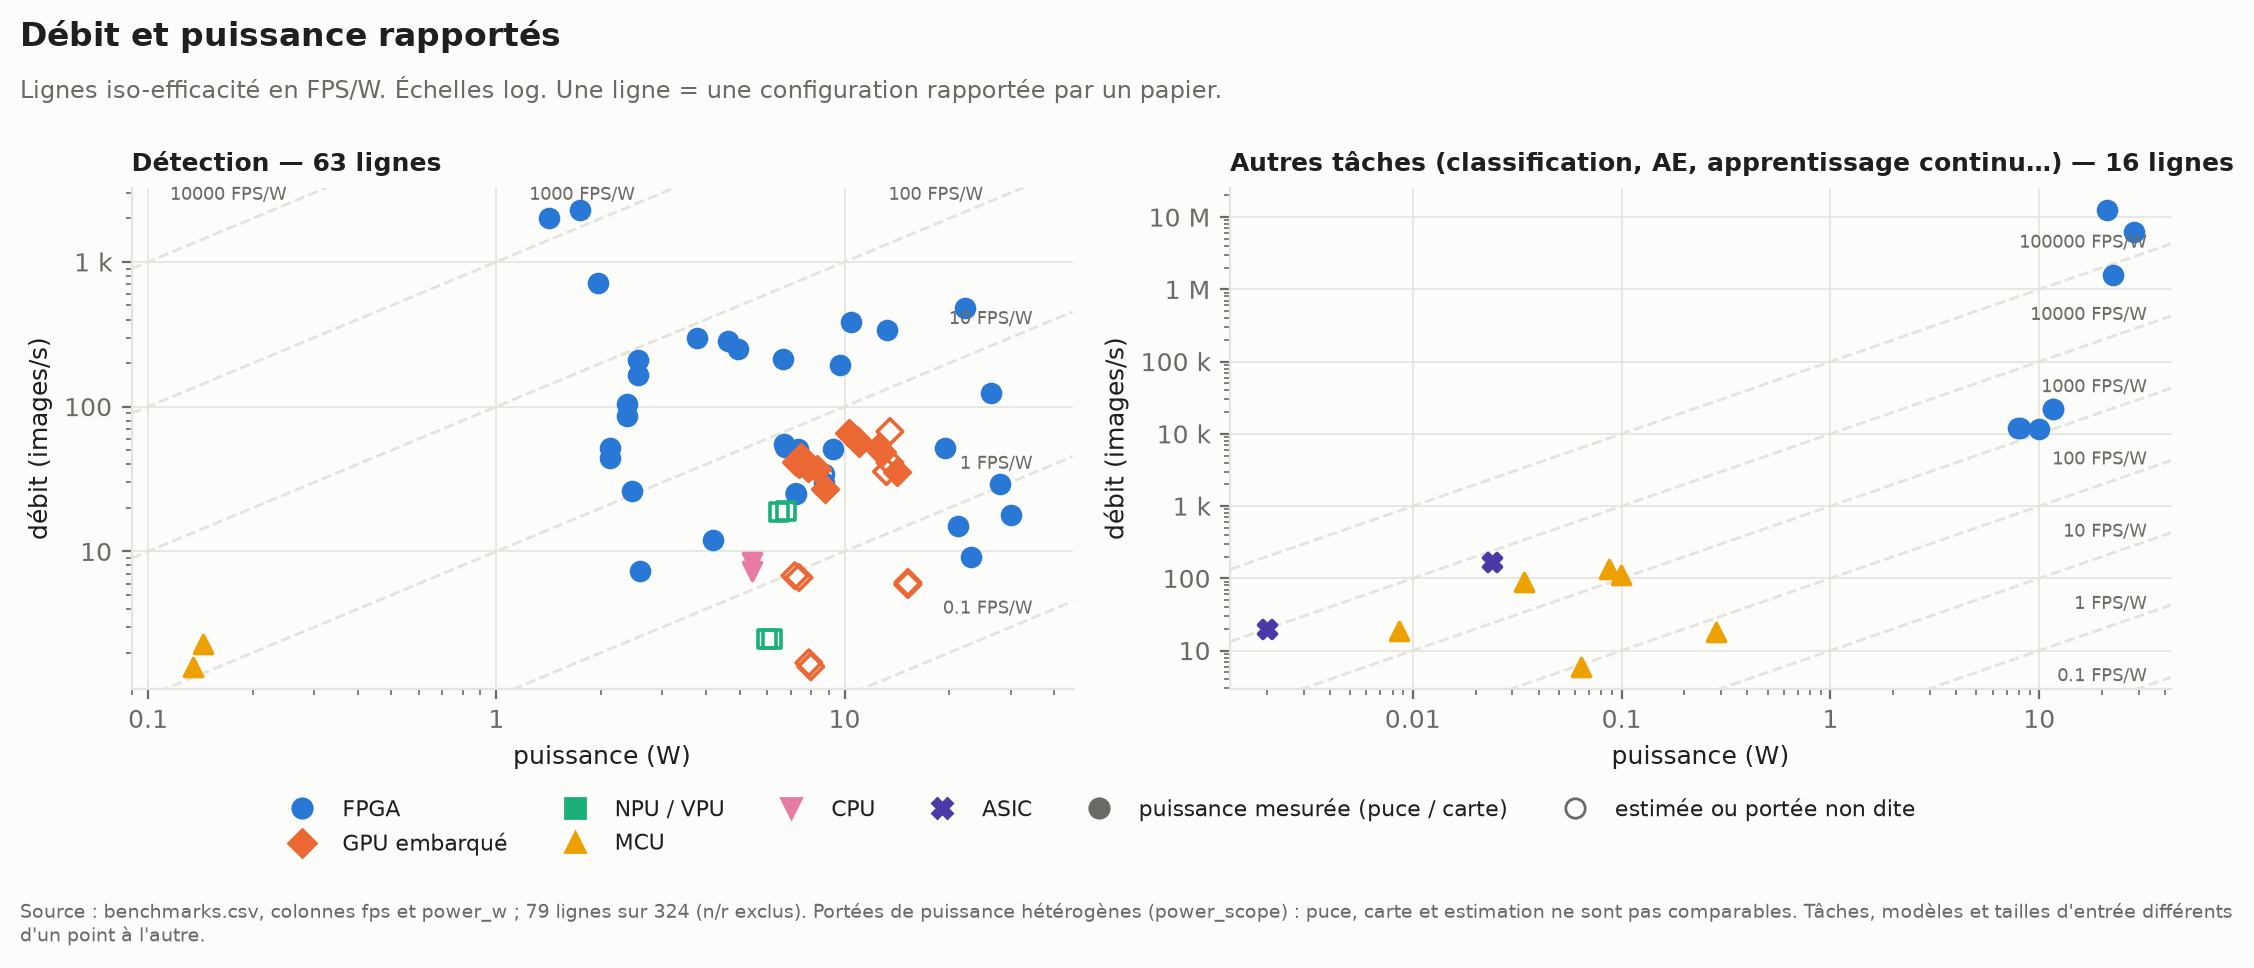
\includegraphics[width=\textwidth]{../../figures/bench_fps_power.png}
\caption{Débit et puissance rapportés, en échelles logarithmiques ; droites pointillées
d'iso-efficacité en FPS/W. Figure générée par \texttt{bin/pdb plot} à partir de
\texttt{benchmarks.csv} (28/09/2026).}
\label{fig:fps-power}
\end{figure}

Pour la détection (panneau de gauche), la figure montre trois groupes. Les deux points
\gl{MCU}{MCU} (SSD-MobileNetV2 sur GAP8) sont vers 0,14\,W et 2\,\gl{FPS}{FPS}. Les \gl{GPU}{GPU} embarqués (Jetson) se
regroupent entre 7 et 15\,W pour quelques dizaines d'images par seconde. Les \gl{FPGA}{FPGA}
s'étalent sur trois ordres de grandeur de débit, de 1,4 à 30\,W ; les points au-dessus de
1\,000\,FPS sont les réseaux minuscules du \gl{DAC-SDC}{DAC-SDC}, mesurés sans chargement d'images. Ce
que la figure ne permet pas : conclure qu'une famille est plus efficace qu'une autre.
Aucun couple de points ne partage à la fois le modèle, la résolution, la précision
numérique et la méthode de mesure \deduit.

\subsection{Les rares comparaisons à modèle égal}

\begin{table}[!htbp]
\centering\footnotesize
\caption{Comparaisons du corpus où un même réseau est mesuré sur plusieurs familles de
plateformes.}
\label{tab:meme-modele}
\begin{tabularx}{\textwidth}{@{}P{3.0cm}P{2.4cm}LP{3.2cm}@{}}
\toprule
Travail & Modèle & Résultat & Réserve \\
\midrule
SkyNet \citep{arxiv-1909.09709-skynet-hardware-efficient-method-object}\pp & SkyNet,
  DAC-SDC & TX2 : 67,3\,FPS, 13,5\,W ; Ultra96 : 25,1\,FPS, 7,3\,W \src{Tables~5--6} &
  portée non décrite ; \gl{lot}{lot de} 4 sur FPGA \\
SATAY \citep{2023-montgomerie-corcoran-satay-streaming-architecture-toolflow-accelerating} &
  YOLOv5n 640 & ZCU104 : 317\,mJ/image ; TX2 : 277\,mJ \src{Table~IV}\med & portée non
  décrite ; runtime du TX2 \nr \\
\citet{2025-elhence-fpga-accelerated-yolox-enhanced-attention} & LCAM-YOLOX & KV260 : 195\,FPS ;
  Jetson Nano : 65\,FPS ; STM32H7A3 : 15\,FPS \src{§V-D}\med & précision et puissance \nr{}
  hors FPGA ; chiffre MCU invraisemblable \\
TinyissimoYOLO \citep{arxiv-2306.00001-tinyissimoyolo-quantized-low-memory-footprint} & réseau
  88$\times$88 & MAX78000 : 5,5\,ms, 196\,µJ ; Apollo4b : 6,1\,mJ \src{§III}\med & MCU
  seulement \\
\citet{arxiv-2502.15737-performance-analysis-you-only-look} & YOLOv8n \gl{INT8}{INT8} & Orin NX :
  65,8\,FPS, 10,3\,W ; Orin Nano : 44,9\,FPS, 7,5\,W \src{Table~4} & Jetson seulement ;
  \gl{telemetrie}{télémétrie} ; jeu privé facile \\
\citet{arxiv-2409.16808-comprehensive-evaluation-deep-learning-object}\pp & YOLOv8n & Orin
  Nano : 16\,ms ; RPi~5 + Hailo-8 : 76\,ms ; \gl{mAP}{mAP} \gl{COCO}{COCO} 31--32 \src{§IV}\med & précision
  numérique \nr ; pas de FPGA \\
\citet{2022-feng-benchmark-analysis-yolo-performance-edge} & YOLOv3-tiny & Xavier NX :
  41,1\,FPS ; RPi + NCS2 : 18,8 ; Nano : 6,8 \src{Table~3} & pas de mAP ; sans TensorRT \\
\bottomrule
\end{tabularx}
\end{table}

Le tableau~\ref{tab:meme-modele} montre qu'aucun article ne mesure le même détecteur sur
les trois gammes (nano, FPGA, Jetson) avec la même portée de puissance. Les comparaisons
FPGA--Jetson existantes utilisent des Jetson de 2017 (TX2) ou des modèles minuscules ; la
seule qui ajoute un MCU (Elhence et al.) n'est pas crédible sur ce point. Les baselines
Jetson récentes (Orin, TensorRT INT8) existent dans le corpus
\citep{arxiv-2502.15737-performance-analysis-you-only-look}, mais sans FPGA en face.

\subsection{Ordres de grandeur par gamme}

Faute de comparaison directe, le corpus donne des ordres de grandeur, à ne lire que
comme tels :
\begin{itemize}
  \item \textbf{nano} : de 4 à 41\,\gl{MAC}{MMAC} par image pour la navigation, 534\,MMAC pour le
    seul détecteur déployé (SSD-MbV2, 1,6\,FPS) ; de 34 à 284\,mW ; 0,4\,mJ par image pour
    la pose humaine \citep[§V-B]{arxiv-2103.10873-fully-onboard-ai-powered-human}\pp ;
  \item \textbf{FPGA} : de 2,5\,W (Zynq-7020, carte) à 10\,W (KV260, carte) et 30\,W (ZCU104,
    à la prise), pour des \gl{YOLO}{YOLO} réduits à quelques centaines de FPS d'accélérateur, et
    quelques dizaines de \gl{bout}{bout en bout} ;
  \item \textbf{Jetson} : de 7 à 15\,W de télémétrie pour YOLOv8n et YOLOv8s en INT8
    (45 à 66\,FPS), 40\,ms pour les réseaux de vol agile sur TX2, de 23 à 35\,FPS pour les
    trackers et GLAD sur Xavier.
\end{itemize}
L'écart entre gammes est de l'ordre de trois ordres de grandeur en puissance, mais la
tâche change aussi : navigation en 200$\times$200 en niveaux de gris d'un côté, détection
en 640$\times$640 de l'autre \deduit.

\subsection{Couverture du corpus}

La figure~\ref{fig:gaps-map} croise la famille de plateforme des mesures et l'axe des
articles. Elle confirme les déséquilibres décrits dans ce document : la détection drone
est surtout mesurée sur GPU de bureau (17 articles), le contre-drone aussi (9 articles),
aucune mesure FPGA ne concerne un nano-drone et aucune mesure du corpus ne porte sur la
fiabilité. Un zéro signifie \enquote{absent de la base}, pas \enquote{absent de la
littérature}.

\begin{figure}[!htbp]
\centering
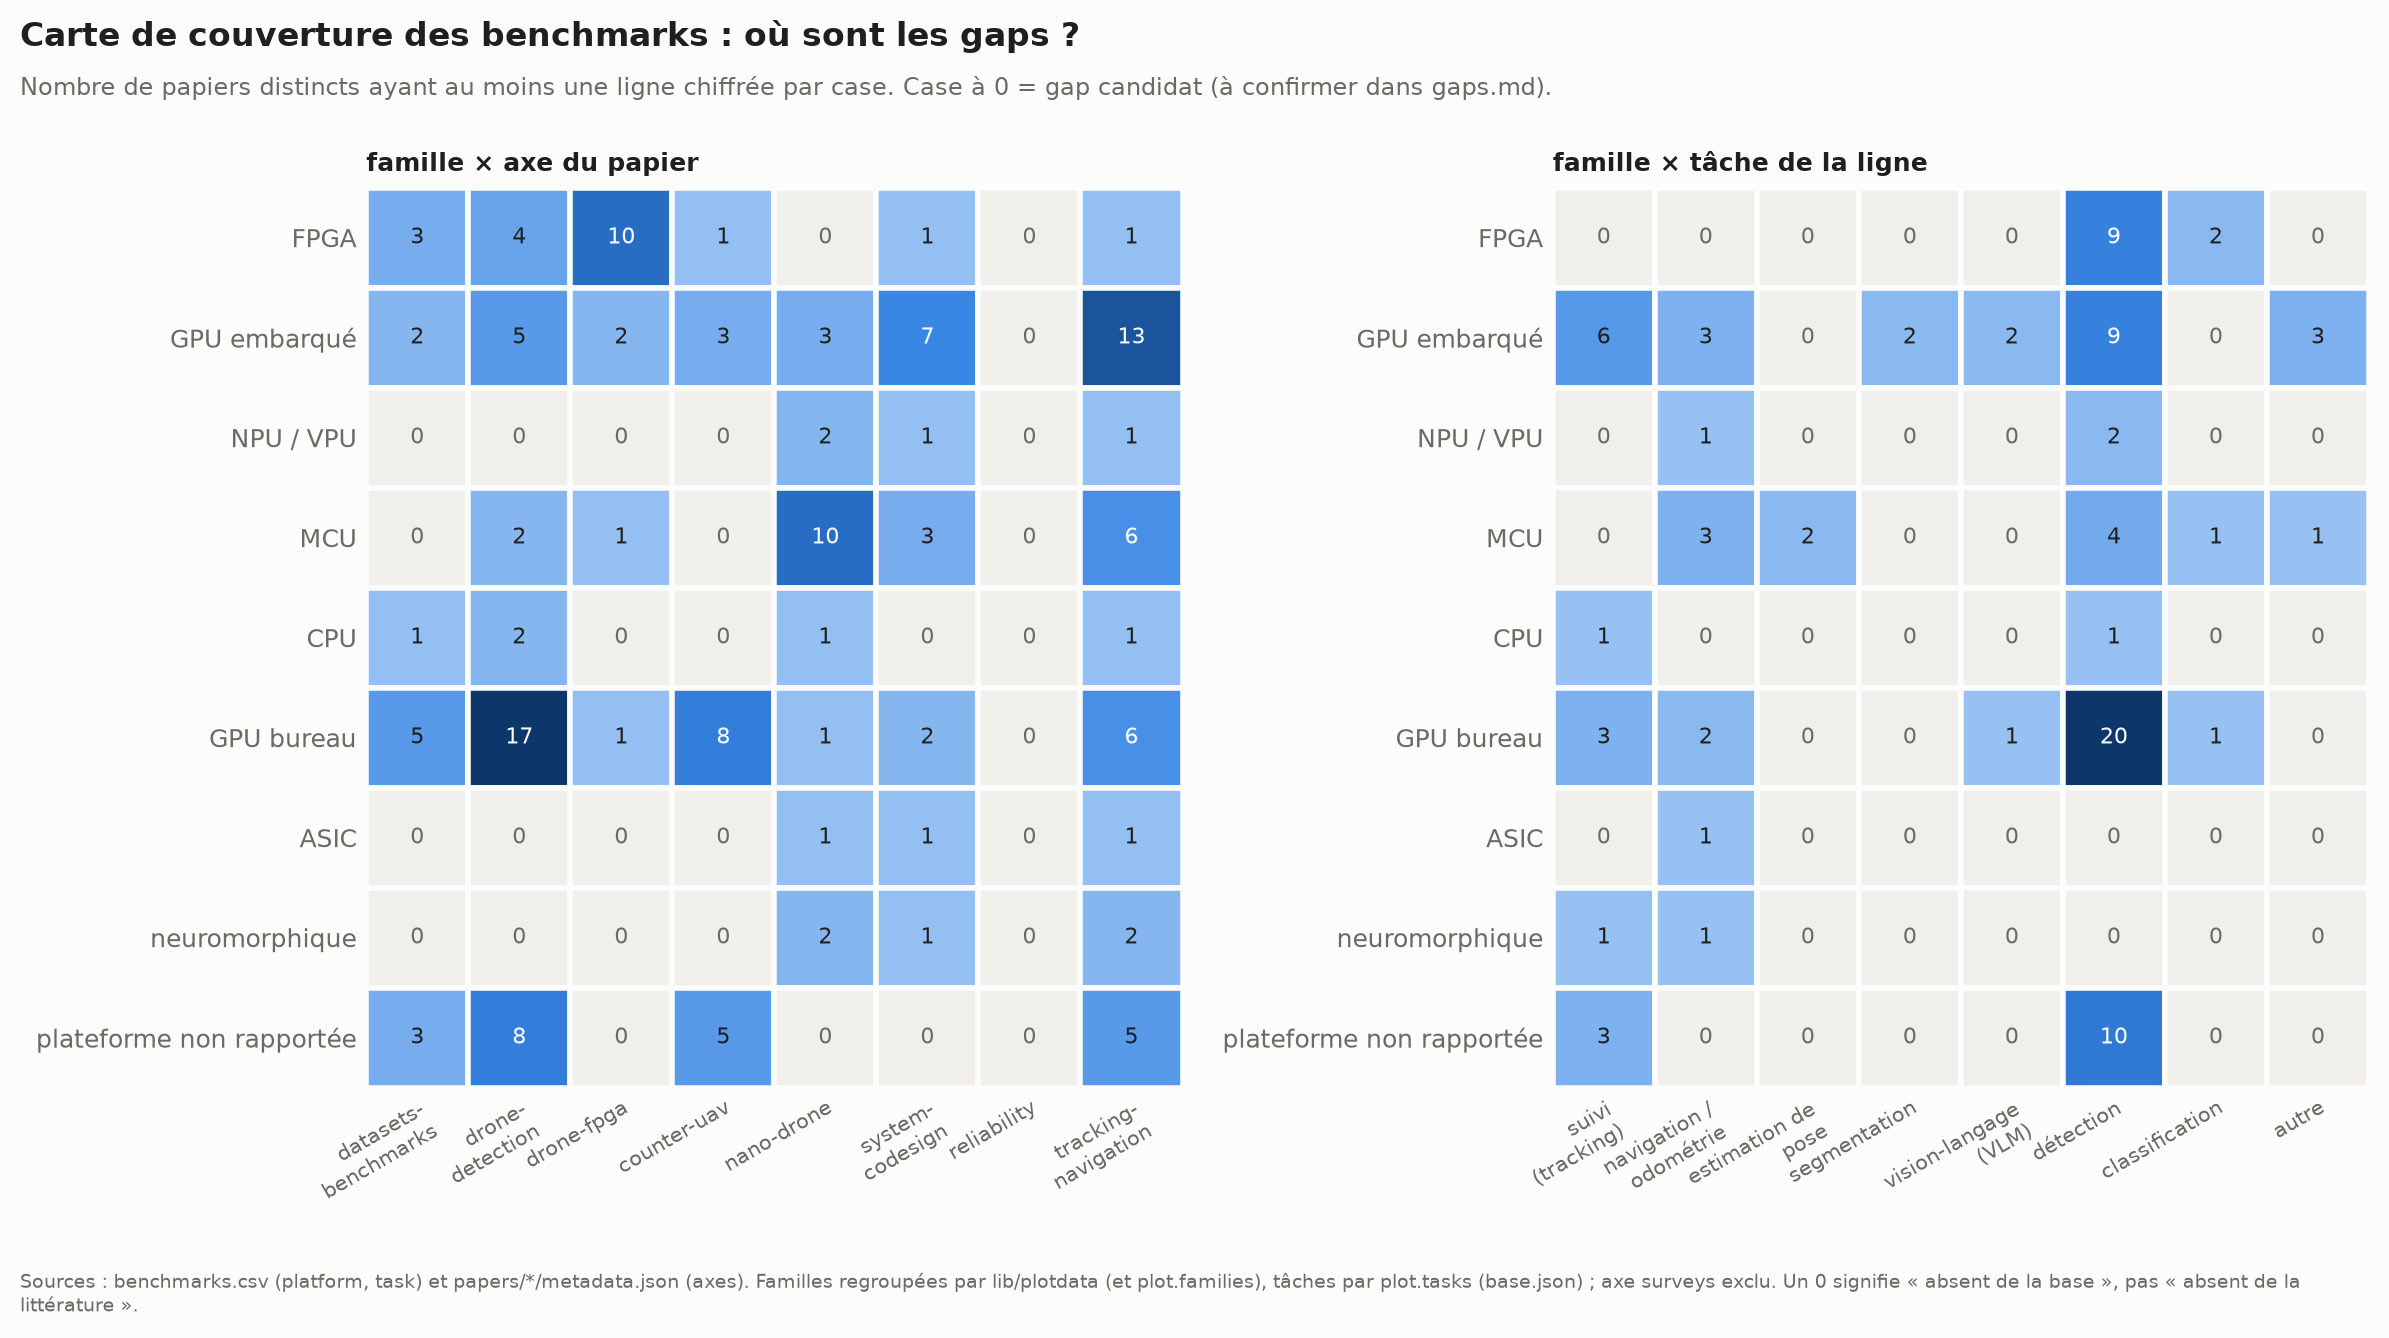
\includegraphics[width=\textwidth]{../../figures/corpus_gaps.png}
\caption{Nombre d'articles ayant au moins une ligne chiffrée, par famille de plateforme et
par axe (gauche) ou tâche (droite). Figure générée par \texttt{bin/pdb plot} (28/09/2026).}
\label{fig:gaps-map}
\end{figure}

% Gaps (repris de gaps.md, 2e passe du 28/09/2026) et questions de thèse
\section{Zones non couvertes et pistes de recherche}
\label{sec:gaps}

Les gaps ci-dessous viennent de \texttt{gaps.md} (2\textsuperscript{e} passe, 28/09/2026,
73 fiches et 324 lignes). Un gap \emph{étayé} est constaté dans plusieurs fiches (mesure
absente, limite reconnue par les auteurs) ; cela ne prouve pas qu'il est absent de la
littérature. Un gap à l'état d'\emph{hypothèse} ne repose que sur l'absence de papiers
dans la base.

\begin{table}[!htbp]
\centering\footnotesize
\caption{Gaps du corpus drone : statut et piste principale.}
\label{tab:gaps}
\begin{tabularx}{\textwidth}{@{}P{4.3cm}P{1.8cm}L@{}}
\toprule
Gap & Statut & Piste \\
\midrule
Décalage algorithme / matériel : \gl{YOLO}{YOLO} drone (P2, \gl{attention}{attention}) jamais portés sur \gl{FPGA}{FPGA} & étayé &
  YOLOv8n-P2 ou Drone-YOLO nano en \gl{INT8}{INT8} sur KV260 (Vitis~AI), contre \gl{FINN}{FINN} ou hls4ml ; \gl{mAP}{mAP}
  VisDrone avant et après \\
Quantification et petits objets : 0 ligne avec \gl{APS}{AP$_S$} sur 324 & étayé & balayage \gl{PTQ}{PTQ} / \gl{QAT}{QAT}
  (\gl{FP32}{FP32}, INT8, INT4) d'un YOLO drone sur VisDrone, \gl{AP}{AP}$_S$ mesurée sur la carte \\
Tête P2 et haute résolution : coût mémoire on-chip non mesuré & étayé (coût) ; hypothèse
  (absence FPGA) & tailles d'activation par couche de YOLOv8n et YOLOv8n-P2 face au budget
  \gl{BRAM}{BRAM} d'un ZU3EG ou d'une KV260 \\
Paramètres et \gl{FLOPs}{FLOPs} $\neq$ latence sur cible & étayé & trois variantes légères d'un même
  YOLO profilées sur KV260 et Orin, à précision égale \\
Post-traitement sur le \gl{PS}{PS} : goulot de \gl{bout}{bout en bout} & étayé & \gl{NMS}{NMS} matériel ou tête sans NMS ;
  latence caméra $\rightarrow$ sortie instrumentée \\
Calcul adaptatif ou épars jamais évalué à bord & étayé & SAHI à tuiles fixes contre saut de
  tuiles vides sur KV260, latence au pire cas \\
Métriques non comparables ; benchmarks sans métrique d'efficacité & étayé & protocole
  commun : métrique, résolution, \gl{portee}{portée} de la puissance \\
Métrique système absente des papiers YOLO/FPGA & étayé & designs FPGA publiés placés sur le
  \gl{roofline}{modèle F-1} avec masse de carte mesurée \\
Fiabilité des accélérateurs de détection sur drone & étayé (corpus mince) & injection de
  fautes sur un détecteur FPGA avec métrique de mission \\
Pas de comparaison entre \gl{gamme}{gammes de puissance} & étayé & même réseau, même entrée, même
  portée de puissance sur GAP8, FPGA et Jetson \\
Détection et navigation sur le même budget & étayé & partage d'un \gl{SoC}{SoC} par reconfiguration
  partielle, interférence mesurée \\
Suivi embarqué sans puissance ni FPGA & étayé & HiFT ou SiamAPN++ sur FPGA, énergie par
  image \\
Contre-drone évalué sur \gl{GPU}{GPU} de bureau & étayé & YOLOv8n sur Det-Fly, INT8 sur KV260 contre
  Orin, puissance à la carte \\
Détecteur \gl{airair}{air $\rightarrow$ air} embarqué sur intercepteur & étayé & détecteur sur SoC avec
  AP, \gl{FPS}{FPS}, W et latence de bout en bout ; Det-Fly et ARD-MAV \\
Air $\rightarrow$ air : coût du mouvement multi-images & étayé (coût) ; hypothèse (FPGA) &
  profil par étage de GL-YOMO ou GLAD ; tampon on-chip de 8 images \\
Fusion visible + thermique à bord & hypothèse & recherche ciblée (\texttt{/paper-discover}) \\
Apprentissage continu à bord du drone & hypothèse & base \texttt{fpga} ; recherche ciblée \\
Code et bitstreams rarement publiés & étayé (relevé approximatif) & distinguer code
  d'entraînement et design matériel \\
\bottomrule
\end{tabularx}
\end{table}

\subsection{Trois gaps structurants}

\paragraph{Le décalage algorithme / matériel.} C'est l'hypothèse de départ de la base, et
le corpus l'étaye. Les détecteurs qui font l'état de l'art sur VisDrone ajoutent une tête
P2 et de l'attention (section~\ref{sec:detection}). Les implantations FPGA restent sur des
YOLO anciens et, pour tenir, retirent la branche multi-échelle
\citep{2025-cali-optimized-implementation-yolov3-tiny-real} ou remplacent l'attention
\citep{arxiv-2607.13106-no-attention-no-problem-dpu}\pp. La seule mesure embarquée d'une
\gl{teteP2}{tête P2} (Jetson TX2) montre un facteur 3 à 4 en latence
\citep[Table~6]{2023-zhang-drone-yolo-efficient-neural-network}. Deux familles
d'alternatives à P2 existent, jamais évaluées sur FPGA : transférer l'information de P2
vers P3 (TPH-YOLOv5++), ou recadrer à pleine résolution autour des régions utiles (SAHI,
UFPMP-Det, GLAD).

\paragraph{La précision sur petits objets après quantification.} Aucune des 324 lignes ne
rapporte d'AP$_S$. Les pertes de \gl{quantif}{quantification} connues sont globales et souvent fortes
(6 à 30 points de mAP selon le modèle et le jeu). On ne sait donc pas si la
quantification, indispensable sur FPGA et \gl{MCU}{MCU}, détruit précisément ce que les YOLO drone
cherchent à gagner.

\paragraph{La métrique de mission.} Le lien entre latence, masse et \gl{vitesse}{vitesse sûre} est
modélisé \citep{arxiv-2204.10898-roofline-model-uavs-bottleneck-analysis}\pp{} et mesuré
pour des nano-drones, jamais pour un détecteur sur FPGA. Le modèle lui-même ignore la
qualité de perception, et la gamme nano montre qu'un réseau plus rapide peut moins bien
servir la mission \citep[Table~IV]{arxiv-2103.10873-fully-onboard-ai-powered-human}\pp.

\subsection{Questions de thèse candidates}

Les trois questions ci-dessous sont des déductions à partir des gaps, pas des
conclusions du corpus.
\begin{enumerate}
  \item \textbf{Détecteur air $\rightarrow$ air sur SoC embarquable.} Peut-on détecter un
    drone de quelques pixels à bord d'un intercepteur, sur KV260 ou Zynq UltraScale+, avec
    une AP, une latence de bout en bout et une puissance à la carte mesurées, et comment
    se compare-t-on à une Jetson Orin à protocole égal ? Données : Det-Fly, ARD-MAV,
    NPS-Drones. Point de départ : l'architecture globale/locale de GLAD, dont la partie
    non neuronale est à accélérer.
  \item \textbf{Petits objets et précision numérique.} Quelle est la perte d'AP$_S$ d'un
    YOLO drone (avec et sans tête P2) quand on passe de FP32 à INT8 puis INT4, en PTQ et en
    QAT, mesurée sur la carte ? Quelle alternative à P2 (recadrage, transfert vers P3) tient
    dans la mémoire on-chip d'une petite FPGA à précision égale ?
  \item \textbf{Du FPS à la vitesse sûre.} Comment traduire le débit, la puissance et la
    masse d'un accélérateur de détection en vitesse de vol sûre et en autonomie, en
    intégrant la qualité de détection au modèle F-1 ? À quelle gamme de puissance
    (nano, FPGA, Jetson) correspond l'optimum pour un drone donné ?
\end{enumerate}
Laboratoires français à approcher : \texttt{labs.md} ne recense encore que le LIRMM (test
et fiabilité), sans papier du corpus à l'appui ; la liste reste à construire.


\section{Conclusion}

La vision embarquée sur drone dispose de jeux de données de référence (VisDrone, UAVDT,
\glslink{dac-sdc}{DAC-SDC}, Det-Fly), d'une littérature abondante de détecteurs pour petits objets et de
démonstrations convaincantes dans chaque \glslink{gamme}{gamme de puissance} : \glslink{ssd-mobilenetv2}{SSD-MobileNetV2} sur \glslink{gap8}{GAP8} à
134\,\glslink{u-mw}{mW}, \glslink{yolox}{YOLOX} sur \glslink{kv260}{KV260} à 10\,\glslink{u-w}{W}, perception et contrôle de course sur \glslink{tx2}{Jetson TX2},
suivi agile et détection air $\rightarrow$ air en vol sur \glslink{orin-nx}{Jetson Orin NX}. Le
corpus montre pourtant que ces trois littératures se croisent peu :
\begin{itemize}
  \item les détecteurs les plus précis sur VisDrone sont mesurés sur \gl{GPU}{GPU} de bureau, et le
    seul portage embarqué d'une \glslink{p2head}{tête P2} (\glslink{drone-yolo}{Drone-YOLO} sur \glslink{tx2}{TX2}) coûte un facteur 3 à 4 en
    latence ;
  \item les designs \gl{FPGA}{FPGA} optimisent le débit sur des réseaux minuscules (\glslink{dac-sdc}{DAC-SDC}) ou
    simplifiés, avec des précisions non comparables et sans \glslink{aps}{AP$_S$} ;
  \item le co-design calcul--vol est modélisé, rarement mesuré, et jamais pour un FPGA ;
  \item le contre-drone \gl{airair}{air $\rightarrow$ air} a des jeux publics (Det-Fly, NPS-Drones,
    ARD-MAV) mais deux chiffres embarqués seulement (\glslink{glad}{GLAD}, SCOUT), tous deux sur \glslink{jetson}{Jetson} et sans
    puissance ; seul SCOUT ferme la boucle en vol, en salle et sans taux d'interception ;
  \item la navigation et les modèles vision-langage embarqués sur \glslink{orin}{Orin} (profondeur,
    segmentation, appariement d'images) ont un goulot de perception dense jamais mesuré en
    puissance ni porté sur FPGA ; le \glslink{gap9}{GAP9}, nouvelle génération nano, n'a encore ni puissance
    mesurée ni détecteur dans le corpus.
\end{itemize}
Ces manques dessinent un sujet de thèse cohérent : porter un détecteur de petits objets
récent sur un \gl{SoC}{SoC} embarquable, mesurer honnêtement sa précision par taille d'objet et sa
puissance à la carte, et traduire le résultat en métrique de mission.

\paragraph{Pistes concrètes.}
\begin{enumerate}
  \item \textbf{Papier à lire en priorité} : les deux références de
    \citet{2025-hozhabr-survey-real-time-object-detection} sur le post-traitement matériel
    (\glslink{nms}{NMS} pipeliné d'Anupreetham et al., système tout-FPGA de D.~Zhang et al.), absentes de
    la base : elles répondent au goulot \gl{PS}{PS} observé dans quatre papiers.
  \item \textbf{Expérience à reproduire} : \glslink{yolov8n}{YOLOv8n} entraîné sur Det-Fly
    \citep{2021-zheng-air-air-visual-detection-micro}, en \gl{INT8}{INT8} sur \glslink{kv260}{KV260} (Vitis~AI) et sur
    \glslink{orin}{Jetson Orin}, avec \glslink{ap}{AP} et \glslink{aps}{AP$_S$} mesurées sur la carte, latence de \gl{bout}{bout en bout} et
    puissance à la carte des deux côtés.
  \item \textbf{Gap à creuser} : placer les designs de
    \citet{2025-cali-optimized-implementation-yolov3-tiny-real} et
    \citet{2025-elhence-fpga-accelerated-yolox-enhanced-attention} sur le \gl{roofline}{modèle F-1} de
    \citet{arxiv-2204.10898-roofline-model-uavs-bottleneck-analysis}, pour obtenir la
    première métrique de \glslink{vsure}{vitesse sûre} d'un détecteur FPGA.
\end{enumerate}

\bibliographystyle{plainnat}
\bibliography{refs}

\appendix
% Généré par glossify.py : glossaire des acronymes et lexique (cibles des liens \gl)
\section{Glossaire des acronymes}
\label{sec:acronymes}

{\small
\begin{longtable}{@{}>{\raggedright\arraybackslash}p{2.2cm}>{\raggedright\arraybackslash}p{\dimexpr\linewidth-2.2cm-2\tabcolsep\relax}@{}}
\toprule
Acronyme & Signification \\
\midrule
\endhead
\leavevmode\hypertarget{gl:AP}{AP} & \emph{Average Precision}, précision moyenne d'un détecteur (aire sous la courbe précision--rappel) ; \gl{mAP}{mAP} si moyennée sur les classes \\
\leavevmode\hypertarget{gl:ASIC}{ASIC} & \emph{Application-Specific Integrated Circuit}, circuit intégré conçu pour une seule fonction \\
\leavevmode\hypertarget{gl:AUC}{AUC} & \emph{Area Under the Curve}, aire sous la courbe de succès en suivi d'objet \\
\leavevmode\hypertarget{gl:BRAM}{BRAM} & \emph{Block RAM}, mémoire embarquée d'un FPGA ; avec l'URAM, elle borne ce qui tient sur la puce \\
\leavevmode\hypertarget{gl:CNN}{CNN} & \emph{Convolutional Neural Network}, réseau de neurones convolutif \\
\leavevmode\hypertarget{gl:COCO}{COCO} & \emph{Common Objects in Context}, jeu de détection généraliste (80 classes) et protocole d'AP moyenné sur les seuils d'IoU 0,5 à 0,95 \\
\leavevmode\hypertarget{gl:CPU}{CPU} & \emph{Central Processing Unit}, processeur généraliste \\
\leavevmode\hypertarget{gl:DAC-SDC}{DAC-SDC} & \emph{Design Automation Conference -- System Design Contest}, concours de détection basse consommation sur images de drone, plateformes imposées (PYNQ-Z1, Ultra96, Jetson TX2) \\
\leavevmode\hypertarget{gl:DMA}{DMA} & \emph{Direct Memory Access}, transfert mémoire sans intervention du processeur \\
\leavevmode\hypertarget{gl:DPU}{DPU} & \emph{Deep-learning Processing Unit}, accélérateur CNN générique de Vitis~AI (AMD-Xilinx), programmé par instructions, en INT8 \\
\leavevmode\hypertarget{gl:DSP}{DSP} & \emph{Digital Signal Processing (bloc)}, multiplieur-accumulateur câblé d'un FPGA \\
\leavevmode\hypertarget{gl:DVS}{DVS} & \emph{Dynamic Vision Sensor}, caméra événementielle : chaque pixel émet un événement quand sa luminosité change \\
\leavevmode\hypertarget{gl:FINN}{FINN} & \emph{FINN (AMD-Xilinx)}, toolflow dataflow open source pour réseaux quantifiés sur FPGA \\
\leavevmode\hypertarget{gl:FLOPs}{FLOPs} & \emph{Floating-Point Operations}, nombre d'opérations d'une inférence (GFLOPs : milliards) ; mesure de coût théorique, pas de latence \\
\leavevmode\hypertarget{gl:FP32}{FP32} & \emph{Floating Point 32 bits}, flottant simple précision ; FP16 : demi-précision \\
\leavevmode\hypertarget{gl:FPGA}{FPGA} & \emph{Field-Programmable Gate Array}, circuit logique reprogrammable ; en SoC (Zynq, Kria), associé à des cœurs ARM \\
\leavevmode\hypertarget{gl:FPS}{FPS} & \emph{Frames Per Second}, images par seconde (débit) \\
\leavevmode\hypertarget{gl:GOPS}{GOPS} & \emph{Giga Operations Per Second}, milliards d'opérations par seconde \\
\leavevmode\hypertarget{gl:GPU}{GPU} & \emph{Graphics Processing Unit}, processeur graphique ; « GPU de bureau » (RTX, Titan, Tesla) par opposition au GPU embarqué des Jetson \\
\leavevmode\hypertarget{gl:AI}{IA} & intelligence artificielle \\
\leavevmode\hypertarget{gl:INT8}{INT8} & \emph{entiers sur 8 bits}, précision numérique après quantification ; INT4 : 4 bits \\
\leavevmode\hypertarget{gl:IoU}{IoU} & \emph{Intersection over Union}, recouvrement entre boîte prédite et boîte réelle ; au DAC-SDC, IoU moyen d'un objet unique, qui n'est pas une mAP \\
\leavevmode\hypertarget{gl:MAC}{MAC} & \emph{Multiply-Accumulate}, multiplication-accumulation ; MMAC, GMAC : millions, milliards \\
\leavevmode\hypertarget{gl:mAP}{mAP} & \emph{mean Average Precision}, AP moyennée sur les classes ; mAP50 ou AP50 : au seuil d'IoU 0,5 ; mAP50-95 : protocole COCO \\
\leavevmode\hypertarget{gl:MCU}{MCU} & \emph{Microcontroller Unit}, microcontrôleur (Cortex-M, GAP8, MAX78000) \\
\leavevmode\hypertarget{gl:mSA}{mSA} & \emph{mean State Accuracy}, métrique des jeux Anti-UAV : IoU quand la cible est visible, prédiction d'absence sinon \\
\leavevmode\hypertarget{gl:NMS}{NMS} & \emph{Non-Maximum Suppression}, suppression des boîtes de détection en double, en post-traitement \\
\leavevmode\hypertarget{gl:NPU}{NPU} & \emph{Neural Processing Unit}, accélérateur de réseaux de neurones (Hailo-8, Edge TPU, VPU Myriad) \\
\leavevmode\hypertarget{gl:PID}{PID} & \emph{Proportionnel-Intégral-Dérivé}, régulateur classique du contrôle de vol \\
\leavevmode\hypertarget{gl:PS}{PS} & \emph{Processing System}, partie processeur (cœurs ARM) d'un SoC FPGA ; PL : logique programmable \\
\leavevmode\hypertarget{gl:PTQ}{PTQ} & \emph{Post-Training Quantization}, quantification après entraînement, avec un jeu de calibration \\
\leavevmode\hypertarget{gl:QAT}{QAT} & \emph{Quantization-Aware Training}, entraînement qui simule la quantification, en général moins coûteux en précision que la PTQ \\
\leavevmode\hypertarget{gl:SEU}{SEU} & \emph{Single Event Upset}, inversion d'un bit par une particule (radiations) ; la mémoire de configuration d'un FPGA y est sensible \\
\leavevmode\hypertarget{gl:SNN}{SNN} & \emph{Spiking Neural Network}, réseau de neurones impulsionnels, exécuté sur puce neuromorphique (Loihi) \\
\leavevmode\hypertarget{gl:SoC}{SoC} & \emph{System on Chip}, puce intégrant processeurs et accélérateurs (SoC FPGA : Zynq, Kria) \\
\leavevmode\hypertarget{gl:SRAM}{SRAM} & \emph{Static RAM}, mémoire statique ; dans un FPGA, elle stocke aussi la configuration \\
\leavevmode\hypertarget{gl:SSD}{SSD} & \emph{Single Shot MultiBox Detector}, détecteur à un étage, souvent avec backbone MobileNet \\
\leavevmode\hypertarget{gl:TDP}{TDP} & \emph{Thermal Design Power}, puissance thermique nominale d'une puce, pas sa consommation mesurée \\
\leavevmode\hypertarget{gl:UWB}{UWB} & \emph{Ultra-Wideband}, radio à bande ultra-large, utilisée pour la télémétrie de distance \\
\leavevmode\hypertarget{gl:VOC}{VOC} & \emph{PASCAL Visual Object Classes}, jeu de détection généraliste (20 classes) \\
\leavevmode\hypertarget{gl:YOLO}{YOLO} & \emph{You Only Look Once}, famille de détecteurs d'objets à un étage (v3 à v26) \\
\bottomrule
\end{longtable}}

\clearpage
\section{Lexique}
\label{sec:lexique}

{\small
\begin{longtable}{@{}>{\raggedright\arraybackslash}p{4.2cm}>{\raggedright\arraybackslash}p{\dimexpr\linewidth-4.2cm-2\tabcolsep\relax}@{}}
\toprule
Terme & Sens dans ce document \\
\midrule
\endhead
\leavevmode\hypertarget{gl:airair}{air $\rightarrow$ air} & contre-drone où le détecteur est à bord d'un drone (intercepteur) ; seul cas qui relève de l'IA embarquée \\
\leavevmode\hypertarget{gl:APS}{AP$_S$} & AP sur les petits objets (moins de 32$\times$32 pixels, protocole COCO) \\
\leavevmode\hypertarget{gl:attention}{attention} & mécanisme qui pondère les caractéristiques selon leur pertinence (canal, espace, ou attention matricielle des Transformer) \\
\leavevmode\hypertarget{gl:backbone}{backbone} & partie du réseau qui extrait les caractéristiques, avant le neck et les têtes \\
\leavevmode\hypertarget{gl:boucle}{boucle fermée} & la perception pilote réellement le drone pendant l'essai, par opposition à une évaluation sur données enregistrées \\
\leavevmode\hypertarget{gl:bout}{bout en bout (latence, débit)} & de l'acquisition de l'image à la sortie des boîtes, pré- et post-traitement compris \\
\leavevmode\hypertarget{gl:dataflow}{dataflow, streaming} & architecture d'accélérateur où chaque couche a son propre bloc matériel, les données circulant en flux entre blocs \\
\leavevmode\hypertarget{gl:deduit}{déduit} & inférence de la fiche ou de ce document, par opposition à ce que disent les auteurs \\
\leavevmode\hypertarget{gl:depthwise}{depthwise, GhostConv} & convolutions allégées (par canal, ou générant une partie des cartes par opérations bon marché) ; peu de FLOPs mais souvent mal servies par les accélérateurs \\
\leavevmode\hypertarget{gl:dsppacking}{DSP packing} & calcul de plusieurs multiplications à faible précision dans un même bloc DSP \\
\leavevmode\hypertarget{gl:egomotion}{ego-motion} & mouvement propre de la caméra embarquée, à compenser avant d'exploiter le mouvement de la cible \\
\leavevmode\hypertarget{gl:elagage}{élagage (pruning)} & suppression de canaux, de couches ou de poids ; seul l'élagage structuré accélère sur matériel \\
\leavevmode\hypertarget{gl:flot}{flot optique} & champ de déplacement apparent des pixels entre deux images \\
\leavevmode\hypertarget{gl:gamme}{gamme de puissance} & nano (mW), FPGA (W), Jetson (autour de 10\,W) ; tout résultat y est situé \\
\leavevmode\hypertarget{gl:hil}{hardware-in-the-loop} & simulation du drone et de son environnement avec le calculateur réel dans la boucle \\
\leavevmode\hypertarget{gl:lot}{lot (batch)} & nombre d'images traitées ensemble ; un débit en lot n'est pas une latence par image \\
\leavevmode\hypertarget{gl:nr}{\texttt{n/r}} & valeur non rapportée par les auteurs ; jamais estimée \\
\leavevmode\hypertarget{gl:pixthr}{pixel throughput} & débit normalisé par la résolution : FPS $\times$ pixels par image \\
\leavevmode\hypertarget{gl:genou}{point de genou} & dans le modèle F-1, débit de décision au-delà duquel accélérer le calcul n'augmente plus la vitesse sûre \\
\leavevmode\hypertarget{gl:portee}{portée de la puissance} & ce que couvre une puissance : carte entière (board), puce (chip), estimée (outil) ou non décrite \\
\leavevmode\hypertarget{gl:preprint}{preprint (\textsuperscript{\textsc{pp}})} & article déposé sur arXiv, non relu par les pairs dans la version ingérée \\
\leavevmode\hypertarget{gl:quantif}{quantification} & passage des poids et activations à une précision réduite (INT8, INT4, W4/A4) \\
\leavevmode\hypertarget{gl:roofline}{roofline, modèle F-1} & modèle de performance borné par le calcul et la mémoire ; F-1 : sa version pour drone, qui borne la vitesse sûre \\
\leavevmode\hypertarget{gl:solair}{sol $\rightarrow$ air} & contre-drone où le capteur est fixe au sol \\
\leavevmode\hypertarget{gl:sortie}{sortie anticipée (early-exit)} & arrêt de l'inférence à une couche intermédiaire quand une branche légère juge le résultat suffisant \\
\leavevmode\hypertarget{gl:soustraction}{soustraction de fond} & détection de ce qui bouge par différence avec un modèle du fond ; suppose une caméra fixe \\
\leavevmode\hypertarget{gl:spacedepth}{space-to-depth} & réorganisation d'une carte spatiale en canaux, qui garde le détail sans augmenter la résolution traitée \\
\leavevmode\hypertarget{gl:telemetrie}{télémétrie} & mesure de puissance par les capteurs de la carte (tegrastats, PMIC) ; portée puce ou module \\
\leavevmode\hypertarget{gl:testdev}{test-dev, validation} & splits d'évaluation de VisDrone ; les chiffres de l'un ne se comparent pas à ceux de l'autre \\
\leavevmode\hypertarget{gl:toolflow}{toolflow} & chaîne automatique qui transforme un réseau entraîné en accélérateur (FINN, SATAY, Vitis~AI) \\
\leavevmode\hypertarget{gl:siamois}{tracker siamois} & tracker qui compare un gabarit de la cible à une zone de recherche avec un même réseau \\
\leavevmode\hypertarget{gl:transformer}{Transformer} & bloc à attention multi-têtes, issu du traitement du langage \\
\leavevmode\hypertarget{gl:tuilage}{tuilage} & découpage d'une image haute résolution en tuiles inférées séparément \\
\leavevmode\hypertarget{gl:teteP2}{tête P2 (et P5)} & tête de détection sur la carte de stride 4 (160$\times$160 pour une entrée de 640), pour les petits objets ; P5 : stride 32, grands objets \\
\leavevmode\hypertarget{gl:vitesse}{vitesse sûre} & vitesse maximale à laquelle le drone peut encore s'arrêter avant un obstacle détecté \\
\leavevmode\hypertarget{gl:wa}{W$x$/A$y$} & précision numérique : poids sur $x$ bits, activations sur $y$ bits \\
\bottomrule
\end{longtable}}


\clearpage
\section*{Glossaires}
\addcontentsline{toc}{section}{Glossaires}
Chaque entrée renvoie aux sections où le terme apparaît ; dans le texte, chaque apparition
est un lien vers son entrée. Une valeur suivie de \constr{} vient de la documentation du
constructeur, \horscorpus{} de connaissances générales : ni l'une ni l'autre n'est tirée du
corpus. Les acronymes et le vocabulaire propre à ce document sont dans les deux annexes
précédentes.
\printglossary[type=plateformes]
\printglossary[type=modeles]
\printglossary[type=metriques]

\end{document}
